\documentclass[12pt, english]{book}
\usepackage{142crstyle}

% Created: Enze Chen and Aaron Lindenberg, May 2017
% Last edited: Enze Chen, September 2025

% This is the main .tex file that compiles all of the separate chapters together. 
% It uses the custom mystyle.sty style package and only has title page information below. 
% Changes to the chapters and appendices should be made in the respective file; changes here should be for organizational purposes only.

% Title and author information
\title{{\LARGE \textbf{MATSCI 142}} \\ Quantum Mechanics of Nanoscale Materials \vspace{10ex}}
\author{\vspace{1ex} Aaron M. Lindenberg \\ 
	    \vspace{1ex} Department of Materials Science and Engineering \\
	    \vspace{1ex} Stanford University \\ 
	    \vspace{1ex} Autumn 2025 (2$^{\text{nd}}$ ed.)
	    % \vspace{1ex} Spring 2018 (1$^{\text{st}}$ ed.) 
}
\date{}

\begin{document}
	
\frontmatter % Roman numeral page numbering
\let\cleardoublepage\clearpage % eliminates extra blank pages
\maketitle
\tableofcontents


% % % % % % % % % % % % % % % % % % % % % % % % % % % % % % % % % % % % % 
% % % % % % % % % % % % % % % % % % % % % % % % % % % % % % % % % % % % % 
% % % % % % % % % % % % % % % % % % % % % % % % % % % % % % % % % % % % % 

\mainmatter 		% Arabic page numbering for start of content

% Created: Enze Chen, May 2017
% Last edited: Enze Chen, December 2017
%
% Chapter 1 of the MSE 142 coursereader. This chapter is meant to give an overview of the intellectual history of quantum mechanics and build intuition through various experiments such as double-slit, photoelectric effect, Davisson-Germer, Stern-Gerlach, and the quantum eraser. It also introduces wave-particle duality and superposition.

% Uncomment the following three lines and last line to individually compile this chapter
%\documentclass[12pt, english]{book}
%\usepackage{142crstyle}
%\begin{document}

\chapter[Introduction]{Introduction to Quantum Mechanics} \label{ch:intro}
%{ \doublespacing
\begin{figure}[!h]
	\centering
	\includegraphics[width=0.27\linewidth]{xkcd-quantum} \label{fig:xkcd1} %\hspace{2cm}
%	\subfloat[]{\includegraphics[width=0.33\linewidth]{geek-quantum} \label{fig:geek1}}
	\caption{Image courtesy of \href{https://xkcd.com/1240/}{xkcd}.}
%	\protect\subref{fig:geek1} Image courtesy of \href{http://www.datamation.com/news/tech-comics-quantum-physics-1.html}{Geek and Poke}.}
	\label{fig:comic1}
\end{figure}

In this chapter, we will be tracing through the development of quantum mechanics from its origins, using real experiments to guide our understanding. While the subject of quantum mechanics is often regarded with apprehension and mocked for its complexity (Figure~\ref{fig:comic1}), the examples presented here should reveal how truly fascinating and ubiquitous some of these phenomena are. Let's begin our journey!

%%%%%%%%%%%%%%%%%%%%%%%%%%%%%%%%%%%%%%%%%%%%%%%%%%%%%%%%%%%%%%%%%%%%%%%%%%%%%%%%

\section[Shock treatment]{Shock treatment: The Stern-Gerlach experiment}
Historically, quantum mechanics developed out of a number of experiments performed at the beginning of the 20th century that challenged physicists' notions of how the world works. Today, the bizarre results of these experiments are fundamental to the operation of everyday devices like computers, DVDs, solar cells, and more. And yet, even now, these experiments continue to shock and dazzle us with how weird and unintuitive they seem. As a ``shock treatment'' in quantum mechanics, let us consider the Stern-Gerlach experiment, performed by Otto Stern and Walther Gerlach in 1922.\footnote{For more details on the Stern-Gerlach experiment, check out  \href{http://physicstoday.scitation.org/doi/10.1063/1.1650229}{this article} from \emph{Physics Today} \textbf{56}, 12, 53 (2003).} This experiment, besides illustrating many of the important principles of quantum mechanics, also provides the basis for many other devices and techniques, including magnetic resonance imaging (MRI), lasers, and atomic clocks. \par

\begin{figure}[!h]
	\centering
	\includegraphics[width=0.5\linewidth]{SG-app}
	\caption{Schematic of the Stern-Gerlach apparatus. An oven releases a beam of silver atoms through a magnetic field, and the resulting distribution that's measured contains two regions of high intensity (second screen).}
	\label{fig:SG-app}
\end{figure}

In this experiment (Figure~\ref{fig:SG-app}), an oven of silver atoms (Ag) is heated to high temperatures, which leads the oven to emit a beam of Ag. This atomic beam is collimated (narrowed) and then sent through a non-uniform magnetic field. Now, atoms have a magnetic dipole moment which is mainly associated with the angular momentum of electrons within the atom. The magnitude and direction of this magnetic moment determine the forces the atom will experience in a magnetic field. A magnetic field oriented along the $z$-axis (pointing to the top of the page) will interact with the $z$ component of the magnetic moment and deflect it by an amount proportional to the magnitude and sign of the magnetic moment. This deflection can be measured by directing the emerging atomic beam onto a screen which detects where the atom hits. Thus, this simple apparatus ``measures'' the $z$ component of the magnetic moment, or alternatively, the $z$ component of the angular momentum. We will label this component $S_z$ and we will call this magnetic field an \textbf{analyzer} since it analyzes the distribution of magnetic moments along the $z$ direction. \par

One expects the Ag atoms to emerge from the oven randomly oriented and thus one would expect to observe on the screen a simple blob showing the broad distribution of orientations. Amazingly, what is observed instead are two discrete components, which seem to imply that there are only two possible values for $S_z$, which we will label as $S_z^+$ and $S_z^-$ corresponding to values which point parallel and antiparallel to the magnetic field respectively. In this way, it appears that angular momentum is quantized, i.e. it does not exhibit a continuum of values but instead only two discrete values. The two regions that are measured on the screen are shown schematically in Figure~\ref{fig:SG-app}. \par

\begin{figure}[!h]
	\centering
	\includegraphics[width=0.5\linewidth]{SG-full}
	\caption{Measurements performed in the Stern-Gerlach experiment. $S$ is the beam source, $A$ is an analyzer, and the subscripts denote the directional orientation.}
	\label{fig:SG-full}
\end{figure}

But this is not the end of the surprises. Consider, as shown in Figure~\ref{fig:SG-full}, the following set of experiments. In the first, the atomic beam is directed from its source $S$ through a $z$-oriented Stern-Gerlach analyzer, labeled $A_z$. From this first analyzer emerges the two components $S_z^+$ and $S_z^-$ which are spatially separated. We then block the $S_z^-$ component and send the $S_z^+$ component into another analyzer $A_z$ also oriented in the $z$ direction. What emerges is only a single component corresponding to $S_z^+$. Makes sense! After all, we have previously blocked the $S_z^-$ component so we would not expect it to appear again. \par

But now consider a variation on this. In the second experiment, we again filter along the $z$ direction and block the $S_z^-$ component before sending the $S_z^+$ component into an analyzer $A_x$ oriented in the $x$ direction. We now again observe only two components emerge, which shows that the magnetic moment is also quantized along the $x$ direction as $S_x^+$ and $S_x^-$. Well, OK, this is at least consistent with the first experiment. Since filtering along $z$ says nothing about the $x$ orientation, it would be reasonable to believe that $A_x$ would still split the remaining beam into two. \par

Finally, consider the third experiment which is the strangest of them all. Here we take the output of the second experiment, block the $S_x^-$ component as shown, and then send the $S_x^+$ component into another $z$-oriented analyzer. What emerges are again two beams $S_z^+$ and $S_z^-$. But we have already blocked the $S_z^-$ component in the first step! And now it has somehow reappeared. It seems as if by measuring along $x$, we have destroyed the information that we thought we knew about the $z$-oriented components. This is often phrased as: One can't measure $S_x$ and $S_z$ simultaneously.\footnote{As groundbreaking as this discovery was, Stern would be nominated 80 times for the Nobel prize before eventually winning the 1943 Nobel Prize in Physics. Gerlach won it the following year. Neither citation mentioned their experiment.} \par

%%%%%%%%%%%%%%%%%%%%%%%%%%%%%%%%%%%%%%%%%%%%%%%%%%%%%%%%%%%%%%%%%%%%%%%%%%%%%%%%

\section{Polarization of light}
The above results should seem quite unusual. But in many ways, these results are similar to what is obtained when one sends light through a series of polarizers. We know that light is a wave and we know that it can be described by an oscillating electric and magnetic field, with a polarization defining the plane in which the electric field oscillation takes place. We performed the following experiments in class (Figure~\ref{fig:polarizer}). First, we take a light source and send it through a polarizer oriented in the $x$ direction, labeled as $P_x$. If we now send the beam through a $y$-oriented polarizer $P_y$, we get nothing out---the beam is completely extinguished as the $x$-oriented light leaving the $P_x$ polarizer is completely absorbed by the orthogonally-oriented $P_y$ polarizer. \par

\begin{figure}[!h]
	\centering
	\includegraphics[width=0.6\linewidth]{polarizer}
	\caption{Experiments with light and crossed polarizers. $P_j$ represent polarizers oriented along the $j$ direction. The axes directions are indicated on the right.}
	\label{fig:polarizer}
\end{figure}

But if we now insert in between the $x$ and $y$ polarizers another polarizer oriented in the $x'$ direction, as shown in the diagram, we observe that suddenly, even though we have inserted a filter that can only absorb light, a beam now emerges from the $y$-oriented polarizer. Once again, one could argue that by measuring the beam along the $x'$ direction we have destroyed the information that we thought we had about the polarization after passing through $P_x$. Now, in classes in optics and waves, this is not how one views such a process. Instead, we make use of \textbf{superposition}, in which we think of a wave as being made up of a \emph{sum} of two other waves. Indeed, referring to the axes in Figure~\ref{fig:polarizer}, we may write the state of the $x$ polarized beam in the following way:
\begin{equation}
	\ket{x} = \frac{1}{\sqrt{2}} \left( \ket{x'} - \ket{y'} \right) \label{eq:sup-polar}
\end{equation}
where the notation $\ket{x}$ refers to the state of the $x$ polarized beam.\footnote{This ``bra-ket'' notation is commonly used in quantum mechanics to describe quantum states without the gory details. It will be formally discussed in Section~\ref{sec:braket}.} This equation is just a vector equation---it says that we can associate a vector $\ket{x}$ with the $x$ polarized beam and this equals a vector sum of two other components, namely, $\ket{x'}$ and $\ket{y'}$. The $\frac{1}{\sqrt{2}}$ factor is just a normalization constant to make the length of the vector equal to 1. Similarly, we can write
\begin{equation}
\ket{x'} = \frac{1}{\sqrt{2}} \left( \ket{x} + \ket{y} \right) \label{eq:sup-polar2}
\end{equation}

Viewed in this way, it's not surprising that we get output from the $x'$-oriented polarizer and then subsequently from the $y$-oriented polarizer. After all, the $x$ polarized beam can be thought of as a superposition of an $x'$ and $y'$ polarized beam as described in Equation~\ref{eq:sup-polar}. Thus, the $x'$ oriented polarizer just selects out the $x'$ component. Similarly, the $y$-oriented polarizer just selects out the $y$ component in the $x'$ polarized beam (Equation~\ref{eq:sup-polar2}). \par

From this perspective, the Stern-Gerlach experiment looks very similar to the experiment with light and polarizers. In fact, it's as if we observed \emph{particles behaving as waves}. Furthermore, in direct analogy to the discussion above, we now argue that in the last step of the 3rd experiment described in Figure~\ref{fig:SG-full}, in which a $z$-oriented analyzer probes the $S_x^+$ beam and finds two components $S_z^+$ and $S_z^-$, it must be the case that
\begin{equation*}
	\boxed{\ket{S_x^+} = \frac{1}{\sqrt{2}} \left( \ket{S_z^+} + \ket{S_z^-} \right)}
\end{equation*}

In other words, particles can be in a superposition of two different states at the same time. We will come back to this many times in this course. \par

%%%%%%%%%%%%%%%%%%%%%%%%%%%%%%%%%%%%%%%%%%%%%%%%%%%%%%%%%%%%%%%%%%%%%%%%%%%%%%%%

\section{Wave-particle duality}
We argued above that the silver atoms in some respects are behaving as waves. This dual behavior became known as \textbf{wave-particle duality} and is instrumental in the formulation of quantum mechanics. The theory states that elementary particles (electrons, photons, etc.) can be partly described in terms of particles and partly in terms of waves, with no single concept individually sufficient. As Albert Einstein once said,\footnote{A. Einstein and L. Infeld, \textbf{The Evolution of Physics}, 1938, pg. 262-263.}
\begin{quote}
	``There seems no likelihood for forming a consistent description of the phenomena of light by a choice of only one of the two languages. It seems as though we must use sometimes the one theory and sometimes the other, while at times we may use either. We are faced with a new kind of difficulty. We have two contradictory pictures of reality; separately neither of them fully explains the phenomena of light, but together they do.''
\end{quote}

As the unintuitive nature of the Stern-Gerlach experiment might suggest, scientists took a long time to arrive at this conclusion and they continued to debate its interpretation long after it was formulated.\footnote{See \href{https://en.wikipedia.org/wiki/Interpretations\_of\_quantum\_mechanics}{interpretations of quantum mechanics} on Wikipedia.} Although it's difficult to \emph{exactly} describe quantum-scale behavior, wave-particle duality helps explain a lot of what is found in theoretical and experimental results.

%%%%%%%%%%%%%%%%%%%%%%%%%%%%%%%%%%%%%%%%%%%%%%%%%%%%%%%%%%%%%%%%%%%%%%%%%%%%%%%%

\subsection{Young's double-slit experiment} \label{sec:double-slit}
In the 18th and early 19th century, the prevailing notion, due to the foundations of classical theory and the limits of scientific equipment, was that light behaved as a wave. Early work done by Christiaan Huygens and Augustin-Jean Fresnel on the diffraction of light supported the wave theory. Perhaps one of the most obvious manifestations of light's wave-like behavior is in the appearance of interference patterns, an example being the amazing colors that reflect from oil puddles in the street. \par

\begin{figure}[!h]
	\centering
	\includegraphics[width=0.5\linewidth]{double-slit}
	\put(-100, -5) {single}
	\put(-40, -5) {interference}
	\put(-240,-5) {plane wave}
	\caption{Schematic of the double-slit experiment. When the plane wave enters the single slits, blobs of intensity are left on the screen. However, a double-slit causes interference between the wavefronts, leaving behind alternating bands of high and low intensity on the screen.}
	\label{fig:double-slit}
\end{figure}

Then, in 1803, Thomas Young's discovery of double-slit interference only seemed to further validate the wave theory and dispel other explanations. Let's consider that experiment, where a plane wave is incident on a double slit as shown in Figure~\ref{fig:double-slit}.\footnote{See this \href{http://micro.magnet.fsu.edu/primer/java/interference/doubleslit/}{interactive tutorial} of the double-slit experiment from Florida State University.} A screen behind the slit measures the light distribution pattern. If only slit 1 is open, we measure a blob behind slit 1, with intensity and distribution $P_1$ as shown. A similar result $P_2$ is observed with only slit 2 open. But if both slits are open, an interference pattern results, corresponding to $P_{12}$. Note that there are some places on the second screen where the intensity is less than when only $P_1$ or $P_2$ are observed, and vice versa. \par

If we try to describe the behavior mathematically, we can associate a wave amplitude due to slit 1 and slit 2 of magnitude $h_1$ and $h_2$ respectively. The intensity patterns are then $P_1=h_1^2$ and $P_2=h_2^2$ for the single-slit case. For the case both slits are open, we have
\begin{equation}
	P_{12} = \abs{h_1+h_2}^2 = \abs{h_1}^2 + \abs{h_2}^2 + 2\abs{h_1}\abs{h_2} \cos \phi  \label{eq:interf}
\end{equation}
where $\phi$ is the phase difference between the two waves. This equation clearly shows the emergence of an interference term and supports the theory of continuous, wave-like behavior. \par

%%%%%%%%%%%%%%%%%%%%%%%%%%%%%%%%%%%%%%%%%%%%%%%%%%%%%%%%%%%%%%%%%%%%%%%%%%%%%%%%

\subsection{Photoelectric effect}
While the wave theory of light prevailed for over a century, it was challenged in the early 1900s by two physicists named Max Planck and Albert Einstein. In his work on blackbody radiation, which is the emission of electromagnetic radiation due to heat, Max Planck realized that the physics could only be explained if the energy was \textbf{quantized}; that is, light must be made up of packets (quanta) of energy that varied linearly with frequency ($\nu$, lower-case ``nu'') according to
\begin{equation}
	E = h\nu \label{eq:planck}
\end{equation}
where $h$ is \textbf{Planck's constant}, equal to \SI{6.626e-34}{\joule \cdot \second}. While this explained the physics quite well, Planck thought his idea of ``quanta'' was a limitation of his model and the scientific community did not initially accept his findings.\footnote{His discovery was eventually accepted and Planck was awarded the 1918 Nobel Prize in Physics.} \par

Shortly thereafter in 1905, Albert Einstein used Planck's quantized model of light to explain the photoelectric effect, which renewed the debate over the behavior of light. In the photoelectric effect (Figure~\ref{fig:PE-eff}), photons that strike certain metal surfaces will knock electrons out of the metal and cause current to flow. The strength of the current then, Einstein assumed, should be proportional to the strength of light hitting the surface, which classical theory predicted was proportional to the intensity or amplitude of the light wave. However, what Einstein found was that a dim blue light was capable of ejecting electrons, but that a red light was not---no matter how bright or shown for how long. Therefore, he reasoned that a beam of light was composed of discrete wave packets (\textbf{photons}) that each had an energy according to Equation~\ref{eq:planck}. The explanation Einstein offered for the photoelectric effect was so instrumental to the development of quantum mechanics that he was awarded the 1921 Nobel Prize in Physics for this discovery.\footnote{For a translation of Einstein's original work, see \href{http://astro1.panet.utoledo.edu/~ljc/PE\_eng.pdf}{this document} courtesy of the University of Toledo.}$^,$\footnote{See \href{https://www.scientificamerican.com/article/einstein-s-legacy-the-photoelectric-effect/}{this article and podcast} on the photoelectric effect from Everyday Einstein, \emph{Scientific American}, 18 Aug 2015.}
\begin{figure}[!h]
	\centering
	\includegraphics[width=0.5\linewidth]{photoelectric-effect}
	\caption{Schematic of the photoelectric effect, whereby electrons are emitted when light shines on a material. Adapted from \href{https://en.wikipedia.org/wiki/Photoelectric\_effect}{Wikipedia}.}
	\label{fig:PE-eff}
\end{figure}

%%%%%%%%%%%%%%%%%%%%%%%%%%%%%%%%%%%%%%%%%%%%%%%%%%%%%%%%%%%%%%%%%%%%%%%%%%%%%%%%

\subsection{De Broglie hypothesis} \label{sec:db-hyp}
Einstein's discovery had profound consequences, as it appeared to give indisputable evidence that light had both particle-like and wave-like characteristics. This naturally led scientists to ask the following question: Do all matter behave as such? That is, even though we think of electrons and atoms as particles, could they also display wave-like behavior? \par

In 1924, Louis de Broglie, for his PhD thesis, decided to take the findings from Planck and Einstein and associate a frequency and wavelength with all types of matter. Recall that Einstein had already showed, in his interpretation of the photoelectric effect, that photons have energy given by
\begin{tcolorbox}[title=Energy relationship] \vspace{-2ex}
	\begin{equation}
		E = h\nu = \hbar \omega \label{eq:EdB}
	\end{equation}
\end{tcolorbox}

where $\hbar$ is the \textbf{reduced Planck's constant} equal to $\frac{h}{2\pi}$ and $\omega$ is angular frequency equal to $2\pi\nu$. We can also derive an equation for momentum, given by
\begin{tcolorbox}[title=Momentum relationship] \vspace{-2ex}
	\begin{equation}
		p = mc = \frac{E}{c} = \frac{\hbar\omega}{c} = \frac{2\pi\hbar}{\lambda} = \hbar k \label{eq:pdB}
	\end{equation}
\end{tcolorbox}

where $m$ is mass, $c$ is the speed of light, $E$ is energy, and $k=\frac{2\pi}{\lambda}$ is the \textbf{wavenumber}, which is the magnitude of the \textbf{wave vector}. Generally speaking, the wavenumber represents the spatial frequency of a wave, which in this context is the number of radians per unit distance. You can think of it as the number of cycles of the wave in \SI{1}{\meter} of space. \par

In his thesis, de Broglie extended this definition, along with Equations~\ref{eq:EdB} and \ref{eq:pdB}, to describe \emph{all} types of matter. All matter, not just light, display wave-like behavior and have a characteristic de Broglie wavelength $\lambda$ given by
\begin{tcolorbox}[title=de Broglie wavelength] \vspace{-2ex}
	\begin{equation}
		p = \hbar k = \frac{h}{\lambda} \implies \lambda = \frac{h}{p} \label{dBw}
	\end{equation}
\end{tcolorbox}

This was a bold hypothesis that unified the conversations around wave-particle duality and earned Louis de Broglie the 1929 Nobel Prize in Physics (if you haven't caught on yet, quantum mechanics is a big deal). Of course, in a classic case of ``don't believe it till you see it,'' scientists had to first figure out a way to experimentally verify this hypothesis.

%%%%%%%%%%%%%%%%%%%%%%%%%%%%%%%%%%%%%%%%%%%%%%%%%%%%%%%%%%%%%%%%%%%%%%%%%%%%%%%%

\subsection{Davisson-Germer experiment}
Between the years of 1923 and 1927, Clinton Davisson and Lester Germer performed a series of experiments at Bell Labs that (incidentally) confirmed the de Broglie hypothesis.\footnote{See \href{https://physics.aps.org/story/v17/st17}{this article} in \emph{APS Physics} for details on the Davisson-Germer experiment and the original papers.} In their experiment, Davisson and Germer placed an electron gun and nickel (Ni) target inside a high vacuum chamber (see Figure~\ref{fig:DG}). The electron gun emitted a beam of electrons incident on the Ni surface and a detector was used to capture the scattered electrons. What surprised the two of them was that the resulting spectra was not uniform and instead featured intense peaks at distinct angles, similar to what Bragg had previously discovered with X-ray diffraction.\footnote{For an interesting read on the discovery of X-ray diffraction, see M. Eckert, \href{http://onlinelibrary.wiley.com/doi/10.1002/andp.201200724/full}{\emph{Annalen der Physik}}, \textbf{524}, A83 (2012).} \par

\begin{figure}[!h]
	\centering
	\subfloat[]{\includegraphics[width=0.5\linewidth]{davisson-germer} \label{DG-exp}}
	\subfloat[]{\includegraphics[width=0.5\linewidth]{DG-plot} \label{DG-plot}}
	\caption{\protect\subref{DG-exp} Schematic of the Davisson-Germer experiment. The electron beam scatters from the nickel surface and enters the detector. Adapted from \href{https://en.wikipedia.org/wiki/Davisson\%E2\%80\%93Germer\_experiment}{Wikipedia}. \protect\subref{DG-plot} The spectra contains sharp peaks of intensity at distinct diffraction angles. Reproduced from C. Davisson and L. Germer, \href{https://www.nature.com/nature/journal/v119/n2998/pdf/119558a0.pdf}{\emph{Nature} (London)}, \textbf{119}, 558 (1927).}
	\label{fig:DG}
\end{figure}

The two scientists applied Bragg's law, which states 

\begin{tcolorbox}[title=Bragg's law] \vspace{-2ex}
	\begin{equation}
		n\lambda = 2d\sin\theta \label{eq:bragg}
	\end{equation}
\end{tcolorbox}

where $n$ represents an integer order usually equal to 1, $\lambda$ is the wavelength, $d$ is the spacing between the lattice planes, and $\theta$ is the angle of diffraction. They calculated the wavelength of the diffracted beam given the measured angle and inter-planar spacing of Ni, and found good agreement between their physical observations and theoretical calculations based on de Broglie's hypothesis. Davisson and Germer's discovery was the first direct evidence for the wave-like nature of particles and confirmed the de Broglie hypothesis. And yes, sure enough, Davisson was awarded the 1937 Nobel Prize in Physics for this achievement.\footnote{But \href{http://www.nobelprize.org/nobel\_prizes/physics/laureates/1937/press.html}{where was Germer}?}

%%%%%%%%%%%%%%%%%%%%%%%%%%%%%%%%%%%%%%%%%%%%%%%%%%%%%%%%%%%%%%%%%%%%%%%%%%%%%%%%

\section{Application: Quantum eraser}
Although some of these experiments are over a century old, they established the fundamental basis for more advanced theories and experiments that are still being investigated today. Consider the \textbf{quantum eraser experiment}, which is a variation on Thomas Young's classic double-slit experiment (we saw this in Section~\ref{sec:double-slit}). This experiment was first proposed by Scully et al. in 1991,\footnote{M. O. Scully, B. G. Englert, and H. Walther, \href{https://www.nature.com/nature/journal/v351/n6322/abs/351111a0.html}{\emph{Nature} (London)}, \textbf{351}, 111 (1991).} and a variation on the original design is shown in Figure~\ref{fig:QE}. As we've seen before, the double-slit experiment produces an interference pattern when we send a beam of light through the two slits; however, if we were to reduce the intensity of the light, even to the point where only \emph{single photons} are approaching the two slits, we would \emph{still} see an interference pattern on the screen. This seems to suggest that each photon passing through the slits interferes with itself as if it somehow goes through both slits at once. Indeed, if we then block one of the slits, or somehow mark them to indicate which slit the photon went through, then the interference pattern disappears and the photons behave like classical particles again. \par

\begin{figure}[!h]
	\centering
	\includegraphics[width=0.6\linewidth]{quantum-eraser}
	\caption{Schematic of the quantum eraser experiment. The BBO crystal splits the single-photon beam into an entangled pair of identical photons. If we make a measurement at the detectors and reveal the origin of one photon, then the interference pattern caused by its twin is destroyed. However, if this information is subsequently ``erased,'' the interference pattern reappears. Adapted from \href{http://www.pbs.org/video/2365862119/}{PBS Space Time}.}
	%Walborn et al., \href{https://journals.aps.org/pra/abstract/10.1103/PhysRevA.65.033818}{\emph{Phys. Rev. A}}, \textbf{65}, 033818 (2002).}
	\label{fig:QE}
\end{figure}

But what would happen if we first marked the slits, and then ``erased'' the markings? If we obscured our knowledge of the path of the photons, even though the photons have already passed through the double slits, would the interference pattern reappear? This is the question investigated by the \textbf{delayed choice quantum eraser}.\footnote{Y. H. Kim et al. \href{https://journals.aps.org/prl/abstract/10.1103/PhysRevLett.84.1}{\emph{Phys. Rev. Lett.}}, \textbf{84}, 1 (2000).} As seen in Figure~\ref{fig:QE}, a laser emits photons toward a double-slit screen, behind which sits a crystal of beta barium borate (BBO). The BBO crystal is able to take a single photon and produce a coherent \textbf{entangled pair} of photons that are identical to each other, allowing us to use the measurements from one photon to determine the state of the other.\footnote{See Section~\ref{sec:further} for more information on quantum entanglement.} One of the entangled photons is sent towards the lens and screen, while the other is sent towards the detectors. If we look at detectors $A$ and $B$, whenever one of them detects a photon (``lights up''), we will know which of the two slits the entangled pair originated from, and this knowledge destroys the interference pattern on the screen. What's more surprising is that even if the other photon hits the screen first, and \emph{then} the first set of detectors light up (i.e. they are placed much farther away than the screen), the interference pattern is still destroyed. It would appear as if our knowledge of where the photon lands on the detectors is capable of retroactively influencing the state of the photon in the past! \par

This is starting to get pretty crazy, but let's take it one step further. We arrange another set of mirrors, splitters, and detectors behind the first set to perform the actual ``erasing.'' Our splitters are half-silvered mirrors that reflect half of the photons that strike them and let the other half pass through. Now if we look at the entangled photons that reach this eraser, they will be equally likely to end up in detector $C$ or $D$, no matter which slit they originally passed through. Accordingly, when we look at their entangled twins on the interference screen, the interference pattern appears again! So, even though we could have figured out exactly which slit the photon came through, obfuscating this information resulted in the photon producing an interference pattern that suggests it passed through both slits at once. \par

This experiment is yet another demonstration of the superposition principle and wave-particle duality that we previously discussed. As it turns out, wave-particle duality is a special case of a more general principle in quantum mechanics known as \textbf{complementarity}. This principle states that complementary properties of objects (e.g. wave-like and particle-like behavior) cannot be measured simultaneously. We will certainly see this principle again in the near future.

%%%%%%%%%%%%%%%%%%%%%%%%%%%%%%%%%%%%%%%%%%%%%%%%%%%%%%%%%%%%%%%%%%%%%%%%%%%%%%%%

\section{Summary}
Congratulations on making it through the first chapter! To recap, we traced the development of quantum mechanics in the 19th and 20th century and got a glimpse into some of the brilliant minds that established this field. Understanding the intellectual history of quantum mechanics not only acknowledges the contributions made by others, but also helps us build intuition about these mind-boggling concepts. We first saw scientists like Young, Planck, and Einstein propose wave-like and particle-like behavior for light. Then de Broglie introduced his groundbreaking hypothesis of wave-particle duality, which was later confirmed by Davisson and Germer in their experiments. We began the chapter with the Stern-Gerlach experiment, which also occurred around the same time and demonstrated the fundamental wave principle of superposition, and we concluded with a modern application in the quantum eraser experiment. \par

This chapter was filled with some pretty dense and unintuitive material---accordingly, you should view the examples less as something that requires complete understanding for now and more as motivation for what's to come. While having some classical physics intuition is good, quantum mechanics often has a mind of its own, so it will be a little uncomfortable as you adjust yourself to this new way of thinking. Examples are an excellent, concrete way to demonstrate theoretical principles, but eventually we will need to have a mathematical description for these phenomena. This is the topic of the next chapter as we look at the contributions of Erwin \Sch\ and his famous wave equation.

%} % for doublespacing
%\end{document}
	% Introduction to quantum mechanics

% Created: Enze Chen, June 2017
% Last edited: Enze Chen, December 2017
%
% Chapter 2 of the MSE 142 coursereader. This chapter develops the time-dependent and time-independent Schrodinger equations. The focus is less on the math and more on the analysis of the wave function solutions, such as Born's statistical interpretation, the normalization condition, and the superposition principle.

% Uncomment the following three lines and last line to individually compile this chapter
%\documentclass[12pt, english]{book}
%\usepackage{142crstyle}
%\begin{document}

\chapter{The \Sch\ Equation} \label{ch:sch}
%{ \doublespacing 
We ended the previous chapter with Louis de Broglie's landmark hypothesis that all matter can behave as both particles and waves. If the de Broglie hypothesis was true, then we would expect there to be a function that can describe the wave amplitude of these particles. We will loosely derive this function and analyze it closely in this chapter, as it is central to quantum mechanics and everything we do in this course. \par 

\section{Introduction to waves}
Recall that in 1924, Louis de Broglie derived the following relations:
\begin{tcolorbox}[title=de Broglie relations] \vspace{-2ex}
	\begin{equation*}
		E=\hbar\omega, \qquad p = \hbar k = \frac{h}{\lambda}
	\end{equation*}
\end{tcolorbox}
The following year, Austrian physicist Erwin \Sch\ decided to follow up on this idea and derive an equation that could model the wave-like behavior of particles.\footnote{A copy of the original paper can be found at E. \Sch, \href{https://journals.aps.org/pr/abstract/10.1103/PhysRev.28.1049}{\emph{Phys. Rev.}} \textbf{28}, 1049 (1926).} In classical mechanics, everyone knew that Newton's Second law ($F=ma$) could be solved to derive the position and velocity of any particle at any given time, provided a set of initial conditions. In quantum mechanics, they wished to answer an analogous question: Is there a governing equation that can be solved to describe the time-evolution of a quantum mechanical state given a set of initial conditions? \par 

To work our way up to the final answer, let's first assume that there exists a function for the wave amplitude denoted by $\Psi$ (upper-case ``psi''). We can first express this function as a propagating wave, which is given by
\begin{equation}
	\Psi(x,t) = Ae^{i(kx-\omega t)} \label{eq:propwave}
\end{equation}
where $A$ is the amplitude coefficient (described more in  Section~\ref{sec:normse}), $k$ is the wavenumber, $\omega$ is the angular frequency, and $i$ is the imaginary constant. Even though we won't formally derive Equation~\ref{eq:propwave}, let's take some time to dissect it because it contains a lot of information. We're saying that the function describing wave-like behavior, $\Psi$, is a \textbf{complex exponential} function dependent on two variables, position $x$ and time $t$. Using Euler's formula (see Section~\ref{sec:math}), we can express complex exponentials in terms of sine and cosine functions:
\begin{equation*}
	\Psi(x,t) = Ae^{i(kx-\omega t)} = A\left(\cos(kx-\omega t) + i\sin(kx-\omega t)\right)
\end{equation*}

Though we will switch between both mathematical forms, the second form conveniently captures the wave motion in the sinusoidal functions. Since our function $\Psi$ depends on $t$, we say that it is a \textbf{traveling wave} that propagates through time, where $k$ and $\omega$ are some characteristic properties of the wave that also make the units cancel out (some physical intuition was provided back in Section~\ref{sec:db-hyp}). \par 

To adapt Equation~\ref{eq:propwave} to the quantum mechanical context, let's rewrite it in terms of $p$ and $E$ to obtain
\begin{equation}
	\Psi(x,t) = Ae^{i(kx-\omega t)} = Ae^{i(\hbar kx - \hbar\omega t)/\hbar}  = Ae^{i(px-Et)/\hbar} \label{eq:qwave}
\end{equation}

We're getting closer! Now let's see what happens if we take a couple derivatives of this equation. Specifically, note that
\begin{equation}
	\pdv{\Psi}{t} = -\frac{iE}{\hbar}\Psi 		\label{eq:qwvdt}
\end{equation}
and
\begin{equation}
	\pdv[2]{\Psi}{x} = -\frac{p^2}{\hbar^2}\Psi \label{eq:qwvdx}
\end{equation}
where $\pdv{t}$ represents taking the \emph{partial} derivative of a quantity with respect to $t$ (reviewed in Section~\ref{sec:diff}). These two equations look pretty similar, so let's see if we can relate the two. We can use some clever manipulations from classical mechanics to obtain 
\begin{equation} 
E = \frac{1}{2}mv^2 = \frac{(mv)^2}{2m} = \frac{p^2}{2m}
\end{equation}

Even though we're at the quantum level, this must still hold true. Next, we will conveniently multiply Equation~\ref{eq:qwvdt} by $i\hbar$ and Equation~\ref{eq:qwvdx} by $-\frac{\hbar^2}{2m}$ to find that
\begin{equation*}
	i\hbar \pdv{\Psi}{t} = E\Psi = \frac{p^2}{2m} \Psi = -\frac{\hbar^2}{2m} \left( -\frac{p^2}{\hbar^2}\Psi \right) = -\frac{\hbar^2}{2m} \pdv[2]{\Psi}{x}
\end{equation*}

Equating the first and last terms above, we get 
\begin{equation}
	i\hbar \pdv{\Psi}{t} = -\frac{\hbar^2}{2m} \pdv[2]{\Psi}{x}
\end{equation}
which is the famous \textbf{\Sch\ equation} for a free particle. For a particle that is moving through a non-zero potential $V(x,t)$, we modify our energy function to be $E = \frac{p^2}{2m} + V$ and obtain in full: 
\begin{tcolorbox}[title=Time-dependent \Sch\ equation] \vspace{-2ex}
\begin{equation}
	i\hbar \pdv{\Psi}{t} = -\frac{\hbar^2}{2m} \pdv[2]{\Psi}{x} + V(x,t)\Psi \label{eq:tdse}
\end{equation}
\end{tcolorbox}

Equation~\ref{eq:tdse} is the one-dimensional, time-dependent \Sch\ equation that describes the time-evolution of a quantum mechanical system's \textbf{wave function}, $\Psi$. For the purposes of this course we will only consider one dimension in space (e.g. $x$ direction only). The \Sch\ equation is a \textbf{linear partial differential equation}, which means it depends on the derivatives of a function with respect to multiple variables, i.e. the first partial derivative of $\Psi$ with respect to time and the second partial derivative of $\Psi$ with respect to position. This equation was enthusiastically accepted by the physics community soon after it was proposed as it enabled new interpretations of quantum theory and had many other profound consequences.\footnote{For a Stanford professor's account of the origins of the \Sch\ equation, check out F. Bloch, \href{http://physicstoday.scitation.org/doi/pdf/10.1063/1.3024633}{\emph{Physics Today}} \textbf{29}, 12 (1976).} For example, if we can solve Equation~\ref{eq:tdse} with some initial condition $\Psi(x,0)$, then we can find $\Psi(x,t)$ for all future time.

%%%%%%%%%%%%%%%%%%%%%%%%%%%%%%%%%%%%%%%%%%%%%%%%%%%%%%%%%%%%%%%%%%%%%%%%%%%%%%%%

\section{Probability distribution} \label{sec:prob}
The \Sch\ equation governs the \emph{behavior} of the wave function $\Psi$, but the number one question all students inevitably ask is: ``What \emph{exactly is} the wave function?'' We know that it is a mathematical representation of a system's quantum state, but this definition is still ambiguous, and the fact that $\Psi$ is a complex function only seems to add to the ambiguity. \par 

The now-standard interpretation of the wave function was originally proposed in 1926 by Max Born, who treated solutions of the \Sch\ equation with a statistical interpretation.\footnote{For his influential work on the interpretation of quantum mechanics and the \Sch\ equation, Max Born was awarded the 1954 Nobel Prize in Physics.} Born interpreted $\Psi$ as the \textbf{probability amplitude} and its absolute square (modulus squared) as a \textbf{probability density function}. In statistics, the probability density function gives the probability of a certain event occurring by the area underneath the density curve. Here, the absolute square of $\Psi$, expressed as $\abs{\Psi(x,t)}^2$, gives the probability density. The actual probability can be computed with an integral as follows:
\begin{tcolorbox}[title=Born's statistical interpretation] \vspace{-2ex}
\begin{equation}
	\int_a^b \abs{\Psi(x,t)}^2 \dd{x} = \mathbb{P}\text{(particle is between $a$ and $b$ at time $t$)} \label{eq:wfprob}
\end{equation}
\end{tcolorbox}

which is also shown below graphically in Figure~\ref{fig:wfprob}.
\begin{figure}[!h]
	\centering
	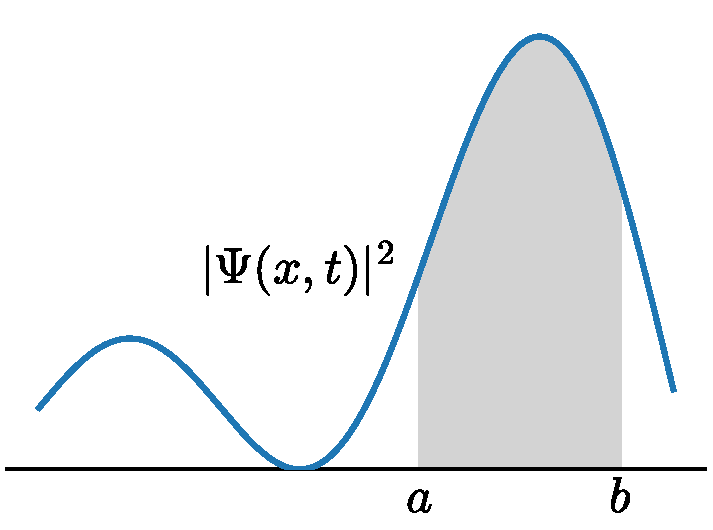
\includegraphics[width=0.4\linewidth]{prob-density}
	\caption{A plot of the absolute square of $\Psi$, with the shaded area representing the probability of finding the particle between points $a$ and $b$.}
	\label{fig:wfprob}
\end{figure}

The statistical interpretation is helpful for many reasons. For one, Equation~\ref{eq:wfprob} helps us reconcile our observations of discrete particles with the continuous nature of the wave function by modeling the latter as a probability. Taking the modulus squared of the wave function also results in a real quantity, since it is equivalent to multiplying the complex wave function by its complex conjugate.
\begin{tcolorbox}[title=Key point: modulus squared of a complex number] \vspace{-2ex}
	\begin{equation}
		\abs{\Psi}^2 = \Psi^*\Psi
	\end{equation}
\end{tcolorbox}

Like any good quantum theory, this interpretation has some strange consequences, the most significant of which is the idea of \textbf{indeterminacy}.\footnote{For a dense read perfect for a Friday evening, check out B. d'Espagnat, \href{https://www.scientificamerican.com/media/pdf/197911_0158.pdf}{\emph{Scientific American}} \textbf{11}, (1979), 158-181.} Notice that we cannot be certain about making measurements of position at the quantum scale, but we can only give a statistical figure as to the \emph{probability} of that result being measured. This is particularly troublesome if a measurement has been made of a particle's position, and then you ask where the particle was \emph{right before} the measurement was made. Was the particle at the same position where you had measured it? If so, why does quantum mechanics still give the possibility, however slight, that it was in fact meters away? And if it wasn't right there, where exactly was the particle?\footnote{\href{http://physicstoday.scitation.org/doi/abs/10.1063/1.880968}{Is the moon there when nobody looks?} N. Mermin, \emph{Physics Today} \textbf{38}, 4 (1985), 38-47.}

%%%%%%%%%%%%%%%%%%%%%%%%%%%%%%%%%%%%%%%%%%%%%%%%%%%%%%%%%%%%%%%%%%%%%%%%%%%%%%%%

\section{Normalization} \label{sec:normse}
However, even when we're surrounded by this uncertainty, there is one thing we \emph{can} be certain of---that \emph{somewhere} in space, the particle must exist and we can find it. This translates mathematically into 
\begin{tcolorbox}[title=Normalization condition] \vspace{-1ex}
	\begin{equation}
	\int_{-\infty}^{+\infty} \abs{\Psi(x,t)}^2 \dd{x} = 1 \label{eq:norm}
	\end{equation}
\end{tcolorbox}

This equation says that the particle is guaranteed to exist in our system at any point in time, which must hold true for the statistical interpretation to make sense. \par 

However, Equation~\ref{eq:norm} also imposes a constraint on the constant factor in the wave function, which we denoted with $A$ back in Equation~\ref{eq:propwave}. Specifically, we have
\begin{align*}
	\int_{-\infty}^{+\infty} \abs{\Psi(x,t)}^2 \dd{x} &= 1 \\
	\int_{-\infty}^{+\infty} \abs{A\Psi(x,t)}^2 \dd{x} &= 1 \\
	\abs{A}^2 \int_{-\infty}^{+\infty} \abs{\Psi(x,t)}^2 \dd{x} &= 1
\end{align*}

This process is called \textbf{normalizing} the wave function. Now we can define $A$ more precisely as a (possibly complex) coefficient that maintains the normalization condition in Equation~\ref{eq:norm}. Amazingly, the \Sch\ equation has the property that it preserves the normalization of the wave function over time, which means that we only have to solve for $A$ once!

%%%%%%%%%%%%%%%%%%%%%%%%%%%%%%%%%%%%%%%%%%%%%%%%%%%%%%%%%%%%%%%%%%%%%%%%%%%%%%%%

\section{Superposition} \label{sec:super}
One of the most important consequences of the \Sch\ equation is that it can correctly model the superposition principle we discussed back in Chapter 1. Recall how we observed in the Stern-Gerlach experiment that the silver atoms seemed to simultaneously exist in two quantum states, $\ket{S^+}$ and $\ket{S^-}$. Could this mean that there exist multiple wave functions that satisfy the \Sch\ equation and collectively describe the behavior of the particle? Absolutely! \par 

Specifically, if we have a wave function $\Psi_1$ that satisfies the \Sch\ equation and a second wave function $\Psi_2$ that also satisfies the \Sch\ equation, then \emph{any linear combination} of the two equations, $\Psi = c_1\Psi_1 + c_2\Psi_2$, is also a valid solution. You might be familiar with this property of linearity if you have already taken a course on differential equations. It allows us to take a set of all possible solutions to the \Sch\ equation and add them together to give a complete representation of all possible quantum states that the particle can be in. \par 

Mathematically, the linearity principle of differential equations provides an explanation for the superposition we previously observed. As improbable as it may have seemed before, we now have yet another reason to believe that particles are capable of simultaneously existing in multiple states. It turns out that we can generalize the result from above even further and decompose any wave function into a sum of distinct quantum states. This is expressed generally as
\begin{tcolorbox}[title=Superposition of wave functions] \vspace{-2ex}
	\begin{equation}
		\Psi = \sum_n c_n\Psi_n  \label{eq:super}
	\end{equation}
\end{tcolorbox}

This equation is the general form that you should keep in mind as we derive more specific instances of the wave function in the following chapters.\footnote{If you have taken a course like CME 104 or MATH 53 here at Stanford, Equation~\ref{eq:super} should seem suspiciously similar to a Fourier series decomposition. While we leave out much of the mathematical hairiness in this course, this is indeed the case, and you can consider the individual wave functions $\Psi_n$ to be eigenstates that form a basis for the space occupied by $\Psi$.}

\section[Time-independence]{Time-independent \Sch\ equation}
Now we will return to the original \Sch\ equation, which was given in Equation~\ref{eq:tdse} as
\begin{equation*}
	i\hbar \pdv{\Psi}{t} = -\frac{\hbar^2}{2m} \pdv[2]{\Psi}{x} + V(x,t)\Psi
\end{equation*}

This is a very complicated differential equation whose general solution is a function of two variables $x$ and $t$. We now consider a special case where the potential function is \emph{time-independent}, i.e. $V=V(x)$, such as that given by a stationary, external electric field. This allows us to apply \textbf{separation of variables} and guess that the solution can be written as a product of two separate functions, each of which is a function of only one variable:\footnote{There's unfortunately no good rationale for why it would occur for us do this, other than ``it's been attempted many times and works well.'' See \href{https://math.stackexchange.com/questions/575205/why-separation-of-variables-works-in-pdes}{math.stackexchange} for a discussion.} 
\begin{tcolorbox}[title = Separation of variables] \vspace{-2ex}
\begin{equation}
	\Psi(x,t) = \psi(x)\phi(t) \label{eq:sep}
\end{equation}
\end{tcolorbox}

Here, $\psi$ (lower-case ``psi'') is a function of $x$ alone, and $\phi$ (lower-case ``phi'') is a function of $t$ alone. This huge simplification allows us to derive a set of interesting solutions that in many cases model quantum mechanical states quite well. Moreover, we've seen in the previous section (Equation~\ref{eq:super}) that it's still possible to superimpose the separable solutions to construct the general solution to the \Sch\ equation. \par

The assumption of time-independent potentials turns the partial differential equation into two ordinary differential equations. We can substitute Equation~\ref{eq:sep} into the \Sch\ equation to obtain
\begin{align*}
	i\hbar \pdv{\Psi}{t} &= -\frac{\hbar^2}{2m} \pdv[2]{\Psi}{x} + V(x,t)\Psi \\
	i\hbar\psi \dv{\phi}{t} &= -\frac{\hbar^2}{2m} \phi\dv[2]{\psi}{x} + V(x)\psi(x)\phi(t) \tag{note the ordinary derivatives now} \\
	i\hbar\frac{1}{\phi} \dv{\phi}{t} &= -\frac{\hbar^2}{2m} \frac{1}{\psi}\dv[2]{\psi}{x} + V(x) \numberthis \label{eq:const}
\end{align*}

Now observe that the left hand side of Equation~\ref{eq:const} is purely a function of $t$ and the right hand side is purely a function of $x$. The only way this equation can be satisfied is if both sides are equal to a \emph{constant} (otherwise, you could vary one side without varying the other by just changing one variable). Let's call this constant $E$, for \textbf{energy}, and we will see why below. In any case, this gives us two equations, one for the left hand side,
\begin{equation}
	i\hbar \dv{\phi}{t} = E\phi \label{eq:phi}
\end{equation}
and another for the right hand side,
\begin{equation}
	-\frac{\hbar^2}{2m} \dv[2]{\psi}{x} + V(x)\psi = E\psi \label{eq:tise}
\end{equation}

Equation~\ref{eq:phi} can be solved using fairly straightforward integration. Specifically, we obtain
\begin{align*}
	i\hbar \dv{\phi}{t} &= E\phi \\
	\int \frac{1}{\phi} \dd{\phi} &= \int -\frac{iE}{\hbar} \dd{t} \\
	\ln \phi &= -\frac{iEt}{\hbar} \\ 
	\Aboxed{\phi(t) &= Ae^{-iEt/\hbar}} \numberthis
\end{align*}
which is another complex exponential function. Equation~\ref{eq:tise}, on the other hand, cannot be solved unless $V(x)$ is specified. In fact, this equation is formally known as the \textbf{time-independent \Sch\ equation} and it can be solved for a variety of simple potentials $V(x)$.
\begin{tcolorbox}[title = Time-independent \Sch\ equation] \vspace{-2ex}
	\begin{equation*}
		-\frac{\hbar^2}{2m} \dv[2]{\psi}{x} + V(x)\psi = E\psi
	\end{equation*}
\end{tcolorbox}

Overall, the solution we have found to Equation~\ref{eq:sep} is
\begin{equation}
	\Psi(x,t) = \psi(x)e^{-iEt/\hbar}
\end{equation}
where we have absorbed the constant $A$ into $\psi(x)$, the solution to the time-independent \Sch\ equation. Here are some further remarks and analyses of the general time-independent solution.
\begin{enumerate}[1.]
	\item The solutions $\psi(x)$ are called \textbf{stationary states} because the probability density is no longer time-dependent. Observe that 
	\begin{equation*}
		\abs{\Psi(x,t)}^2 = \abs{\psi(x)e^{-iEt/\hbar}}^2 = \abs{\psi(x)}^2e^{-iEt/\hbar}e^{iEt/\hbar} = \abs{\psi(x)}^2e^0 = \abs{\psi(x)}^2
	\end{equation*}
	and the time-dependence cancels out. This suggests that nothing is ``occurring'' in a stationary state since the probability of finding a particle does not change with time.
	
	\item Let's go back and address why we labeled the unknown constant as $E$ for energy. Recall that we argued in class that the energy in quantum mechanics could be represented by an \textbf{operator} 
	\begin{equation}
		\hat{E} = i\hbar\pdv{t} \label{eq:Eop}
	\end{equation}
	
	and the momentum by another operator 
	\begin{equation}
		\hat{p} = -i\hbar\pdv{x} \label{eq:Pop}
	\end{equation}
	
	Operators can be considered as special functions that map between different physical states and we distinguish them from their classical values with a hat symbol. Viewed in this way, we see that the time-independent \Sch\ equation is just a statement that the total energy is given by the sum of the kinetic energy and the potential energy. It is reassuring to see that conservation of energy also applies at the quantum level! In fact, this sum is another operator in and of itself, known as the \textbf{Hamiltonian},
	\begin{tcolorbox}[title = Hamiltonian operator] \vspace{-2ex}
		\begin{equation}
		\hat{H} = -\frac{\hbar^2}{2m}\pdv[2]{x}+V(x) \label{eq:ham}
		\end{equation}
	\end{tcolorbox}
	which allows us to write the time-independent \Sch\ equation as
	\begin{equation}
		\hat{H}\psi = E\psi \label{eq:tise-ham}
	\end{equation}
	
	Conveniently, the time-independent \Sch\ equation expressed in this form shows that stationary states have a single \emph{definite energy} that is invariant with respect to time, instead of a superposition of different energies. We will definitely see the Hamiltonian again in later chapters.
	
	\item Last but not least, we note that we have a solution for finding \emph{a particular} solution, but not the general solution. As alluded to in the previous section, we can actually find a set of solutions labeled by an index $n$. Due to the superposition principle, we can construct the general solution to the time-dependent \Sch\ equation\footnote{Note our language here: Superposition states \emph{cannot} be a solution to the time-\emph{independent} \Sch\ equation anymore, as each term would have a different energy value.} as a quantum superposition state given by
	\begin{tcolorbox}[title = Superposition of states] \vspace{-2ex}
		\begin{equation}
		\Psi(x,t) = \sum_{n=1}^{\infty} A_n\psi_n(x)e^{-iE_nt/\hbar} \label{eq:tise-sup}
		\end{equation}
	\end{tcolorbox}
	Now all that remains is to find the coefficients $A_n$, which we will see how to do in the following chapter. Once that is complete, we can construct the general solution to the \Sch\ equation using Equation~\ref{eq:tise-sup} and a (possibly infinite) set of stationary states as the basis.
\end{enumerate}

%%%%%%%%%%%%%%%%%%%%%%%%%%%%%%%%%%%%%%%%%%%%%%%%%%%%%%%%%%%%%%%%%%%%%%%%%%%%%%%%

\section[\Sch's Cat]{Application: \Sch's Cat}
We end this chapter with an entertaining discussion about a famous consequence of the \Sch\ equation and the principle of superposition. Shortly after \Sch\ published his namesake wave equation, Niels Bohr and Werner Heisenberg devised the \textbf{Copenhagen interpretation} of quantum mechanics,\footnote{A history of its development is provided by the \href{http://history.aip.org/exhibits/heisenberg/p09.htm}{American Institute of Physics}.} which states among many other things that \emph{prior} to making a \textbf{measurement}, a quantum system exists without definite properties, i.e. in a superposition state; it is only in the \emph{process} of making a measurement that the superposition of wave functions is disturbed and \textbf{collapses} into one of the possible states. \par 

While this novel interpretation was groundbreaking, many notable scientists did not agree, chief among them Einstein and \Sch. For his entire life, Einstein had trouble reconciling the Copenhagen interpretation with everyday reality and asserted in a 1935 landmark publication that the wave function was incomplete.\footnote{A. Einstein, B. Podolsky, N. Rosen. \href{https://journals.aps.org/pr/abstract/10.1103/PhysRev.47.777}{\emph{Phys. Rev.}} \textbf{47}, 777 (1935)} As is typically done in a field like quantum mechanics, Einstein formulated a hypothetical paradox in a \textbf{thought experiment} (\emph{Gedankenexperiment} in German) to show the shortcomings of the Copenhagen interpretation. \par 

\begin{figure}[!h]
	\centering
	\includegraphics[width=0.55\linewidth]{cat}
	\caption{\Sch's cat thought experiment. Radioactive decay, which happens at random, will cause the flask to shatter and release the poison, which kills the cat. While classical observation says the cat is alive \emph{or} dead, the Copenhagen interpretation says the cat is \emph{simultaneously} alive \emph{and} dead prior to observation. Image courtesy of \href{https://en.wikipedia.org/wiki/Schrödinger\%27s_cat}{Wikipedia}.}
	\label{fig:cat}
\end{figure}

While the details of the aforementioned EPR paradox will be left as an exercise to the reader, another thought experiment that illustrated the problem of the Copenhagen interpretation quite well was \textbf{\Sch's cat}, formulated by its namesake in response to Einstein's article. Shown here in Figure~\ref{fig:cat}, \Sch\ proposed a situation where a cat is trapped in a steel chamber with a radioactive substance that randomly decays over time. When it decays, a hammer is released to break a flask of poison which then kills the cat. However, we will not know the outcome until we open the steel chamber some time later, and only then can we confirm if the cat is alive or dead. Just like the question we posed at the end of Section~\ref{sec:prob}, what then, is the state of the cat at any point in time \emph{before} the observation is made? \par

If the Copenhagen interpretation was extended to the macroscopic world, then the cat must be in a superposition of states while inside the sealed chamber, which effectively makes it simultaneously alive \emph{and} dead. But this is directly contrary to the classical description, which says that the cat can only be alive \emph{or} dead. Is one set of laws ``more correct'' than the other? \par 

It turns out there's no single, accepted answer to this paradox, and I encourage you to think through its peculiarities. Ultimately, \Sch\ was interested in seeing when a quantum state transitions from a superposition of states into a unique classical state. This actually has profound consequences on what it means to make an \textbf{observation/measurement} of a quantum mechanical system and how scientists are inherently limited in the accuracy of their measurements by the strange laws of quantum mechanics.

%%%%%%%%%%%%%%%%%%%%%%%%%%%%%%%%%%%%%%%%%%%%%%%%%%%%%%%%%%%%%%%%%%%%%%%%%%%%%%%%

\section{Summary}
\begin{figure}[!h]
	\centering
	\includegraphics[width=0.9\linewidth]{xkcd-schrodinger}
	\caption{Image courtesy of \href{https://xkcd.com/45/}{xkcd}.}
	\label{fig:xkcd2}
\end{figure}

To recap, we started this chapter searching for a mathematical expression that could describe the wave-like behavior of particles that we observed in the previous chapter. We saw how Erwin \Sch's namesake wave equation did just that, and we used a time-independent potential function to simplify its overall formulation from a time-dependent, linear partial differential equation (Equation~\ref{eq:tdse}) into a time-independent, linear ordinary differential equation (Equation~\ref{eq:tise}). However, our focus was less on the math and more on the analysis of the wave function $\Psi$, where we saw how the statistical interpretation, normalization condition, and superposition principle all helped us make sense of the solutions to the \Sch\ equation. Even though scientists continue to debate the interpretation of the \Sch\ equation, there is no debate over its power, which we will utilize in the next chapter when we consider the particle in a box model. I assure you---the fun has only just begun!


%} % for doublespacing
%\end{document}	% The Schrodinger equation

% Created: Enze Chen, June 2017

% Chapter 3 of the MSE 142 coursereader. 
% This chapter discusses the particle in a box model as a concrete application of the time-independent Schrodinger equation. 
% Quantization, normalization, and the uncertainty principle are discussed. 
% This model is a good approximation for quantum dots, our first physical example of a quantum mechanical system.

% Uncomment the following three lines and last line to individually compile this chapter
%\documentclass[12pt, english]{book}
%\usepackage{142crstyle}
%\begin{document}

\chapter{Particle in a Box} \label{ch:box}
%{ \doublespacing 

In the previous chapter, we derived the \Sch\ equation, which provides the theoretical underpinning for all quantum mechanical calculations. 
Now we will apply the \Sch\ equation to a canonical example and solve for the wavefunction $\Psi(x,t)$. 
This will give us a better understanding of the mathematical constructs we saw previously and how they can be applied to a physical system like quantum dots.


% % % % % % % % % % % % % % % % % % % % % % % % % % % % % % % % % % % % % 
% % % % % % % % % % % % % % % % % % % % % % % % % % % % % % % % % % % % % 
% % % % % % % % % % % % % % % % % % % % % % % % % % % % % % % % % % % % % 
\section{Before you begin}

This chapter builds on the following concepts, some of which we've already discussed in class, others you will likely have encountered elsewhere.
We include links to resources that may aid your review, as mastery of these concepts will allow you to get the most out of this chapter.

\begin{itemize}
	\item foo
\end{itemize}

\begin{tcolorbox}[colframe=PaloAlto, colbacktitle=PaloAlto!20!white, title=Pre-check quiz]
	We strongly recommend everyone to take \href{TODO}{the autograded quiz} for this chapter \emph{before} you begin.
	It is anonymous and doesn't affect your grade, but it will give you some feedback and situate you for what's about to come.
\end{tcolorbox}


% % % % % % % % % % % % % % % % % % % % % % % % % % % % % % % % % % % % % 
% % % % % % % % % % % % % % % % % % % % % % % % % % % % % % % % % % % % % 
% % % % % % % % % % % % % % % % % % % % % % % % % % % % % % % % % % % % % 
\section{Formulation}

As its name would imply, the \textbf{particle in a box} model is just that: we have a small particle (e.g., an electron) that is free to move (in one dimension) in a small space confined between $x = 0$ and $x = L$ (\autoref{fig:box}). 
In order to keep the particle confined, we imagine the potential $V$ to be $\infty$ outside of the walls and 0 on the inside. 
For this reason, this model is also known as the \textbf{infinite potential well}.\footnote{FYI: what is the ``box."}
Physically, you can think of this as a guitar string of length $L$ with the two ends fixed in place so that it cannot vibrate at the ends.

\begin{figure}[!h]
	\centering
	\includegraphics[width=0.45\linewidth]{particle-in-a-box.pdf}
	\caption{Particle in a box model. 
		The potential $V(x)$ is zero for $x \in [0,L]$ and infinite everywhere else, which confines the movement of the particle to be inside the walls at all times.}
	\label{fig:box}
\end{figure}

The particle in a box model is a great starting point for us because it can be solved analytically to illustrate all sorts of amazing quantum behavior. 
We first enforce the condition that the wavefunction $\Psi(x,t)$ must be zero at $x = 0$ and $x = L$ for all time $t$. 
This means the probability of finding the particle there is zero, which makes sense given the infinite potential barriers.

Inside the box, where $V(x) = 0$, the time-independent \Sch\ equation (\autoref{eq:tise}) now adopts a simplified form:

\begin{tcolorbox}[title=\Sch\ equation for particle in a box] \vspace{-2ex}
	\begin{equation}
		-\frac{\hbar^2}{2m} \dv[2]{\psi_n}{x} = E_n\psi_n  \label{eq:box-se}
	\end{equation}
\end{tcolorbox}

\noindent where we have again explicitly put the index $n$ to label different solutions for different quantum states. 
Now we are looking for a function with which two derivatives will give us back the original function times a negative constant. 
\autoref{eq:box-se} is actually the equation for a simple harmonic oscillator from classical mechanics, which you might recall has sines and cosines as solutions.\footnote{Alternatively, employ the method of educated guessing as we showed in class to arrive at this result.} 
In fact, the general solution is given by 

\begin{tcolorbox}[title=General solution to particle in a box] \vspace{-2ex}
	\begin{equation}
		\psi_n(x) = A\sin(k_nx) + B\cos(k_nx) \label{eq:box-gensol}
	\end{equation}
\end{tcolorbox}

\noindent where $k_n = \sqrt{2mE_n/\hbar^2}$ and $A$ and $B$ are arbitrary constants. 
We definitely took a big jump going directly from \autoref{eq:box-se} to \autoref{eq:box-gensol}, so if you're not quite convinced, I recommend plugging the latter equation into the former to make sure that it is indeed a valid solution.


% % % % % % % % % % % % % % % % % % % % % % % % % % % % % % % % % % % % % 
% % % % % % % % % % % % % % % % % % % % % % % % % % % % % % % % % % % % % 
% % % % % % % % % % % % % % % % % % % % % % % % % % % % % % % % % % % % % 
\section{Quantization}

With the general solution on hand, we now look to see if the constraints in the problem can help us simplify some of the constants. 
Typically, the constants that appear in solutions to differential equations are fixed by the \textbf{boundary conditions} of the problem. 
We already noted earlier that

\begin{align}
	\psi(0) &= 0 \\
	\psi(L) &= 0
\end{align}

\noindent which seem appropriate for this model. 
From the first boundary condition, we have

\begin{equation*}
	\psi(0) = A\sin(k_n \cdot 0) + B\cos(k_n \cdot 0) = B = 0
\end{equation*}

\noindent which means the cosine term is eliminated! 
From the second boundary condition, we have

\begin{equation*}
	\psi(L) = A\sin(k_nL) = 0
\end{equation*}

This scenario is slightly trickier, but realize that we cannot have $A = 0$ and still have a physically meaningful solution, so we must have $\sin(k_nL) = 0$. 
Since the sine function has roots at integer multiples of $\pi$, this means that

\begin{equation}
	k_nL = 0,\ \pm\pi,\ \pm2\pi,\ \pm3\pi,\ \dots \label{eq:k-pi-box}
\end{equation}

Analyzing \autoref{eq:k-pi-box} closely, we can argue that $k = 0$ would also lead to a trivial solution and we can eliminate the negative solutions due to symmetry.\footnote{Given that $\sin(-k_nL) = -\sin(k_nL)$, we would obtain the same wavefunction up to a sign.} 
Therefore, it must be the case that 

\begin{tcolorbox}[title=Allowed values of $k$] \vspace{-2ex}
	\begin{equation}
		k_n = \frac{n\pi}{L}, \quad n = 1, 2, 3, \dots   \label{eq:k-box}
	\end{equation}
\end{tcolorbox}

Now you see why we chose to index the solutions with the subscript $n$ all along. 
Furthermore, because $k_n = \sqrt{2mE_n/\hbar^2}$, we can use some algebra and find that

\begin{tcolorbox}[title = Allowed energies] \vspace{-2ex}
	\begin{equation}
		E_n = \frac{\hbar^2n^2\pi^2}{2mL^2} \label{eq:E-box}
	\end{equation}
\end{tcolorbox}

The results from these two expressions show that the energy states of a particle in an infinite potential well are not a continuum of values but rather a set of discrete energy levels. 
Thus we say that the energies for a particle in a box are \textbf{quantized}, where each state is indexed by the \textbf{quantum number} $n$. 
We see then that $n = 1$ corresponds to the lowest energy state, called the \textbf{ground state} of the system, and higher energy states are called \textbf{excited states} (analogous to harmonics in music). 
Note how strange this is: Whereas classically, a particle can have zero total energy, here we are saying that is not the case, even for the ground state!\footnote{We will elaborate on this further in \autoref{ch:qho} when we discuss the zero-point energy of the quantum harmonic oscillator.} 


% % % % % % % % % % % % % % % % % % % % % % % % % % % % % % % % % % % % % 
% % % % % % % % % % % % % % % % % % % % % % % % % % % % % % % % % % % % % 
% % % % % % % % % % % % % % % % % % % % % % % % % % % % % % % % % % % % % 
\section{Normalization}

Now that we have an expression for $k_n$ and cleverly eliminated $B$, all that's left is to find the leading coefficient $A$. 
Recall how in \autoref{sec:normse} we used the normalization condition to help us with this task, so let's apply that again here. 
Specifically, we have

\begin{align*}
	\int_0^L \abs{A}^2 \sin^2(k_nx)\dd{x} &= 1 \\
	\abs{A}^2 \int_0^L \sin^2\left(\frac{n\pi x}{L}\right)\dd{x} &= 1 \\ 
	\abs{A}^2 \int_0^L \frac{1}{2} - \frac{1}{2}\cos\left(\frac{2n\pi x}{L}\right)\dd{x} &= 1 \\
%	\abs{A}^2 \left( \frac{L}{2} - \frac{L}{4n\pi}(\sin(2n\pi) - \sin(0)) \right) &= 1 \\
	\abs{A}^2 \left(\frac{L}{2}\right) &= 1 \\
	\abs{A}^2 &= \frac{2}{L}
\end{align*}

\noindent where we have used the trigonometric identity $\sin^2(x) = \frac{1}{2} \left( 1 - \cos(2x) \right)$ going from the second line to the third line. 
We take the positive real root to get $A = \sqrt{2/L}$. 
Inside the confines of the box, we have the stationary state solutions given by:

\begin{tcolorbox}[title=Stationary state solutions] \vspace{-2ex}
	\begin{equation}
		\psi_n(x) = \sqrt{\frac{2}{L}} \sin \left(\frac{n\pi x}{L}\right) \label{eq:box-ss}
	\end{equation}
\end{tcolorbox}

The first three stationary states are plotted in \autoref{fig:ss-box}, and they look similar to the standing waves we observe when we pluck a guitar string.\footnote{In fact, the superposition of the various harmonics in musical instruments is what gives each instrument its unique timbre, or tone quality.} 
We will call zero-crossings on the wavefunction \textbf{nodes}, which means the $n^{\text{th}}$ quantum state has $n - 1$ nodes (alternatively, the $n^{\text{th}}$ \emph{excited state} has $n$ nodes). 
These nodes restrict the location where the particle may be found and contribute to the symmetry of the wavefunctions.

\begin{figure}[!h]
	\centering
	\subfloat[]{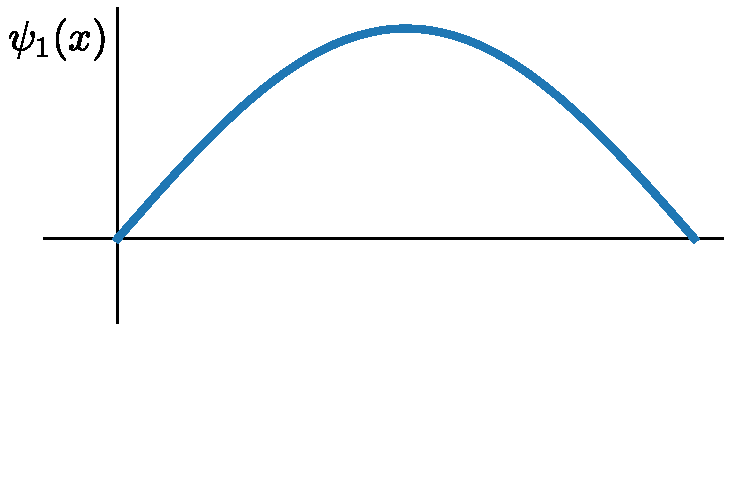
\includegraphics[width=0.33\linewidth]{ss-1.pdf}}
	\subfloat[]{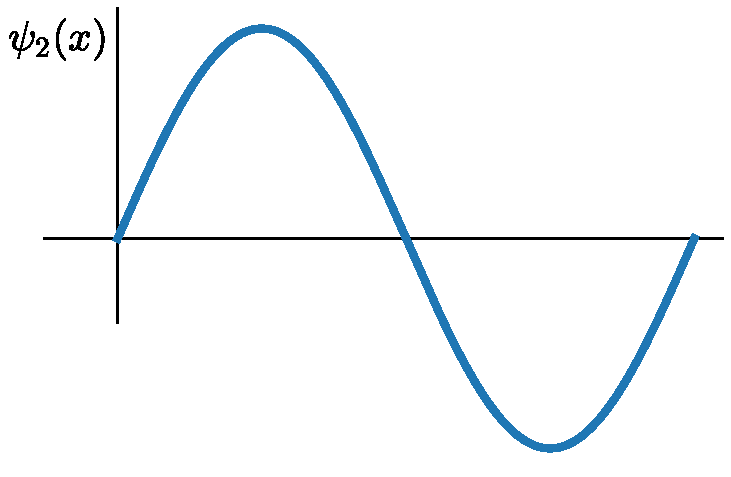
\includegraphics[width=0.33\linewidth]{ss-2.pdf}}
	\subfloat[]{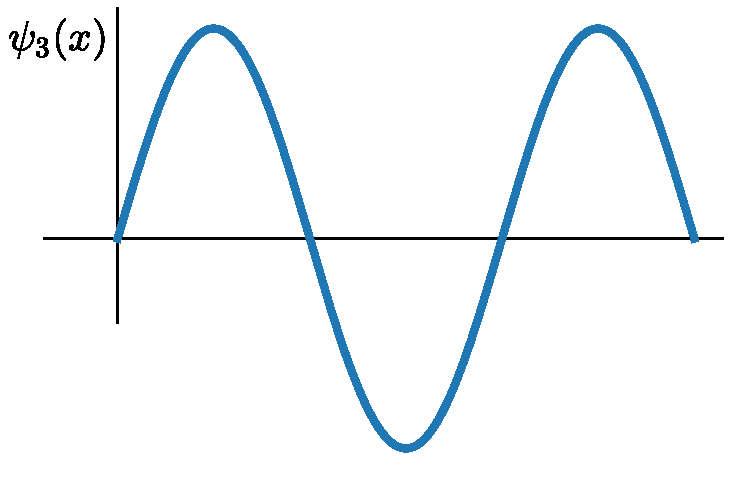
\includegraphics[width=0.33\linewidth]{ss-3.pdf}}
	\caption{The first three stationary states of the particle in a box model.}
	\label{fig:ss-box}
\end{figure}


% % % % % % % % % % % % % % % % % % % % % % % % % % % % % % % % % % % % % 
% % % % % % % % % % % % % % % % % % % % % % % % % % % % % % % % % % % % % 
% % % % % % % % % % % % % % % % % % % % % % % % % % % % % % % % % % % % % 
\section{Orthogonality}

Another interesting property of the wavefunctions given by \autoref{eq:box-ss} is that they are all mutually orthogonal. 
This means 

\begin{equation*}
	\int \psi_m^*(x) \psi_n(x) \dd{x} = 0, \quad \forall m \neq n
\end{equation*}

\noindent where $\psi^*$ again denotes the complex conjugate. 
We will show this as follows:

\begin{align*}
	\int \psi_m^*(x) \psi_n(x) \dd{x} &= \frac{2}{L} \int_0^L \sin\left(\frac{m\pi x}{L}\right) \sin\left(\frac{n\pi x}{L} \right) \dd{x} \\
	&= \frac{1}{L} \int_{0}^{L} \left[ \cos\left(\frac{(m-n)\pi x}{L}\right) - \cos\left(\frac{(m+n)\pi x}{L}\right) \right] \dd{x} \\
	&= \left[ \frac{1}{(m-n)\pi} \sin \left(\frac{(m-n)\pi x}{L}\right) - \frac{1}{(m+n)\pi} \sin\left( \frac{(m+n)\pi x}{L} \right)\right] \bigg|_0^L \\
	&= \frac{1}{\pi} \left( \frac{\sin((m-n)\pi)}{m-n} - \frac{\sin((m+n)\pi)}{m+n}\right) \\
	&= 0 \tag{when $m\neq n$, $\{m,n\} \in \mathbb{Z}$}
\end{align*}

\noindent where we used the identity $\sin(m)\sin(n) = \frac{1}{2}(\cos(m - n) - \cos(m + n))$ in the second line. 
That's pretty neat! 
We do note, however, the special case when $m=n$. 
In that case, by the normalization condition, the integrand is equivalent to the probability density function, which we know equals 1 when integrated over the range of $x$. 
This fact allows us to combine orthogonality and normalization into a single expression.

\begin{tcolorbox}[title = Orthonormal stationary states] \vspace{-2ex}
	\begin{equation}
		\int \psi_m^*(x) \psi_n(x) \dd{x} = \delta_{mn}\ \begin{cases}
		1 & \text{if}\ m=n \\
		0 & \text{if}\ m\neq n
		\end{cases} \label{eq:orthonorm}
	\end{equation}
\end{tcolorbox}

\noindent where $\delta_{mn}$ is known as the \textbf{Kronecker delta} function. 
Now we have confirmed that the $\psi$'s form an \textbf{orthonormal basis}, which allows us to express \emph{any} function as a linear combination of them.\footnote{I wanted correctness here, but this is excessive linear algebra jargon. A common example of an orthonormal basis is the set of unit vectors $\mathbf{i}$, $\mathbf{j}$, $\mathbf{k}$ in $(x,y,z)$ coordinates. Every point in 3D space is some linear combination of the three unit vectors and each unit vector is orthogonal to the others.} 
Thus, we can write down the full, time-dependent solution for the particle in a box as:

\begin{equation}
	\Psi(x,t) = \sum_{n=1}^{\infty} A_n \sin \left(\frac{n\pi x}{L}\right) e^{-iE_nt/\hbar} \label{eq:tdwf-box}
\end{equation}

This equation gets us very close to the general solution, but we still have $A_n$ to solve for---and that's where the following ``mathematical trick'' comes in. 
We noted in \autoref{sec:normse} how $A_n$ is time-invariant, so let's look at our wavefunction at time $t = 0$. 
From \autoref{eq:tdwf-box}, we obtain

\begin{equation*}
	\Psi(x,0) = \sum_{n=1}^{\infty} A_n \sin \left(\frac{n\pi x}{L} \right)
\end{equation*}

\noindent where the exponential term has dropped out. 
Now for the ``trick'': It would appear that this is still an infinite sum of sine terms, but we can make use of \autoref{eq:orthonorm} by multiplying both sides by an arbitrary function $\sin \left(\frac{j\pi x}{L}\right)$ and then integrating the result.\footnote{This is definitely \emph{not} obvious, and is a technique borrowed directly from Fourier series (see \href{http://tutorial.math.lamar.edu/Classes/DE/FourierSeries.aspx}{Paul Dawkins'} page if you're curious). You don't need to know this trick per se, but do understand why it works (i.e., \autoref{eq:orthonorm}).} 
This gives us:

\begin{align*}
	\Psi(x,0) &= \sum_{n=1}^{\infty} A_n \sin \left(\frac{n\pi x}{L} \right) \\
	\Psi(x,0) \sin \left(\frac{j \pi x}{L}\right) &= \sum_{n=1}^{\infty} A_n \sin \left(\frac{n\pi x}{L} \right) \sin \left( \frac{j \pi x}{L}\right) \\
	\int_0^L \Psi(x,0) \sin \left(\frac{j \pi x}{L}\right) \dd{x} &= \int_0^L \sum_{n=1}^{\infty} A_n \sin \left(\frac{n\pi x}{L} \right) \sin \left( \frac{j \pi x}{L}\right) \dd{x} \\
	\int_0^L \Psi(x,0) \sin \left(\frac{j \pi x}{L}\right) \dd{x} &= \sum_{n=1}^{\infty} A_n \int_0^L \sin \left(\frac{n\pi x}{L} \right) \sin \left( \frac{j \pi x}{L}\right) \dd{x} \\
	\int_0^L \Psi(x,0) \sin \left(\frac{j \pi x}{L}\right) \dd{x} &= \sum_{n=1}^{\infty} A_n \delta_{nj} \frac{L}{2}
\end{align*}

The right hand side is 0 for all values of $n$ except when $n = j$. 
Thus the summation is eliminated(!) and we can move $\frac{L}{2}$ to the other side (and change $j$ to $n$) to obtain

\begin{tcolorbox}[title = Wavefunction expansion coefficients] \vspace{-2ex}
	\begin{equation}
		A_n = \frac{2}{L} \int_0^L \Psi(x,0) \sin \left(\frac{n\pi x}{L}\right) \dd{x} \label{eq:wf-coeff}
	\end{equation}
\end{tcolorbox}

Whew! After some nifty math, we were finally able to derive a general solution to the \Sch\ equation given the stationary state solutions from our particle in a box model. 
The general solution is given by \autoref{eq:tdwf-box} and those coefficients $A_n$ are described by \autoref{eq:wf-coeff} provided we are given some initial condition $\Psi(x,0)$.


% % % % % % % % % % % % % % % % % % % % % % % % % % % % % % % % % % % % % 
% % % % % % % % % % % % % % % % % % % % % % % % % % % % % % % % % % % % % 
% % % % % % % % % % % % % % % % % % % % % % % % % % % % % % % % % % % % % 
\section{Uncertainty principle}

Let's try to calculate the amplitude coefficients using \autoref{eq:wf-coeff} for a different case and arrive at another fundamental principle in quantum mechanics. 
First, we assume that our wavefunction has the initial profile shown in \autoref{fig:square-box}. 
That is, it is a square wave of height $A$ and width $b$ centered in the middle of the infinite potential well.

\begin{figure}[!h]
	\centering
	\includegraphics[width=0.26\linewidth]{square-box.pdf}
	\caption{Initial wavefunction profile of height $A$ and width $b$ centered in the middle of the well.}
	\label{fig:square-box}
\end{figure}

We directly crank through the calculations in \autoref{eq:wf-coeff} to obtain:

\begin{align*}
	A_n &= \frac{2}{L} \int_0^L \Psi(x,0) \sin \left(\frac{n\pi x}{L}\right) \dd{x} \\
	&= \frac{2A}{L} \int_{(L-b)/2}^{(L+b)/2} \sin \left(\frac{n\pi x}{L}\right) \dd{x} \\
	&= -\frac{L}{n\pi}\frac{2A}{L} \cos\left(\frac{n \pi x}{L}\right)\bigg|_{(L-b)/2}^{(L+b)/2} \\
	&= \frac{2A}{n\pi} \left[ \cos \left(\frac{L-b}{2}\frac{n\pi}{L}\right) - \cos \left(\frac{L+b}{2}\frac{n\pi}{L}\right) \right] \\
	&= \frac{4A}{n\pi} \sin \left(\frac{n\pi}{2}\right) \sin \left(\frac{n\pi b}{2L}\right) \\
	&= \frac{4A}{n\pi} (-1)^{\frac{n-1}{2}} \sin \left(\frac{n\pi b}{2L}\right) \tag{for odd $n$} \\
	&= \frac{4A(b/2L)}{n\pi(b/2L)} (-1)^{\frac{n-1}{2}} \sin \left(\frac{n\pi b}{2L}\right) \\
	\Aboxed{A_n &= \frac{2Ab}{L} (-1)^{\frac{n-1}{2}} \frac{\sin \left(k_nb/2\right)}{k_nb/2}} \numberthis \label{eq:A-example}
\end{align*}

Notice how we used the same trigonometric identity as before, $\sin(m)\sin(n) = \frac{1}{2}(\cos(m - n) - \cos(m + n))$, except backwards, when we went from the fourth line to the fifth line. 
The second to last line involves multiplying by ``1" so that we can get the final answer in the form of $\frac{\sin(x)}{x}$. 
This allows us to analyze \autoref{eq:A-example} in the form of a plot, which is shown in \autoref{fig:sinx/x}.

\begin{figure}[!h]
	\centering
	\includegraphics[width=0.35\linewidth]{sinx-x.pdf}
	\caption{A sketch of \autoref{eq:A-example}, which resembles the profile of $\frac{\sin(x)}{x}$. 
	The graph asymptotically approaches 0 and has zeros at the roots of $\sin(k_nb/2)$.}
	\label{fig:sinx/x}
\end{figure}

We observe in \autoref{fig:sinx/x} that the majority of the function (which we will gauge by the area under the curve) is contained within the first zero (black dot). 
We know from \autoref{eq:A-example} that this zero occurs when $\sin(k_nb/2)=0$; therefore,

\begin{equation}
	\frac{k_nb}{2} \ge \pi \implies k_n = \Delta k \ge \frac{2\pi}{b} \label{eq:delta-k}
\end{equation}

We will call the value $\Delta k$ the \textbf{uncertainty} in $k$, which we know by the de Broglie relation is related to momentum by $k=p/\hbar$. 
Notice that \autoref{eq:delta-k} also gives us an inverse relationship between $b$ and $\Delta k$; specifically, as $b \rightarrow 0$, $\Delta k \rightarrow \infty$, and vice versa. 

Now, what is $b$? 
Recall that it was the width of our initial wavefunction profile. 
When we vary $b$, what we're really doing is varying the width of our wavefunction, which we can effectively call $\Delta x$. 
We can combine these facts with the de Broglie relation (\autoref{eq:dBw}) to obtain

\begin{equation}
	p = \hbar k \implies \Delta p = \hbar \Delta k \ge  \frac{\hbar 2\pi}{b} = \frac{h}{\Delta x} \label{eq:up-almost}
\end{equation}

We can rearrange Equation~\ref{eq:up-almost} to obtain the final result:

\begin{tcolorbox}[title = Uncertainty principle] \vspace{-2ex}
	\begin{equation}
		\Delta p \Delta x \ge h \label{eq:up}
	\end{equation}
\end{tcolorbox}

This result, known as the \textbf{uncertainty principle},\footnote{The traditional formulation is given by: $\sigma_x\sigma_p \ge \hbar/2$, which relates standard deviations of position and momentum. A more rigorous proof is also given in the Griffiths textbook, Chapter 3.5.} establishes a fundamental property of quantum systems by stating that the more precisely a particle's momentum is determined (i.e. as $\Delta p$ gets smaller), the less precisely its position can be known (i.e. $\Delta x$ gets bigger), and vice versa. 
This relationship was first introduced in 1927 by Werner Heisenberg, so it is often known as \textbf{Heisenberg's uncertainty principle}.\footnote{W. Heisenberg, \href{https://doi.org/10.1007/BF01397280}{\emph{Z. Physik}} 43, 1927. For some historical context, see the \href{https://history.aip.org/exhibits/heisenberg/uncertainty-principle.html}{American Institute of Physics}.} 
The consequences of this theory troubled scientists initially,\footnote{Again, see the \href{http://history.aip.org/exhibits/heisenberg/}{American Institute of Physics}.} but it soon became clear that this uncertainty was an inherent property of all wave-like systems. 
It is also another example of the \textbf{complementarity} principle that was introduced at the end of \autoref{ch:intro}, and here it places a limit on the accuracy with which position and momentum can be simultaneously determined.


% % % % % % % % % % % % % % % % % % % % % % % % % % % % % % % % % % % % % 
% % % % % % % % % % % % % % % % % % % % % % % % % % % % % % % % % % % % % 
% % % % % % % % % % % % % % % % % % % % % % % % % % % % % % % % % % % % % 
\section{Application: Quantum dots}

The particle in a box model allowed us to derive some interesting properties at the nanoscale, and it turns out this approximation works very well when analyzing the behavior of \textbf{quantum dots}. 
Discovered in the early 1980s,\footnote{See L. E. Brus \href{http://aip.scitation.org/doi/abs/10.1063/1.447218}{\emph{J. Chem. Phys.}} 80, 1984; and more recently, the \href{https://www.nobelprize.org/prizes/chemistry/2023/summary/}{2023 Nobel Prize in Chemistry}.} quantum dots (QDs) are tiny semiconducting particles, only several nanometers in size, that confine their electrons such that they cannot escape, which makes the particle in a box model an apt comparison. 
This confinement allows the QD to emit specific frequencies of light when stimulated, which scientists are able to precisely tune by changing the dots' size, shape, and elemental composition (\autoref{fig:qdot}).

The small size of QDs form an infinite potential well that creates discrete electronic states similar to what we saw in this chapter. 
\autoref{eq:E-box} gave us the allowed energies for the particle in a box model as

\begin{equation*}
	E_n = \frac{\hbar^2n^2\pi^2}{2mL^2}
\end{equation*}

\noindent which can also be applied to QDs to determine the energy of the photons they emit during fluorescence. 
Note the dependence on the length scale $L$ in the previous equation. 
As $L$ becomes smaller and smaller, the allowed energies (and the spacing between energy levels) becomes larger and larger, which explains the changes in color observed in semiconductor QDs as their diameters are changed.

\begin{figure}[!h]
	\centering
	\includegraphics[width=0.35\linewidth]{quantum-dot.png} \\
	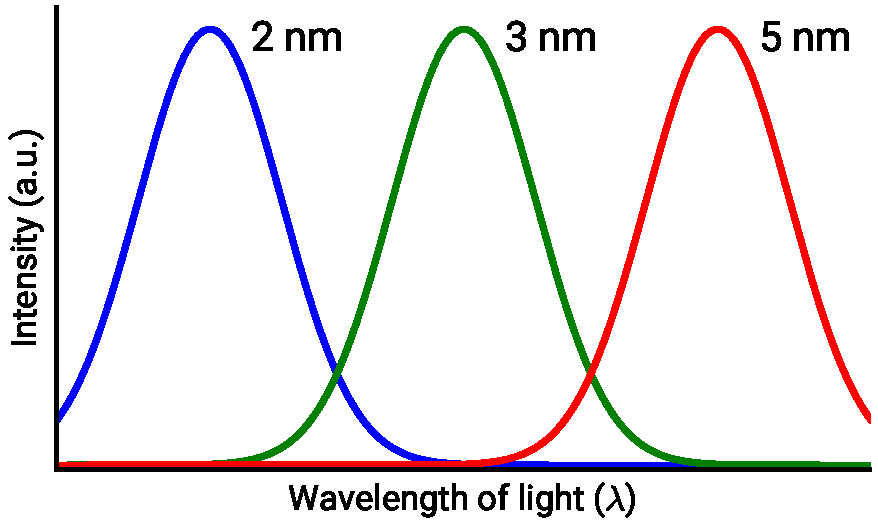
\includegraphics[width=0.42\linewidth]{quantum-dot-plot.pdf}
	\caption{The emission wavelength of cadmium selenide (CdSe) quantum dots can be tuned by changing the particle size. 
	Smaller QDs, with radii from 2--\SI{3}{\nano\meter}, turn blue and green, while QDs with larger radii $\sim\SI{5}{\nano\meter}$ appear red. 
	Top image reproduced from A. P. Alivisatos, \href{http://pubs.acs.org/doi/abs/10.1021/nn800485f1}{\emph{ACS Nano}} 2, 2008.}
	\label{fig:qdot}
\end{figure}

Because of their tunable properties, QDs see many potential applications in transistors, solar cells, LEDs, digital displays, medical imaging, and environmental monitoring.\footnote{There are many introductory articles out there on QDs, such as this editorial from \href{http://www.nature.com/nnano/journal/v5/n6/full/nnano.2010.127.html}{\emph{Nat. Nanotechnol.}} 5, 2010, and this article from J. Ouellette, \href{https://blogs.scientificamerican.com/cocktail-party-physics/quantum-dots-of-many-colors/}{\emph{Scientific American}}, 2012.} 
There's a lot of exciting research out there surrounding these nanoscale materials, whose functionality you should better understand having read this chapter!


% % % % % % % % % % % % % % % % % % % % % % % % % % % % % % % % % % % % % 
% % % % % % % % % % % % % % % % % % % % % % % % % % % % % % % % % % % % % 
% % % % % % % % % % % % % % % % % % % % % % % % % % % % % % % % % % % % % 
\section{Summary}

To recap, we dedicated this entire chapter to developing and analyzing the particle in a box quantum model. 
This simplistic, yet powerful assumption allowed us to solve the \Sch\ equation exactly, which revealed a set of stationary states and associated quantized energy levels. 
We demonstrated that the stationary state wavefunctions were orthogonal to each other, which allowed us to write the general solution to the \Sch\ equation as a superposition of stationary state solutions. 
We saw the complementarity of position and momentum manifest in the uncertainty principle, and we ended the chapter with a discussion of quantum dots, which are well-approximated by the particle in a box model. 
As we move on to more complex scenarios, we will be relaxing some of the strict assumptions we made in this chapter and exploring different potential functions. 
First, we will see what happens when we have a \emph{finite} potential barrier, which causes a peculiar phenomenon known as quantum tunneling.

%} % for doublespacing
%\end{document}	% Particle in a box

% Created: Enze Chen, June 2017
% Last edited: Enze Chen, February 2018
%
% Chapter 4 of the MSE 142 coursereader. This chapter discusses quantum tunneling using the finite potential step/barrier. It derives the math behind boundary conditions and tunneling probability. Interference from multiple boundaries is also discussed. There is an emphasis on applications to really drive the point home that this phenomenon is cool and more ubiquitous than we might initially think!

% Uncomment the following three lines and last line to individually compile this chapter
%\documentclass[12pt, english]{book}
%\usepackage{142crstyle}
%\begin{document}

\chapter{Quantum Tunneling} \label{ch:tunnel}
%{ \doublespacing 
Imagine you're tossing a tennis ball against the wall. Classical mechanics says that the ball will bounce back at you, or, should you throw it very hard, it might get stuck in the wall. But what if the ball somehow \emph{goes through} the wall and emerges on the other side, leaving both unscathed? This is the basis for \textbf{quantum tunneling}, a phenomenon where a particle passes through a potential barrier that it classically could not surmount. As bizarre as this may seem, quantum mechanics says there is a non-zero probability for tunneling to occur, and this phenomenon is actually leveraged for a variety of physical applications. Tunneling at the quantum scale occurs in physical systems ranging from photons\footnote{See D. D. Coon \href{http://aapt.scitation.org/doi/10.1119/1.1972893}{\emph{American Journal of Physics}} \textbf{34}, 240 (1966).} to water\footnote{See \href{https://physics.aps.org/articles/v9/43}{this focus article} from \emph{Physics} \textbf{9}, 43 about the work of A. I. Kolesnikov et al, \href{https://journals.aps.org/prl/abstract/10.1103/PhysRevLett.116.167802}{\emph{Physical Review Letters}} \textbf{116}, 167802 (2016).} and we will spend this chapter exploring the nature of this truly quantum mechanical behavior.

%%%%%%%%%%%%%%%%%%%%%%%%%%%%%%%%%%%%%%%%%%%%%%%%%%%%%%%%%%%%%%%%%%%%%%%%%%%%%%%%

\section{Finite potential step}
To facilitate our analysis of this behavior, we need to first devise a simple model for a quantum mechanical system, which we have shown here in Figure~\ref{fig:tunnel-step}. On the left half of the figure in region I, where $x < 0$, we have a free particle ($V=0$) traveling to the right with energy $E$. At $x=0$, the particle encounters a \textbf{potential step} with some \emph{finite} potential $V=V_0$ that extends for all $x>0$ into region II.

\begin{figure}[!h]
	\centering
	\includegraphics[width=0.42\linewidth]{tunnel-step}
	\caption{A simple model to demonstrate quantum tunneling. A free particle with energy $E$ is traveling to the right and at $x=0$ is incident on a finite potential step with magnitude $V_0$.}
	\label{fig:tunnel-step}
\end{figure}

Note that we have not said anything yet about the relationship between $E$ and $V_0$ (the vertical position of the particle in Figure~\ref{fig:tunnel-step} was arbitrarily drawn). Since the finite potential step is time-independent, we will try to understand how quantum mechanical particles interact with such a potential by solving the time-independent \Sch\ equation. In region I, we only have the free particle, so we can write down the \Sch\ equation as 
\begin{equation}
	-\frac{\hbar^2}{2m} \dv[2]{\Psi}{x} = E\Psi \label{eq:reg-1-se}
\end{equation}
In region II, we have
\begin{equation}
	-\frac{\hbar^2}{2m} \dv[2]{\Psi}{x} = (E-V_0)\Psi \label{eq:reg-2-se}
\end{equation}
where the energy of the particle is now with reference to the step's potential. We've seen these kinds of equations before and know that the general solution are sines and cosines, as was the case with the particle in a box. Here we write the general solutions in a slightly different, but equivalent way:
\begin{tcolorbox}[title = Traveling wave solutions] \vspace{-2ex}
	\begin{align}
		\Psi_{\text{I}} &= Ae^{ik_1x} + Be^{-ik_1x} \label{eq:reg-1-wf} \\
		\Psi_{\text{II}} &= Ce^{ik_2x} + De^{-ik_2x} \label{eq:reg-2-wf} 
	\end{align}
\end{tcolorbox}
where $A$, $B$, $C$, and $D$ are unknown coefficients. Whoa! We know by Euler's formula that complex exponentials can be reformulated as sinusoidal functions, so these solutions at least seem plausible on the surface. To be sure we did our math right, let's plug Equation~\ref{eq:reg-1-wf} into Equation~\ref{eq:reg-1-se} to verify that it is a valid solution.
\begin{align*}
	-\frac{\hbar^2}{2m} \dv[2]{\Psi_{\text{I}}}{x} &= E\Psi_{\text{I}} \\
	-\frac{\hbar^2}{2m} \dv[2]{x}(Ae^{ik_1x} + Be^{-ik_1x}) &= E(Ae^{ik_1x} + Be^{-ik_1x}) \\
	-\frac{\hbar^2}{2m} \dv{x}(Aik_1e^{ik_1x} - Bik_1e^{-ik_1x}) &= E(Ae^{ik_1x} + Be^{-ik_1x}) \\
	\frac{\hbar^2}{2m} \left(Ak_1^2e^{ik_1x} + Bk_1^2e^{-ik_1x}\right) &= E(Ae^{ik_1x} + Be^{-ik_1x}) \\
	k_1^2\left(Ae^{ik_1x} + Be^{-ik_1x}\right) &= \frac{2mE}{\hbar^2}(Ae^{ik_1x} + Be^{-ik_1x})
\end{align*}

So we see that
\begin{equation}
	k_1 = \sqrt{\frac{2mE}{\hbar^2}} \label{eq:reg-1-k}
\end{equation}
which is the same expression we found previously and shows that Equation~\ref{eq:reg-1-wf} is a valid solution. In a similar vein, we see that the magnitude of the wave vector in region II is given by 
\begin{equation}
	k_2 = \sqrt{\frac{2m(E-V_0)}{\hbar^2}} \label{eq:reg-2-k}
\end{equation}

Note that if $E > V_0$, then $k_2$ is real and we have sinusoidal behavior in region II. This makes sense because a particle with higher energy than the potential step should be able to surmount it and continue exhibiting wave-like behavior. However, if $E < V_0$, then $k_2$ becomes imaginary, and the wave-like solutions given in Equation~\ref{eq:reg-2-wf} turn into exponentially growing and decaying functions. Thus it seems like even though the particle does not have sufficient energy to surmount the potential step, there is still something happening in region II \emph{inside} the step. We will come back to this point shortly. \par 

%%%%%%%%%%%%%%%%%%%%%%%%%%%%%%%%%%%%%%%%%%%%%%%%%%%%%%%%%%%%%%%%%%%%%%%%%%%%%%%%

\section{Forward and backward waves}
Now, the general solutions given by Equation~\ref{eq:reg-1-wf} and~\ref{eq:reg-2-wf} are perfectly acceptable mathematically, but we argued in class that there is also a useful physical interpretation of these solutions. Recall that the de Broglie relation relates the wave vector $k$ to the momentum. Now we see that these wave function solutions not only resemble the plane wave solutions that we started with, but they also have a superposition of positive and negative wave vectors which determine the direction of propagation of the wave. We therefore argue that we can associate $A$ with the amplitude of the \textbf{incident wave} on the step (since the exponent has a positive $k_1$) and $B$ with the amplitude of the \textbf{reflected wave} (arising from a reflection at the interface). Similarly, we will associate $C$ with the amplitude of the \textbf{transmitted wave} through the step and $D$ with the amplitude of the wave incident on the step from the right. \par 

In the example shown in Figure~\ref{fig:tunnel-step}, because we are only considering a wave incident on the step from the left, the coefficient $D$ must be zero. For the case when $E > V_0$, we still have a complex exponential function, so the wave function hasn't changed much. But for the case when $E < V_0$, the wave function in region II is only an exponentially damped function, which as we discussed in class is analogous to an evanescent wave in wave optics.\footnote{Indeed, evanescent wave coupling causes \href{https://en.wikipedia.org/wiki/Total_internal_reflection\#Frustrated_total_internal_reflection}{``frustrated'' total internal reflection}, which is a very similar behavior to quantum tunneling.} To see why this is the case, we can define a constant
\begin{equation}
	k' = \sqrt{\frac{2m(V_0-E)}{\hbar^2}} \label{eq:reg-2-kp}
\end{equation}
such that
\begin{equation*}
	k_2 = \sqrt{\frac{2m(E-V_0)}{\hbar^2}} = i\sqrt{\frac{2m(V_0-E)}{\hbar^2}} = ik'
\end{equation*}

This allows us to rewrite Equation~\ref{eq:reg-2-wf} as 
\begin{equation}
	\Psi_{\text{II}} = Ce^{ik_2x} = Ce^{-k'x} \label{eq:reg-2-wfp}
\end{equation}

and the exponential decay function emerges. Our goal now is to extract the reflection coefficient $R$ and transmission coefficient $T$. We define these two quantities as follows:
\begin{equation*}
	\boxed{R = \abs{\frac{B}{A}}^2 \quad \text{and} \quad T = \frac{k_2}{k_1}\abs{\frac{C}{A}}^2}
\end{equation*}
% TODO: check with Aaron about this
Similar to the statistical interpretation of the wave function, we have taken the modulus squared to represent the probability of an event occurring. \par 

%%%%%%%%%%%%%%%%%%%%%%%%%%%%%%%%%%%%%%%%%%%%%%%%%%%%%%%%%%%%%%%%%%%%%%%%%%%%%%%%

\section{Continuity condition}
In order to relate the coefficients from the wave function in region I with those from the wave function in region II, we have to be precise and specify the behavior at the boundary of the two regions (i.e. at $x=0$). Let us consider what the conditions are for continuity of the wave function and its first derivative in a region where the potential is discontinuous (as it is at $x=0$). Starting from the time-independent \Sch\ equation, we integrate over an infinitesimal region $(-\epsilon, \epsilon)$ about $x=0$:
\begin{align*}
	-\frac{\hbar^2}{2m} \dv[2]{\Psi}{x} + V(x)\Psi &= E\Psi \\
	\dv[2]{\Psi}{x} &= \frac{2m}{\hbar^2}(V(x) - E)\Psi \\
	\int_{-\epsilon}^{\epsilon} \dv[2]{\Psi(x)}{x} \dd{x} &= \frac{2m}{\hbar^2} \int_{-\epsilon}^{\epsilon} (V(x)-E)\Psi(x) \dd{x} 
\end{align*}

Now as $\epsilon$ approaches zero, the right hand side approaches zero if $V(x)$ and $\Psi(x)$ are not infinite (and there are good reasons why $\Psi$, from which one calculates the probability density function, cannot go to infinity).\footnote{Though $\Psi(x)$ cannot be infinite at the boundary, $V(x)$ still can. We'll save this for the next chapter when we discuss the Kronig-Penney model.} We therefore conclude, after performing the straightforward integral on the left hand side, that
\begin{tcolorbox}[title = Continuity of the wave function] \vspace{-2ex}
	\begin{equation}
		\dv{\Psi}{x} \bigg|_{\epsilon} - \dv{\Psi}{x} \bigg|_{-\epsilon} = 0 \label{eq:cont-dx}
	\end{equation}
\end{tcolorbox}

This means that across the discontinuity in the potential, the first derivative of the wave function (and by extension the wave function itself) must be continuous.\footnote{Continuity of the wave function is an important point, so if you need another explanation to internalize the ideas, \href{https://www.quora.com/Why-does-the-wave-function-have-to-be-continuous}{Quora} actually gives a pretty good answer.} 

%%%%%%%%%%%%%%%%%%%%%%%%%%%%%%%%%%%%%%%%%%%%%%%%%%%%%%%%%%%%%%%%%%%%%%%%%%%%%%%%

\section{Tunneling probability}
Equation~\ref{eq:cont-dx} allows us to obtain the desired transmission and reflection coefficients as follows. At the boundary, we require that 
\begin{align*}
	\Psi_{\text{I}}(0) &= \Psi_{\text{II}}(0) \\
	\Psi_{\text{I}}'(0) &= \Psi_{\text{II}}'(0)
\end{align*}
which directly translates into
\begin{align}
A + B &= C \label{eq:abc1} \\
Ak_1 - Bk_1 &= Ck_2 \label{eq:abc2}
\end{align}

We can solve the above system of equations in many ways, such as multiplying Equation~\ref{eq:abc1} by $k_1$ and adding the result to Equation~\ref{eq:abc2}. Doing so gives
\begin{equation}
	\frac{C}{A} = \frac{2k_1}{k_1+k_2} \label{eq:c-a}
\end{equation}
and a similar method gives 
\begin{equation}
	\frac{B}{A} = \frac{k_1 - k_2}{k_1 + k_2} \label{eq:b-a}
\end{equation}

Finally, this gives 
\begin{tcolorbox}[title = $T$ and $R$ for finite potential step] \vspace{-2ex}
	\begin{align}
		T = \frac{k_2}{k_1}\abs{\frac{C}{A}}^2 &= \frac{4k_1k_2}{(k_1+k_2)^2} \label{eq:t-step} \\ 
		R = \abs{\frac{B}{A}}^2 &= \frac{(k_1-k_2)^2}{(k_1+k_2)^2} \label{eq:r-step}
	\end{align}
\end{tcolorbox}
If you have taken a course in optics or acoustics these equations should look familiar---they are similar to the results for the transmission and reflection coefficients for an acoustic wave or light wave incident on a boundary. Now we're beginning to see how quantum mechanics predicts transmission with a non-zero probability. Note here that the way we have defined $T$ and $R$ also gives us the identity $T + R = 1$. \par 

%%%%%%%%%%%%%%%%%%%%%%%%%%%%%%%%%%%%%%%%%%%%%%%%%%%%%%%%%%%%%%%%%%%%%%%%%%%%%%%%

\section{Finite potential barrier} \label{sec:tunnel-barrier}
Having successfully managed the previous example, we're now ready to tackle the slightly more complicated case (and the one that we've been waiting for!) of quantum tunneling through a finite potential barrier of width $L$ and height $V_0$ (Figure~\ref{fig:tunnel-barrier}). We will carry out the following calculations in particular for the case $E < V_0$, which is the most interesting and surprising case.

\begin{figure}[!h]
	\centering
	\includegraphics[width=0.6\linewidth]{tunnel-barrier}
	\caption{In this example, a free particle with energy $E$ is traveling to the right and at $x=0$ is incident on a finite potential barrier with width $L$ and height $V_0$. The potential is otherwise zero in front of and behind the barrier.}
	\label{fig:tunnel-barrier}
\end{figure}

With three regions, we can now write down the solutions to the time-independent \Sch\ equation as
\begin{align}
	\Psi_{\text{I}} &= Ae^{ikx} + Be^{-ikx} \label{eq:barr-1} \\
	\Psi_{\text{II}} &= Ce^{k'x} + De^{-k'x} \label{eq:barr-2} \\
	\Psi_{\text{III}} &= Fe^{ikx} \label{eq:barr-3}
\end{align}

Here, we have defined $k = \sqrt{\frac{2m}{\hbar^2}(E)}$ and $k'=\sqrt{\frac{2m}{\hbar^2}(V_0-E)}$ such that $k'$ is a real number. As before, we note that Equation~\ref{eq:barr-2} models exponential growth and decay inside the barrier. We also argue that a particle incident only from the left means that the only term in region III is the transmitted wave with amplitude $F$ (Equation~\ref{eq:barr-3}). Now our goal is to extract the transmission coefficient $T = \abs{\frac{F}{A}}^2$.\footnote{Whereas previously we had an extra $k_2/k_1$ term, in this case the momentum of the wave in region I and region III are the same! It might seem weird, but tunneling doesn't cause the wave to actually lose energy.} In this case, the transmitted wave with amplitude $F$ encodes within it all the possible ways in which the wave can transmit through the barrier, including multiple reflections inside the barrier. All of these complicated possibilities are accounted for simply by enforcing the continuity equations at $x=0$ and $x=L$. This gives us the following set of equations:
\begin{align*}
	A + B &= C + D \\
	A - B &= (C - D)\frac{k'}{ik} \\
	Ce^{k'L} + De^{k'L} &= Fe^{ikL} \\
	Ce^{k'L} - De^{k'L} &= Fe^{ikL}\frac{ik}{k'}
\end{align*}

We will not go through the gory details here of solving this system of equations as it involves messy algebra and nothing more of substance, but feel free to consult Appendix~\ref{sec:tunnel-deriv} for all the steps. After combining these equations and eliminating variables appropriately, we obtain the following equation relating $F$ to $A$:
\begin{equation}
	4Aikk'e^{-ikL} = F \left[(k'+ik)^2e^{-k'L} - (k'-ik)^2e^{k'L}\right] \label{eq:tunnel-fa}
\end{equation}

In the limit where $k'L \gg 1$ (i.e. the barrier width is much larger than the effective wavelength of the particle inside the barrier), one can simplify Equation~\ref{eq:tunnel-fa} to obtain
\begin{equation}
	T = \abs{\frac{F}{A}}^2 = \frac{16k^2k^{\prime 2}e^{-2k'L}}{(k^{\prime 2}+k^2)^2} \label{eq:tunnel-prob}
\end{equation}

Since this expression for $T$ is dominated by the exponential term, it asymptotically approaches the very simple equation
\begin{tcolorbox}[title = Tunneling probability approximation when $E < V_0$] \vspace{-2ex}
	\begin{equation}
		T \approx e^{-2k'L} \label{eq:tunnel-approx}
	\end{equation}
\end{tcolorbox}

The above equation is a very useful approximate solution for the tunneling probability that is often applied in practice. For completeness, we will also give the exact solution for the tunneling probability below.
\begin{tcolorbox}[title = Tunneling probability exact solution when $E < V_0$] \vspace{-2ex}
	\begin{equation}
		T = \abs{\frac{F}{A}}^2 = \frac{1}{1 + \left(\frac{k^2+k^{\prime 2}}{2kk'}\right)^2 \sinh^2(k'L)} \label{eq:tunnel-prob-full}
	\end{equation}
\end{tcolorbox}

The exact solution has a maximum value of 1 when $k'L=0$ and rapidly decreases to 0 as $k'L$ increases. However, $T$ is still non-zero, which means there is a chance for the particle to tunnel through the barrier and emerge on the other side! This is shown schematically in Figure~\ref{fig:tunnel-wave}.\footnote{What we've plotted is the actual wave function amplitude. How would the probability density differ?} As discussed in class, for $L \approx \SI{1}{\nano\meter}$ and for typical electron-volt-scale potential barriers, the transmission probability is close to 1, indicating how important these kinds of effects become at the nanoscale. \par

\begin{figure}[!h]
	\centering
	\includegraphics[width=0.48\linewidth]{tunnel-wave}
	\caption{An illustration of the amplitude of the wave function in the three regions. It exponentially decays through the barrier but emerges from the right side with a lower amplitude and the same frequency (energy) as the wave function in the left region. A non-zero value of the wave function on the right indicates that the particle may exist past the barrier.}
	\label{fig:tunnel-wave}
\end{figure}

Furthermore, note how the wave function in region III differs from the wave function in region I. The amplitude is much smaller, which makes sense as there is a much lower probability that we will find the particle on the right side of the barrier. However, should tunneling occur, we can apply the conservation of energy to see that the particle has the same energy as before, and hence the frequency of the wave function is the same. It's easy to get probability and energy mixed up, but make sure you can draw the distinction.\footnote{An analogy to classical mechanics: A ball with a certain amount of kinetic energy that rolls up and over a hill will have the same amount of kinetic energy when it arrives back to ground level (assuming no friction).} \par 

Though we did not derive it here, it is interesting to look at the transmission probability for the case when $E > V_0$, which is given by Equation~\ref{eq:tunnel-prob-res} and plotted in Figure~\ref{fig:tunnel-prob} as a function of energy.
\begin{equation}
	\boxed{T = \frac{1}{1 + \left(\frac{k^2-k_2^2}{2kk_2}\right)^2 \sin^2(k_2L)}} \label{eq:tunnel-prob-res}
\end{equation}

\begin{figure}[!h]
	\centering
	\includegraphics[width=0.35\linewidth]{tunnel-prob}
	\caption{Tunneling probability as a function of energy for the finite potential barrier when $E > V_0$. At characteristic energies, the tunneling probability reaches 1 due to resonance of the wave function in the region of the barrier.}
	\label{fig:tunnel-prob}
\end{figure}

In this case, the wave function displays sinusoidal behavior in region II instead of exponential behavior, and we have made the appropriate substitution as $k_2=ik'$. It may come as no surprise that if the energy of the particle was high enough, then the transmission probability approaches 1 (i.e. it's as if the barrier wasn't even there). However, as seen in Figure~\ref{fig:tunnel-prob}, total transmission is also achievable at lower values of $E$, which correspond to tunneling \textbf{resonance} when the wavelength of the particle coincides with the width of the barrier. This leads to a constructive interference effect analogous to what we observed in the double-slit experiment.

%%%%%%%%%%%%%%%%%%%%%%%%%%%%%%%%%%%%%%%%%%%%%%%%%%%%%%%%%%%%%%%%%%%%%%%%%%%%%%%%

\section[Application: Devices]{Application: Optical and electronic devices}
Once the theory behind quantum tunneling was formally developed, scientists suddenly realized just how ubiquitous the phenomenon was. It turns out quantum tunneling is necessary to explain the radioactive decay of nuclei, the fusion reactions inside stars, and even the mechanisms behind photosynthesis! Furthermore, scientists have leveraged quantum tunneling to create many new nanoscale devices, two of which will be discussed here.

\subsection{Quantum cascade laser}
The first device we will survey here, the \textbf{quantum cascade laser} (QCL), actually combines quantum tunneling with the quantum wells that we analyzed in the previous chapter. First demonstrated in 1994 using a mixture of GaInAs/AlInAs, QCLs are semi-conductor lasers comprised of a stack of quantum well heterostructures (Figure~\ref{fig:qcl}).

\begin{figure}[!h]
	\centering
	\includegraphics[width=0.55\linewidth]{qcl}
	\caption{Schematic of the quantum cascade laser, where periodic layers of varying thicknesses confine electrons into different energy levels. A population inversion causes electron transitions that lead to photon emission and subsequent tunneling of the electron to the next period in the structure. Reproduced from J. Faist et al. \href{http://science.sciencemag.org/content/264/5158/553}{\emph{Science}} \textbf{264}, 5158 (1994).}
	\label{fig:qcl}
\end{figure}

Instead of having a bulk structure, QCLs use a periodic series of layers of different materials and thicknesses to achieve a superlattice. This superlattice is capable of confining electrons into different discrete sub-bands across all of the quantum wells. When a \textbf{population inversion} is achieved, where more electrons are in an excited state than in the ground state, electrons will drop in energy and emit photons, which is how all lasers operate in general. What makes the QCL unique, in addition to its highly tunable layers (e.g. grown with molecular beam epitaxy), is that once an electron has transitioned to a lower energy level in one period of the structure, it can then tunnel to the next period in the heterostructure and undergo more transitions, thereby releasing more photons in a \emph{cascading} effect. The ability for electrons to tunnel through barriers and emit multiple photons leads to higher power output for QCLs than normal lasers, which could lead to advances in spectroscopy, sensing, and signaling.

%%%%%%%%%%%%%%%%%%%%%%%%%%%%%%%%%%%%%%%%%%%%%%%%%%%%%%%%%%%%%%%%%%%%%%%%%%%%%%%%

\subsection{Scanning tunneling microscope}
Our second nanoscale device, the \textbf{scanning tunneling microscope} (STM), is a more popular tool that you might have previously heard about. It was developed in 1981 by Gerd Binnig and Heinrich Rohrer at IBM, and a schematic detailing the principles of operation is shown in Figure~\ref{fig:stm}.

\begin{figure}[!h]
	\centering
	\includegraphics[width=0.5\linewidth]{stm}
	\caption{Schematic for how the scanning tunneling microscope operates. As the tip moves across the surface, the control unit (CU) applies an appropriate voltage $V_p$ to a piezoelectric arm $P_z$ and modulates its height such that the same tunneling current $J_T$ is maintained. As a result, the tip moves up and down to trace a material's topography, which is imaged at angstrom-scale resolution. Reproduced from G. Binnig et al. \href{https://journals.aps.org/prl/abstract/10.1103/PhysRevLett.49.57}{\emph{Phys. Rev. Lett.}} \textbf{49}, 57 (1982).}
	\label{fig:stm}
\end{figure}

In order to detect small changes on a material's surface, the STM leverages \textbf{piezoelectricity} to control the three arms that guide a sharp tip that sits less than \SI{1}{\nano\meter} away from the surface.\footnote{For those unfamiliar with piezoelectricity, it is briefly explained by \href{http://hyperphysics.phy-astr.gsu.edu/hbase/Solids/piezo.html}{Rod Nave} at Georgia State University.} As $P_x$ and $P_y$ raster scan the tip across the surface, a control unit applies a small voltage ($\sim\SI{10}{\milli\volt}$) to cause electrons to tunnel between the tip and the surface. It measures the tunneling current $J_T$ that's produced and adjusts the height of the third arm $P_z$ to maintain the same current. The piezoelectric arms are so sensitive to changes in $J_T$ that the STM is capable of imaging the surface topography with a resolution of \SI{1}{\angstrom} (\SI{e-10}{\meter}) or less! Not only are scientists able to image \emph{individual atoms} with this technique, but they have been able to manipulate the atoms as well, forming unique nanostructures like the quantum corral in Figure~\ref{fig:corral} and even a stop-motion animated short film by the folks at IBM Research.\footnote{A video of ``A Boy and His Atom'' and more information can be found on the \href{http://www.research.ibm.com/articles/madewithatoms.shtml\#fbid=9xTkVKSpT3k}{IBM Research website}.}

\begin{figure}[!h]
	\centering
	\includegraphics[width=0.4\linewidth]{corral}
	\caption{A quantum corral constructed by arranging 48 Fe atoms in a ring on Cu(111) surface using a STM. Reproduced from M. F. Crommie et al. \href{http://science.sciencemag.org/content/262/5131/218}{\emph{Science}} \textbf{262}, 5131 (1993).}
	\label{fig:corral}
\end{figure}

%%%%%%%%%%%%%%%%%%%%%%%%%%%%%%%%%%%%%%%%%%%%%%%%%%%%%%%%%%%%%%%%%%%%%%%%%%%%%%%%

%\subsection{Resonant tunneling diode}

%%%%%%%%%%%%%%%%%%%%%%%%%%%%%%%%%%%%%%%%%%%%%%%%%%%%%%%%%%%%%%%%%%%%%%%%%%%%%%%%

\section{Summary}
To recap, in this chapter we analyzed the peculiar phenomenon of quantum tunneling, whereby a particle incident on a finite potential barrier has a non-zero probability of penetrating the barrier and emerging on the other side. This holds true even if the particle carried less energy than the barrier's potential, which is prohibited by the laws of classical mechanics. In that case, we argued that the wave function of the particle exhibits exponential behavior inside the barrier and it must maintain continuity with the wave function on the outside. This allowed us to derive the transmission probability as a function of the particle's wave vector and the barrier width, and we typically use Equation~\ref{eq:tunnel-approx} to approximate this probability. Tunneling is a vital mechanism for many natural processes and scientists have leveraged its power to create novel nanoscale devices like the quantum cascade laser and scanning tunneling microscope. In the next chapter, we will solve the \Sch\ equation for yet another model, one that consists of periodic potential barriers that are infinitely tall and infinitely narrow.


%} % for doublespacing
%\end{document}	% Quantum tunneling

% Created: Enze Chen, June 2017
% Last edited: Enze Chen, December 2017
%
% Chapter 5 of the MSE 142 coursereader. This chapter discusses the Kronig-Penney model for periodic potential barriers. It doesn't delve too deep into the math behind Bloch wave functions, but just applies the result to calculate allowed energies. This is a good model for electron transport through a solid and we will apply to result to look at electronic band structure.

% Uncomment the following three lines and last line to individually compile this chapter
%\documentclass[12pt, english]{book}
%\usepackage{142crstyle}
%\begin{document}

\chapter{Periodic Potentials} \label{ch:period}
%{ \doublespacing 
In the last chapter, we looked at quantum tunneling through a finite potential barrier, and we argued that the wave function and its first derivative must remain continuous even at discontinuities in the potential. What happens then, if the potential barrier at the discontinuity becomes infinitely tall yet infinitely narrow, like a huge spike? We will see in this chapter how this changes our continuity condition and how quantum tunneling allows us to use this new model to understand the transport properties of materials.

%%%%%%%%%%%%%%%%%%%%%%%%%%%%%%%%%%%%%%%%%%%%%%%%%%%%%%%%%%%%%%%%%%%%%%%%%%%%%%%%

\section{Electron behavior}
We will start by providing a little more context around the problem at hand. In chemistry class, you might have learned that in metals, the electrons are spread out in a ``sea of electrons'' and move around freely, which give metals good thermal and electrical conductivities. This effect, however, is in fact quite surprising. After all, there is a scattering center (atomic nucleus) every few angstroms in a solid---how do the electrons sneak by? We'll see how tunneling provides a simple answer that allows us to better understand electron transport and the band structure of materials. \par 

\begin{figure}[!h]
	\centering
	\includegraphics[width=0.5\linewidth]{comb}
	\caption{A schematic of the Kronig-Penney model that consists of an infinite periodic array of delta functions. The potential is zero everywhere except at the delta functions, where it has a strength $g$.}
	\label{fig:comb}
\end{figure}

As with every chapter, we start by considering a simple model, which in this case consists of an infinite series of periodic \textbf{delta functions} spaced a distance $d$ apart (Figure~\ref{fig:comb}). The question is how to solve for the wave function of an electron of total energy $E$ consistent with our requirement that the probability density function remains finite. This problem was first solved by Ralph Kronig and William Penney in 1931,\footnote{See R. Kronig and W. G. Penney, \href{http://rspa.royalsocietypublishing.org/content/130/814/499}{\emph{Proc. Roy. Soc. A}} \textbf{130} (1931). Their original formulation consisted of periodic rectangular blocks, while we jump straight to the typical approximation of height $\rightarrow\infty$ and width $\rightarrow0$.} so it is also known as the \textbf{Kronig-Penney model}.

The Kronig-Penney model is a good approximation for a crystal lattice, where the nuclei are periodic sites of infinite potential\footnote{OK, technically these should approach $-\infty$ to model attraction, but this way the math is simpler.} and we assume zero potential everywhere else inside the lattice. To put this in mathematical terms, we can assign a periodicity to the potential such that \begin{equation*}
	V(x) = V(x+d)
\end{equation*}

In fact, we can go one step further and say that, given a potential strength of $g$, the series of potentials can be expressed as an infinite summation:
\begin{tcolorbox}[title = Kronig-Penney model potential] \vspace{-2ex}
	\begin{equation}
	V(x) = g \sum_{n=-\infty}^{\infty} \delta(x - nd) \label{eq:kp-pot}
	\end{equation}
\end{tcolorbox}

where $\delta(x)$ is the \textbf{Dirac delta function} given by
\begin{equation*}
	\boxed{\delta(x) = \begin{cases}
		+\infty & x=0 \\ 0 & x \neq 0
	\end{cases} \quad \text{ and } \quad 
	\int_{-\infty}^{\infty} \delta(x) \dd{x} = 1}
\end{equation*}

%%%%%%%%%%%%%%%%%%%%%%%%%%%%%%%%%%%%%%%%%%%%%%%%%%%%%%%%%%%%%%%%%%%%%%%%%%%%%%%%

\section{Bloch waves}
Now, since the electron behaves like a free particle between the delta functions, we know that its wave functions look like $\psi_n(x) = Ae^{ik_nx}$. This means that the electron density for a regular free particle, which is proportional to $\abs{\psi(x)}^2$, is a constant value. However, a constant isn't quite the correct solution here because then the translational invariance of the probability density function would be broken by the infinite potentials. To resolve this issue, we will instead argue that due to the periodicity of the lattice, it must be the case that the probability density function is also periodic, i.e. 

\begin{equation}
	\boxed{\abs{\psi(x)}^2 = \abs{\psi(x+d)}^2} \label{kp-period}
\end{equation}

In other words, if we know the probability density at one point $x$, since the potential is infinitely long and periodic (assume we are in the bulk solid and away from surfaces and grain boundaries), this means we also know the probability density at $x+d$, $x+2d$, and so on. Now, what does this imply about the wave function itself? We can guess that the wave function is also periodic, at least up to a phase factor $e^{iqx}$ (this complex number will disappear when you take the modulus squared). This fact was formally proved in 1928 by Felix Bloch to describe the wave function of electrons in a crystalline lattice,\footnote{His \href{https://link.springer.com/article/10.1007\%2FBF01339455}{original paper} is in German, but \href{https://en.wikipedia.org/wiki/Bloch_wave}{Wikipedia} also gives a good explanation and even presents a proof.} and \textbf{Bloch's theorem} allows us to write the wave function as
\begin{tcolorbox}[title = Bloch wave equation] \vspace{-2ex}
	\begin{equation}
		\psi(x) = u(x)e^{iqx} \label{eq:bloch}
	\end{equation}	
\end{tcolorbox}

where the function $u(x)$ is periodic in $d$, i.e. $u(x) = u(x+d)$. To verify that this is a valid solution for the wave function, we can check to see if it satisfies Equation~\ref{kp-period}.
\begin{align*}
	\psi(x+d) &= u(x+d)e^{iq(x+d)} \\
	\psi(x+d) &= u(x)e^{iqx}e^{iqd} \\
	\psi(x+d) &= \psi(x)e^{iqd} \numberthis \label{eq:bloch2}  \\
	\abs{\psi(x+d)}^2 &= \abs{\psi(x)}^2
\end{align*}

which is what we desired. The steps above are the key to the whole problem. Instead of trying to solve for the wave functions for all $x$, we only need to solve the \Sch\ equation in one period (from $x=0$ to $x=d$, for example). Once we know the wave function there, we know it everywhere else by Bloch's theorem. What we claim is that the wave function for an electron in a periodic potential differs only from the wave function for a free particle by a periodic modulation, the function $u(x)$. This is quite remarkable! In the following sections we'll see how the variable $q$ really acts like a quantum number just as the integer $n$ did in the case of the particle in a box, where only certain ranges of $q$ will ultimately correspond to wave-like solutions.

%%%%%%%%%%%%%%%%%%%%%%%%%%%%%%%%%%%%%%%%%%%%%%%%%%%%%%%%%%%%%%%%%%%%%%%%%%%%%%%%

\section{Continuity condition}
We will start by designating the region $x \in (-d,0)$ in Figure~\ref{fig:comb} as $L$ and the region $x \in (0,d)$ as $R$. Each of these regions has zero potential, so the electron behaves as a free particle in these regions. We can then say that for $x \in (0,d)$, the electron has wave function solutions of the form 
\begin{equation}
	\psi_R(x) = A\sin(kx) + B\cos(kx) \label{eq:kpr}
\end{equation}
where $k = \sqrt{2mE/\hbar^2}$. \par 

What about region $L$? In our derivation above, we observed in Equation~\ref{eq:bloch2} that the wave function in adjacent regions differed only by a phase factor. We can rearrange that equation to obtain
\begin{equation}
	\psi(x) = e^{-iqd}\psi(x+d) \label{eq:bloch3}
\end{equation}

Aha! It might not be obvious at first, but Equation~\ref{eq:bloch3} allows us to express the wave function in region $L$ using the expression for the wave function in region $R$. Otherwise, we would have to use extra coefficients like $C$ and $D$ when writing down the wave function, which would complicate the math. Instead, we can say that for $x \in (-d,0)$, 
\begin{equation}
	\psi_L(x) = e^{-iqd}\left[A\sin(k(x+d)) + B\cos(k(x+d))\right] \label{eq:kpl}
\end{equation}

We need one more step to finish setting up our calculations, and that is the behavior of the wave function at $x=0$ where the potential is discontinuous. We derived a continuity condition in the last chapter, but that was only under the assumption that the potential did not go to infinity, which is unfortunately not the case here. Instead, we will assume that the time-independent \Sch\ equation at the delta function takes the form 
\begin{equation*}
	-\frac{\hbar^2}{2m} \psi''(x) + g\delta(x) \psi(x) = E\psi(x)
\end{equation*}

Same as before, we will now integrate this equation over an infinitesimal region $(-\epsilon,\epsilon)$ to obtain:
\begin{align*}
	\int_{-\epsilon}^{\epsilon} -\frac{\hbar^2}{2m}  \psi''(x) \dd{x} + \int_{-\epsilon}^{\epsilon} g\delta(x) \psi(x) \dd{x} &= \int_{-\epsilon}^{\epsilon} E\psi(x) \dd{x} \\
	-\frac{\hbar^2}{2m} \int_{-\epsilon}^{\epsilon} \psi''(x) \dd{x} + g \int_{-\epsilon}^{\epsilon} \delta(x) \psi(x) \dd{x} &= E \int_{-\epsilon}^{\epsilon} \psi(x) \dd{x} \\
	-\frac{\hbar^2}{2m} \left[ \psi'|_{\epsilon} - \psi'_{-\epsilon} \right] + g \psi(0) &= 0 \\
	-\frac{\hbar^2}{2m} \left[ \psi'|_{\epsilon} - \psi'_{-\epsilon} \right] &= -g \psi(0)
\end{align*}

\begin{tcolorbox}[title = Continuity across the delta function potential] \vspace{-2ex}
	\begin{equation}
	\dv{\Psi}{x} \bigg|_{\epsilon} - \dv{\Psi}{x} \bigg|_{-\epsilon} = \frac{2mg}{\hbar^2}\psi(0) \label{eq:kp-cont}
	\end{equation}
\end{tcolorbox}

We see there is now a \textbf{discontinuity} in the \emph{first derivative} of the wave function at $x=0$, which came as a result of integrating the delta function.\footnote{To do this, we applied the result $\int\delta(x-a)f(x) \dd{x} = f(a)$, which is known as the ``selection property'' of the delta function. Since $\delta(x-a)$ is only defined at $x=a$, it picks out the value of $f(a)$ (in this case, $\psi(0)$).} It is important to realize that the wave function itself is still continuous at the boundary just like it always was (again, probability argument works well here), even if its first derivative isn't. \par 

%%%%%%%%%%%%%%%%%%%%%%%%%%%%%%%%%%%%%%%%%%%%%%%%%%%%%%%%%%%%%%%%%%%%%%%%%%%%%%%%

\section{Forbidden energies}
Now we have all the pieces assembled for the calculations, so it's time to roll up our sleeves and get to work. We will start by using the continuity conditions to get expressions for $A$ and $B$ from Equation~\ref{eq:kpr} and~\ref{eq:kpl}, and then proceed to derive an expression for $q$, which is what we ultimately want. At $x=0$, we have by the continuity of the wave function that
\begin{align*}
	\psi_R(0) &= \psi_L(0) \\
	A\sin(0) + B\cos(0) &= e^{-iqd}\left[A\sin(kd) + B\cos(kd)\right] \\
	Ae^{-iqd}\sin(kd) + B\left(e^{-iqd}\cos(kd) - 1\right) &= 0 \numberthis \label{eq:kpc1}
\end{align*}

Now for the first derivatives, we have
\begin{align*}
	\psi_R'(0) &= Ak\cos(kx) - Bk\sin(kx) = Ak \\
	\psi_L'(0) &= e^{-iqd}\left[Ak\cos(kd) - Bk\sin(kd)\right]
\end{align*}
which we can plug into Equation~\ref{eq:kp-cont} to obtain
\begin{align*}
	\psi_R'(0) - \psi_L'(0) &= \frac{2mg}{\hbar^2}\psi(0) \\
	Ak - Ae^{-iqd}k\cos(kd) + Be^{-iqd}k\sin(kd) &= \frac{2mg}{\hbar^2}B \\
	A \left(k - e^{-iqd}k\cos(kd)\right) + B\left(e^{-iqd}k\sin(kd) - \frac{2mg}{\hbar^2} \right) &= 0 \numberthis \label{eq:kpc2}
\end{align*}

Equation~\ref{eq:kpc1} and~\ref{eq:kpc2} give us two equations and two variables ($A$ and $B$), which we know how to solve! Of course, these equations look extremely ugly to solve by the substitution method, so we will take a more clever approach that can directly solve for $q$. \par 

You have probably learned in your math classes that one way to solve linear systems of equations is by constructing a matrix. We will do that here in the following manner:
\begin{align*}
	Ae^{-iqd}\sin(kd) + B\left(e^{-iqd}\cos(kd) - 1\right) &= 0 \\
	A \left(k - e^{-iqd}k\cos(kd)\right) + B\left(e^{-iqd}k\sin(kd) - \frac{2mg}{\hbar^2} \right) &= 0 \\
	\Downarrow \qquad \qquad \qquad \qquad & \\
	\underset{Q}{\underbrace{\begin{bmatrix}
		e^{-iqd}\sin(kd) & e^{-iqd}\cos(kd) - 1 \\ k\left(1 - e^{-iqd}\cos(kd)\right) & e^{-iqd}k\sin(kd) - \frac{2mg}{\hbar^2}
	\end{bmatrix}}} \begin{bmatrix}
	A \\ B
	\end{bmatrix} &= 0 \numberthis \label{eq:kpmat}
\end{align*}
where we have a complicated coefficient matrix $Q$ multiplying our variables matrix. We can see right away that a trivial solution to this equation is $A=B=0$, which can't be the correct solution because it would lead to a degenerate wave function. Instead, we note that allowable solutions (of which there are infinitely many) to Equation~\ref{eq:kpmat} are obtained when the determinant of $Q$ is zero.\footnote{This is discussed briefly on \href{https://en.wikipedia.org/wiki/System\_of\_linear\_equations\#Solution\_set\_2}{Wikipedia}.} Calculating the determinant\footnote{For a $2\times2$ matrix $Q=\begin{pmatrix} a & b \\ c & d	\end{pmatrix}$, the determinant is given by $\det(Q)=ad-bc$.} and setting it equal to zero gives us an equation for $q$ that we can then solve. Proceeding, we find
\begin{align*}
	\det(Q) &= 0 \\
	e^{-iqd}\sin(kd) \left( e^{-iqd}k\sin(kd) - \frac{2mg}{\hbar^2} \right) &= \left( e^{-iqd}\cos(kd) - 1 \right) \left( k\left(1 - e^{-iqd}\cos(kd)\right) \right) \\
	ke^{-2iqd} \sin^2(kd) - \frac{2mg}{\hbar^2}e^{-iqd}\sin(kd) &= k\left[ e^{-iqd}\cos(kd) - e^{-2iqd}\cos^2(kd) - 1 + e^{-iqd}\cos(kd) \right]
\end{align*}

Now we multiply both sides by $e^{iqd}$.
\begin{align*}
	ke^{-iqd}\sin^2(kd) - \frac{2mg}{\hbar^2}\sin(kd) &= k\left[ \cos(kd) - e^{-iqd}\cos^2(kd) - e^{iqd} + \cos(kd) \right] \\
	ke^{-iqd}\sin^2(kd) + ke^{-iqd}\cos^2(kd) - \frac{2mg}{\hbar^2}\sin(kd) &= 2k\cos(kd) - ke^{iqd} \\
	ke^{-iqd} + ke^{iqd} - \frac{2mg}{\hbar^2}\sin(kd) &= 2k\cos(kd) \\
	2k\cos(qd) &= 2k\cos(kd) + \frac{2mg}{\hbar^2}\sin(kd)
\end{align*}

We finish this off by dividing by $2k$ and multiplying the second term on the right hand side (RHS) by $\frac{d}{d}$ to create another $\frac{\sin(x)}{x}$ term. This gives us
\begin{tcolorbox}[title = Kronig-Penney model allowed solutions] \vspace{-2ex}
	\begin{equation}
		\cos(qd) = \cos(kd) + P\frac{\sin(kd)}{kd} \label{eq:kp}
	\end{equation}
\end{tcolorbox}
where $P = \dfrac{mgd}{\hbar^2}$. \par 

To see what we can glean from this equation, the RHS of Equation~\ref{eq:kp} is plotted as a function of $kd$ in Figure~\ref{fig:kp}.

\begin{figure}[!h]
	\centering 
	\includegraphics[width=0.55\linewidth]{kp-rhs}
	\caption{A plot of the right hand side of Equation~\ref{eq:kp} is shown in blue. The hatched areas are forbidden values for $k$ (and hence, the energy) because they lie outside the range of cosine, and thus can never be equal to $\cos(qd)$ on the left hand side. This leaves a series of energy bands of allowed electron states (orange).}
	\label{fig:kp}
\end{figure}

One observes immediately that there are ranges of $k$ and therefore ranges of $E$ (since $k=\sqrt{2mE/\hbar^2})$ for which no value of $k$ in that range satisfies Equation~\ref{eq:kp}, as the curve oscillates outside the region between $-1$ and $1$. In particular, at low energies, there is a region for which there is no solution. This might be expected: For very small $E$ compared to the potential barrier, the electrons can't propagate through the periodic potential because the barriers are too high. At higher $E$, the curve enters the region between $\pm 1$ corresponding to well-defined solutions. These look like wave-like solutions of the form given by the Bloch wave equation (Equation~\ref{eq:bloch}) and with $q$ specified by Equation~\ref{eq:kp}. The lowest energy ground state is non-zero, consistent with the notion that the ground state energy always has value greater than the minimum value of the potential (we saw this similarly for the solution to the particle in a box). At higher energies, the curve again exits the region of allowed solutions, corresponding to a region for which propagating solutions do not exist. Remarkably, this corresponds to the existence of a band gap in the material, which we will show in the following section.

%%%%%%%%%%%%%%%%%%%%%%%%%%%%%%%%%%%%%%%%%%%%%%%%%%%%%%%%%%%%%%%%%%%%%%%%%%%%%%%%

\section{Application: Band structure}
Recall that our original motivation for the Kronig-Penney model was to model the behavior of electrons inside a material. Due to the presence of periodically-spaced atomic nuclei that act as scattering centers, such as in a crystal lattice, the wave-like electrons cannot have arbitrary energies. Instead, they are confined to \textbf{bands} of energy and forbidden from other regions; together, these bands and regions constitute the \textbf{band structure} of a material and are fundamental to the optical and electronic properties of a material. \par 

In order to calculate the band structure, we look to Equation~\ref{eq:kp}. To better see the relationship between the LHS and RHS, we have plotted a close-up of the first energy band in Figure~\ref{fig:kp-zoom}. At point $A$, the RHS equals 1, which leads to
\begin{equation*}
	\cos(qd) = 1 \implies q = 0
\end{equation*}

\begin{figure}[!h]
	\centering 
	\includegraphics[width=0.55\linewidth]{kp-rhs-zoom}
	\caption{A close-up of the first energy band shown in Figure~\ref{fig:kp}. The labeled points demonstrate clear correspondences between $q$ and $k$.}
	\label{fig:kp-zoom}
\end{figure}

We can do the same with the other three points, and we consolidate the results in Table~\ref{tab:qvk}.

\begin{table}[!h]
	\centering
	\begin{tabular}{crlc}
		Point & RHS & Equation & $q$ \\ \toprule
		$A$ & 1 & $\cos(qd) = 1$ & 0 \\
		$B$ & 0 & $\cos(qd) = 0$ & $\pi/2d$ \\
		$C$ & $-1$ & $\cos(qd) = -1$ & $\pi/d$ \\
		$D$ & $-1$ & $\cos(qd) = -1$ & $\pi/d$
	\end{tabular}
	\caption{Four correspondence points near the first energy band that show the relationship between $q$ and $k$.}
	\label{tab:qvk}
\end{table}

Note that at point $A$, $q=0$ corresponds to a non-zero value of $k$ and hence a non-zero value for the energy, which we have previously discussed. Also, even though $q=\pi/d$ at both $C$ and $D$, those points are at different energy levels. This means if we construct a plot of $E$ vs. $q$, as we have done in Figure~\ref{fig:Evq}, we will see a jump discontinuity at $q=\pi/d$---and thus the band gap emerges! This pattern continues at every multiple of $\pi/d$, and the width of each successive energy band increases while the gap in between them slowly decreases. Instead of having discrete energy levels like in the particle in a box model, here the energies have spread out into wider bands due to quantum interactions between neighboring wave functions across the potential barrier.

\begin{figure}[!h]
	\centering
	\subfloat[]{\includegraphics[width=0.45\linewidth]{evq1} \label{fig:Evq1}}
	\subfloat[]{\includegraphics[width=0.45\linewidth]{evq2} \label{fig:Evq2}}
	\caption{A plot of $E$ vs. $q$ in \protect\subref{fig:Evq1} expanded form and \protect\subref{fig:Evq2} reduced form, where we have translated the energy bands to fit within the first Brillouin zone.}
	\label{fig:Evq}
\end{figure}

Now, in a class like ENGR 50 or MATSCI 143, you have used a unit cell to characterize many of the properties of the bulk crystal. It turns out there's a direct analogy here thanks to the Bloch wave description we saw earlier. Instead of drawing out the energy bands in an expanded form like we did in Figure~\ref{fig:Evq1}, we will first translate each band by a multiple of $2\pi/d$ until it lies within the interval from $[-\pi/d, \pi/d]$. We then take that image and reflect it across the $y$-axis to produce the symmetric image shown in Figure~\ref{fig:Evq2}. This region from $[-\pi/d, \pi/d]$ is called the \textbf{first Brillouin zone} (pronounced ``Bree-luwan'') and it is sufficient to characterize all of the wave vectors of the electron moving through a periodic potential. You can think of it as the unit cell equivalent in momentum space, or what's more commonly known as \textbf{reciprocal space}. These fascinating topics are unfortunately outside the scope of this course, but I encourage you to do some research on your own as they build beautifully on top of what we've seen so far. \par 

OK, now that we've shown the existence of the band gap within a material's band structure, why should we \emph{care}? Well, we've already stated that inside the band gap, no electronic states can exist. This means that electrons must exist in the band right below it, known as the \textbf{valence band}, or acquire enough energy to be promoted to the upper energy band, known as the \textbf{conduction band}. It turns out that only electrons in the conduction band are free to move within the crystal lattice and conduct electric current, so right away we can see how the band gap determines whether a material is a metal, semiconductor, or insulator (Figure~\ref{fig:bgs}).

\begin{figure}[!h]
	\centering
	\includegraphics[width=0.7\linewidth]{bandgaps}
	\caption{Schematic of the different band structures in metals, semiconductors, and insulators.}
	\label{fig:bgs}
\end{figure}

Typically, the two energy bands in a metal overlap, which give metals good conductivity since there is no band gap to overcome! On the other hand, the bands are so far apart in insulators that it becomes impossible for electrons to gain enough energy to overcome the band gap and conduct electricity. Semiconductors are a hot topic of research precisely due to their small band gap that can be tuned to modulate the amount of energy it takes for electrons to cross the barrier. Band gap engineering typically involves changing a material's chemical composition, layer thickness, and/or morphological patterning to control the positions of the energy bands, which has led to huge advancements in solar cells,\footnote{Featuring Michael McGehee, a former Stanford MSE professor. See Hoke et al. \href{http://pubs.rsc.org/-/content/articlehtml/2015/sc/c4sc03141e}{\emph{Chem. Sci.}} \textbf{6} (2015) and Eperon et al. \href{http://science.sciencemag.org/content/354/6314/861.full}{\emph{Science}} \textbf{354}, 6314 (2016).} optoelectronics,\footnote{Featuring Mark Brongersma from our MSE department. See Sukhdeo et al. \href{https://www.osapublishing.org/oe/abstract.cfm?uri=oe-23-13-16740}{\emph{Optics Express}} \textbf{23}, 13 (2015).} and photonics.\footnote{Featuring Shanhui Fan from Stanford's EE department. See Joannopoulos et al. \href{https://www.nature.com/nature/journal/v386/n6621/pdf/386143a0.pdf}{\emph{Nature}} \textbf{386} (1997). This article, albeit a little dated, gives a thorough introduction into the analogous \emph{photonic} band gap.}

%%%%%%%%%%%%%%%%%%%%%%%%%%%%%%%%%%%%%%%%%%%%%%%%%%%%%%%%%%%%%%%%%%%%%%%%%%%%%%%%

\section{Summary}
To recap, this chapter exposed us to the idea of a periodic potential modeled as a series of delta functions in the Kronig-Penney model. We applied Bloch's theorem to describe the periodicity in an electron's wave function and derive a new continuity condition across the potential barriers. This allowed us to derive an equation for the relationship between the phase shift wave number $q$ and the electron's energy $E$. We discovered that the result was a good model for the band structure of a material, and that there were certain regions of energy that were forbidden for the electron, thus demonstrating the existence of a material's band gap. The Kronig-Penney model's simplistic nature and uncanny ability to elucidate the band gap make it a powerful model for periodic quantum mechanical systems. \par 

So far, all of the potentials we've encountered have been rectangular, although this need not be the case. Coming up next, we will explore the behavior of particles in a parabolic potential, which describes simple harmonic motion in a quantum mechanical system. Get ready to work with some of the nifty mathematical tools contained within quantum theory!

%} % for doublespacing
%\end{document}	% Periodic potentials

% Created: Enze Chen, June 2017

% Chapter 6 of the MSE 142 coursereader. 
% This chapter discusses parabolic potentials and the quantum harmonic oscillator. 
% Students are introduced to operators, and in particular use the ladder operators to solve the Schrodinger equation. 
% A wealth of additional properties are rather lamely appended to the last section.

% Uncomment the following three lines and last line to individually compile this chapter
%\documentclass[12pt, english]{book}
%\usepackage{142crstyle}
%\begin{document}

\chapter{Quantum Harmonic Oscillators} \label{ch:qho}
%{ \doublespacing 
In this chapter, we will consider what happens when a particle is placed in a parabolic potential, which lacks the sharp discontinuities present in previous examples. 
We will see some pretty amazing behavior when we try to solve the \Sch\ equation for this non-constant potential, which will give us a much better understanding of quantization in quantum mechanical systems.


% % % % % % % % % % % % % % % % % % % % % % % % % % % % % % % % % % % % % 
% % % % % % % % % % % % % % % % % % % % % % % % % % % % % % % % % % % % % 
% % % % % % % % % % % % % % % % % % % % % % % % % % % % % % % % % % % % % 
\section{Before you begin}

This chapter builds on the following concepts, some of which we've already discussed in class, others you will likely have encountered elsewhere.
Mastery of these concepts will allow you to get the most out of this chapter.

\begin{itemize}
	\item Simple harmonic oscillators.
	We provide a short review in \autoref{sec:shm}.
	
	\item Complex numbers, especially multiplying complex conjugates.
	
	\item Single-variable integration, which you can review using \href{https://tutorial.math.lamar.edu/Classes/CalcII/IntTechIntro.aspx}{Paul's Online Math Notes}.
\end{itemize}

\begin{tcolorbox}[colframe=PaloAlto, colbacktitle=PaloAlto!20!white, title=Self-check quiz]
	We strongly recommend everyone to take \href{https://forms.gle/GYa2V1pGq7MBqhi99}{the autograded quiz} for this chapter \emph{before} you begin.
	It is anonymous and doesn't affect your grade, but it will give you some feedback and situate you for what's about to come.
\end{tcolorbox}



% % % % % % % % % % % % % % % % % % % % % % % % % % % % % % % % % % % % % 
% % % % % % % % % % % % % % % % % % % % % % % % % % % % % % % % % % % % % 
% % % % % % % % % % % % % % % % % % % % % % % % % % % % % % % % % % % % % 
\section{Parabolic potential}

Consider a one-dimensional quadratic potential energy surface given by $V(x) = \frac{1}{2} kx^2$ which is typically associated with harmonic oscillators. 
Like the simple harmonic oscillator, the \textbf{quantum harmonic oscillator} (QHO) also has an effective spring constant $k$ and an associated angular frequency $\omega$ that is related by $\omega = \sqrt{k/m}$. 
The QHO is a powerful model for things like the forces that hold atoms together in materials and any potential energy surface near a local minimum (\autoref{fig:qpot}).

\begin{figure}[!h]
	\centering
	\subfloat[]{\raisebox{1.7\height}{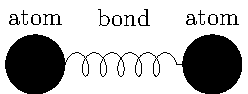
\includegraphics[width=0.25\linewidth]{atoms-spring.pdf}} \label{fig:qho-mod1}} \hspace{4ex}
	\subfloat[]{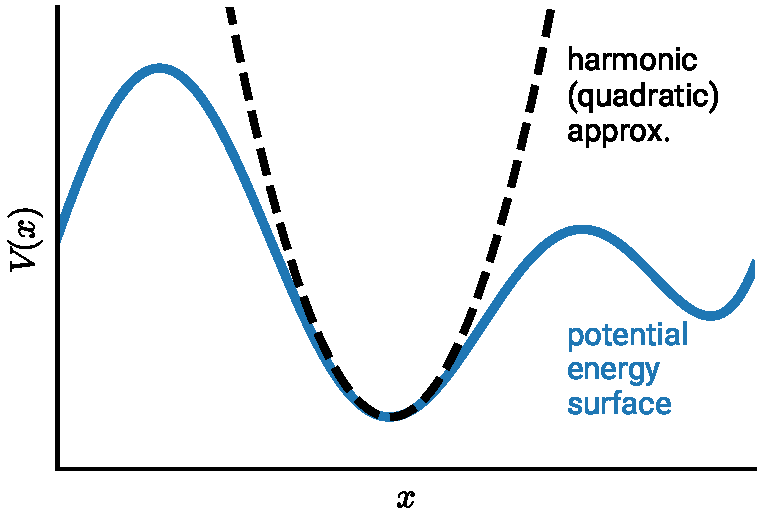
\includegraphics[width=0.43\linewidth]{qpot-min.pdf} \label{fig:qho-mod2}}
	\caption{The quantum harmonic oscillator is particularly powerful at modeling \protect\subref{fig:qho-mod1} the forces that hold atoms together, which are often approximated with springs, and 
	\protect\subref{fig:qho-mod2} the minima of any generic potential surface, which is approximately parabolic when one considers the Taylor series near the minimum.}
	\label{fig:qpot}
\end{figure}



% % % % % % % % % % % % % % % % % % % % % % % % % % % % % % % % % % % % % 
% % % % % % % % % % % % % % % % % % % % % % % % % % % % % % % % % % % % % 
% % % % % % % % % % % % % % % % % % % % % % % % % % % % % % % % % % % % % 
\section{Operators}

In order to work with the QHO, we will have to revisit the concept of \textbf{operators}, which are just special functions that represent physical observables. 
If we represent the quadratic potential energy in terms of angular frequency, i.e. $V(x) = \frac{1}{2} m\omega^2x^2$, we can then represent the Hamiltonian of the particle, which is the sum of the kinetic and potential energies, as

\begin{tcolorbox}[title = Hamiltonian for the QHO] \vspace{-2ex}
	\begin{equation}
	\hat{H} = \frac{\hat{p}^2}{2m} + \frac{1}{2}m\omega^2x^2 \label{eq:ham-qho}
	\end{equation}
\end{tcolorbox}

Notice that in the first term, we used $\hat{p}$ to represent the momentum operator, which is defined as $\hat{p} = -i\hbar\dv{x}$.\footnote{Technically position here is also an operator $\hat{x}$, but it \href{https://physics.stackexchange.com/questions/273272/derivation-of-position-operator-in-qm}{happens to be defined} as $\hat{x} = x$, so we leave off the hat.} 
Now we need to solve the time-independent \Sch\ equation, given by:

\begin{tcolorbox}[title = \Sch\ equation for the QHO] \vspace{-2ex}
	\begin{equation}
		\hat{H}\Psi = -\frac{\hbar^2}{2m}\dv[2]{\Psi}{x} + \frac{1}{2}m\omega^2x^2\Psi = E\Psi \label{eq:se-qho}
	\end{equation}
\end{tcolorbox}

Recall that this form for the operator $\hat{p}$ was motivated by the first wave equation we wrote down, corresponding to the free particle. 
This was an expression of the form $\exp\left(i(kx-\omega t)\right) = \exp \left( \frac{i}{\hbar}(px-Et) \right)$. 
If we act on this wave equation with the operator $\hat{p}$ defined as above, we get the same function back multiplied by $p$:

\begin{align*}
	\hat{p}\exp \left(\frac{i}{\hbar}(px-Et)\right) &= -i\hbar\exp \left(\frac{i}{\hbar}(px-Et)\right) \left(\frac{ip}{\hbar}\right) \\
	&= p\exp \left(\frac{i}{\hbar}(px-Et)\right)
\end{align*}

One can think of this as essentially representative of what it means to make a measurement of the momentum in a quantum mechanical system.



% % % % % % % % % % % % % % % % % % % % % % % % % % % % % % % % % % % % % 
% % % % % % % % % % % % % % % % % % % % % % % % % % % % % % % % % % % % % 
% % % % % % % % % % % % % % % % % % % % % % % % % % % % % % % % % % % % % 
\subsection{Ladder operators}

In order to solve \autoref{eq:se-qho}, we will attempt to \emph{factor} the Hamiltonian given by \autoref{eq:ham-qho}. 
To see the motivation behind this, notice that if the Hamiltonian was given by two real numbers $c^2 + d^2$, we could then factor this expression as 

\begin{equation*}
	c^2 + d^2 = (c + di)(c - di)
\end{equation*}

Following this example, we first reformulate the Hamiltonian so that we can factor it as follows:

\begin{align*}
	\hat{H} &= \frac{\hat{p}^2 }{2m} + \frac{1}{2}m\omega^2\hat{x}^2 \\
	&= \frac{m\omega^2}{2}\left[\hat{x}^2 + \frac{\hat{p}^2}{m^2\omega^2}\right] \\
	&= \frac{m\omega^2}{2}\left[\hat{x} + \frac{i\hat{p}}{m\omega}\right] \left[\hat{x}-\frac{i\hat{p}}{m\omega}\right] \numberthis \label{eq:ham-factored}
\end{align*}

\emph{A word of caution}: Though it may seem logical, we actually hand-waved a lot of the rigor here, because dealing with operators (which are functions) is trickier than dealing with real quantities (i.e., scalars). 
The theory is outside the scope of this course, but we will see shortly how this affects what are normally intuitive results. 

Now, the factored Hamiltonian in \autoref{eq:ham-factored} is suggestive of some form of symmetry, particularly the expressions inside the square brackets. 
We are now going to define two new operators:

\begin{tcolorbox}[title = Ladder operators] \vspace{-2ex}
	\begin{align}
		a &= \sqrt{\frac{m\omega}{2\hbar}}\left(\hat{x} + \frac{i\hat{p}}{m\omega}\right) = \sqrt{\frac{m\omega}{2\hbar}}\left(\hat{x} + \frac{\hbar}{m\omega}\dv{x}\right) \label{eq:annihile} \\
		\ad &= \sqrt{\frac{m\omega}{2\hbar}}\left(\hat{x} - \frac{i\hat{p}}{m\omega}\right) = \sqrt{\frac{m\omega}{2\hbar}}\left(\hat{x} - \frac{\hbar}{m\omega}\dv{x}\right) \label{eq:creation}
	\end{align}
\end{tcolorbox}

The method we are using to solve the \Sch\ equation in this chapter involves these two \textbf{ladder operators} $a$ and $\ad$ (read as: ``a-dagger"), which are known as the \textbf{annihilation}/\textbf{lowering} operator and \textbf{creation}/\textbf{raising} operator respectively (you will soon see why). 
This clever method was developed by Paul Dirac\footnote{Dirac was extremely influential in developing the formalism of quantum theory, introducing this and bra-ket notation which you will see later. He shared the 1933 Nobel Prize in Physics with \Sch. Curiously, Einstein describes that ``[he has] trouble with Dirac. This balancing on the dizzying path between genius and madness is awful.'' (N. Sukumar, \emph{A Matter of Density}, 2012).} and allows us to eventually solve for the energy without directly solving the \Sch\ equation. 
Note that we chose the coefficient of $\sqrt{m\omega/2\hbar}$ largely for the purpose of eliminating constants in the end.


% % % % % % % % % % % % % % % % % % % % % % % % % % % % % % % % % % % % % 
% % % % % % % % % % % % % % % % % % % % % % % % % % % % % % % % % % % % % 
% % % % % % % % % % % % % % % % % % % % % % % % % % % % % % % % % % % % % 
\subsection{Hamiltonian revisited}

We see that the ladder operators are individually defined in terms of the position and momentum operators, so why not try solving for them? 
If we add \autoref{eq:annihile} and \ref{eq:creation}, we get 

\begin{equation*}
	a + \ad = \sqrt{\frac{m\omega}{2\hbar}}2\hat{x}
\end{equation*}

\noindent which allows us to solve for the position operator as

\begin{tcolorbox}[title = Position operator] \vspace{-2ex}
	\begin{equation}
		\hat{x} = \sqrt{\frac{\hbar}{2m\omega}}\left(\ad + a \right) \label{eq:x-op}
	\end{equation}
\end{tcolorbox}

Similarly, we can subtract the two ladder operators to get

\begin{equation*}
	a - \ad = \sqrt{\frac{m\omega}{2\hbar}} \frac{2i\hat{p}}{m\omega}
\end{equation*}

\noindent which gives the momentum operator as 

\begin{tcolorbox}[title = Momentum operator] \vspace{-2ex}
	\begin{equation}
	\hat{p} = i\sqrt{\frac{m\omega\hbar}{2}}\left(\ad - a \right) \label{eq:p-op}
	\end{equation}
\end{tcolorbox}

OK, so why might this be useful? 
Let's rewrite the Hamiltonian in terms of these new operators:

\begin{align*}
	\hat{H} &= \frac{\hat{p}^2}{2m} + \frac{1}{2}m\omega^2\hat{x}^2 \\
	&= -\frac{1}{2m}\frac{m\omega\hbar}{2}\left(\ad - a\right)^2 + \frac{1}{2}m\omega^2 \frac{\hbar}{2m\omega} \left(\ad + a \right)^2 \\
	&= -\frac{\hbar\omega}{4} \left(\left(\ad\right)^2 - \ad a - a\ad + a^2\right) + \frac{\hbar\omega}{4}\left(\left(\ad\right)^2 + \ad a + a\ad + a^2 \right) \\
	\Aboxed{ \hat{H} &= \frac{\hbar\omega}{2} \left( \ad a + a\ad \right)} \numberthis \label{eq:ham-qho2}
\end{align*}

Now, we might be tempted to combine the $\ad a$ term with the $a \ad$ term, but this is one of the tricky aspects of operators: 
\textbf{In general, they do not commute} with each other, so we can't expect them to represent the same quantity when we switch the order. 

Of course, we shouldn't be fazed by this fact and we will try to see if we can find some relationship between the two terms. 
Luckily, in quantum mechanics, there is a quantity called the \textbf{commutator} (adopted from group theory) that precisely indicates to what degree two operators fail to commute. 
Given two operators $A$ and $B$, we define the commutator as

\begin{equation}
	[A,B] = AB - BA \label{eq:comm}
\end{equation}

\noindent which you can see for normal (scalar) variables should be zero.

As a first example, let's consider the commutation relation between $\hat{x}$ and $\hat{p}$, i.e. $[\hat{x}, \hat{p}]$. 
To aid the derivation, we will have both operators act on an arbitrary dummy function $\Psi$ that we will discard in the end.

\begin{align*}
	[\hat{x}, \hat{p}]\Psi &= (\hat{x}\hat{p})\Psi - (\hat{p}\hat{x})\Psi \\
	&= x\left(-i\hbar \dv{x}\Psi \right) + i\hbar \dv{x}(x\Psi) \\
	&= -i\hbar x \dv{x}\Psi + i\hbar x \dv{x}\Psi + i\hbar\Psi \\
	&= i\hbar\Psi 
\end{align*}

From this, one then concludes that 

\begin{tcolorbox}[title = Canonical commutation relation] \vspace{-2ex}
	\begin{equation}
		[\hat{x}, \hat{p}] = i\hbar
	\end{equation}
\end{tcolorbox}

\noindent which is known as the \textbf{canonical commutation relation} because it establishes a fundamental relationship between two conjugate variables, such as $\hat{x}$ and $\hat{p}$, that eventually leads to the uncertainty principle. 

Now what about the commutation relation between $a$ and $\ad$? 
The result actually follows nicely from the canonical commutation relation. 
First, we also show that if two operators can be expressed as $f+g$ and $f-g$, where $f$ and $g$ are arbitrary operators, then their commutation relation can be simplified as follows:

\begin{align*}
	[f+g,f-g] &= (f+g)(f-g) - (f-g)(f+g) \\
	&= f^2 - fg + gf -g^2 - f^2 - fg + gf + g^2 \\
	&= 2(gf - fg) \\
	&= 2[g,f]
\end{align*}

We can apply this result to find that

\begin{align*}
	[a, \ad] &= \frac{m\omega}{2\hbar}\left[\hat{x} + \frac{i\hat{p}}{m\omega}, \hat{x} - \frac{i\hat{p}}{m\omega} \right] \\
	&= \frac{m\omega}{\hbar} \left[ \frac{i\hat{p}}{m\omega}, \hat{x} \right] \\
	&= \frac{i}{\hbar}[\hat{p},\hat{x}] \\
	&= \frac{i}{\hbar}(-i\hbar) = 1
\end{align*}

\begin{tcolorbox}[title = Ladder operators commutation relation] \vspace{-2ex}
	\begin{equation}
		[a,\ad] = a\ad - \ad a = 1  \label{eq:a-comm}
	\end{equation}
\end{tcolorbox}


% % % % % % % % % % % % % % % % % % % % % % % % % % % % % % % % % % % % % 
% % % % % % % % % % % % % % % % % % % % % % % % % % % % % % % % % % % % % 
% % % % % % % % % % % % % % % % % % % % % % % % % % % % % % % % % % % % % 
\section{Solutions of the QHO}

We're almost there! 
Now using this commutation relation, we can rewrite \autoref{eq:ham-qho2} in its standard form. 
In particular, using the fact that $a\ad = 1 + \ad a$, we find that

\begin{tcolorbox}[title = Hamiltonian of the QHO (with ladder operators)] \vspace{-2ex}
	\begin{equation}
	\hat{H} = \hbar\omega \left(\ad a + \frac{1}{2} \right) \label{eq:ham-qho3}
	\end{equation}
\end{tcolorbox}

OK, now let's try to understand why all of the above definitions and mathematics are useful in terms of solving the QHO problem. 
To begin with, let's rewrite the time-independent \Sch\ equation in terms of these new variables. 
We have:

\begin{equation}
	\hbar\omega \left(\ad a + \frac{1}{2} \right)\psi_n = E_n\psi_n \label{eq:sch-qho}
\end{equation}

\noindent where we have introduced a quantum number $n$ as an index for the allowed solutions of this equation, just like we did for the particle in a box. 
Now let's act from the left on \autoref{eq:sch-qho} with the lowering operator $a$, carefully keeping track of the order of the operators since we know they don't commute with each other (but they can commute with scalars, like the energy $E_n$). 
This gives

\begin{align*}
	\hbar\omega \left(\ad a + \frac{1}{2} \right)\psi_n &= E_n\psi_n \\
	\hbar\omega \left(a \ad a + \frac{1}{2} a\right)\psi_n &= E_na\psi_n \\
	\hbar\omega \left(\left(1 + \ad a \right) a + \frac{1}{2} a\right)\psi_n &= E_na\psi_n \\
	\hbar\omega \left(1 + \ad a + \frac{1}{2} \right) a\psi_n &= E_na\psi_n \\
	\Aboxed{\hbar\omega \left(\ad a + \frac{1}{2} \right) (a\psi_n) &= (E_n-\hbar\omega)(a\psi_n)} \numberthis \label{eq:sch-qho2}
\end{align*}

If we look carefully at this equation and compare it to \autoref{eq:sch-qho}, we see that they are the same form! 
This says in particular that if $\psi_n$ is a solution of the QHO with energy $E_n$, then $a\psi_n$ is also a solution, with energy $E_n-\hbar\omega$. 
This is a key result and explains why $a$ is called the lowering operator. 
From a known solution one can essentially generate all other known solutions of lower energy by applying this operator. 
This is quite handy!

So imagine that one starts from some known solution and starts applying this operator, generating lower and lower energy states. 
At some point one must find the ground-state solution. 
But what happens if one then applies the lowering operator to this? 
If this gives some new function, then this can't really have been the ground state! 
We therefore conclude that the ground state wavefunction must satisfy the equation

\begin{equation*}
	a\psi_0 = 0
\end{equation*}

Here you can really see how we have successfully factorized the initial second order differential equation (\autoref{eq:se-qho}) to obtain a solution for the wavefunction. 
In particular, we can use the right hand side of \autoref{eq:annihile} to substitute for the lowering operator $a$ and obtain a first order differential equation:

\begin{equation*}
	\left(x + \frac{\hbar}{m\omega} \dv{x}\right)\psi_0 = 0
\end{equation*}

We can solve this using separation of variables as follows:

\begin{align*}
	\left(x + \frac{\hbar}{m\omega} \dv{x}\right)\psi_0 &= 0 \\
	\frac{\hbar}{m\omega} \dv{\psi_0}{x} &= -x\psi_0 \\
	\frac{1}{\psi_0} \dd{\psi_0} &= -\frac{m\omega}{\hbar}x \dd{x} \\
	\ln (\psi_0) &= -\frac{m\omega}{2\hbar}x^2 \\
	\Aboxed{\psi_0 &= A \exp \left(-\frac{m\omega}{2\hbar}x^2\right)} \numberthis
\end{align*}

We have to normalize the wavefunction the same way we always do, which allows us to solve for $A$ as

\begin{align*}
	\int_{-\infty}^{\infty} \abs{\psi_0}^2 \dd{x} &= 1 \\
	\abs{A}^2 \int_{-\infty}^{\infty} \exp \left(-\frac{m\omega}{\hbar} x^2 \right) \dd{x} &= 1 \\
	\abs{A}^2 \sqrt{\frac{\pi\hbar}{m\omega}} &= 1  \tag{We use $\displaystyle\int_{-\infty}^{\infty}e^{-ax^2} \dd{x} = \sqrt{\frac{\pi}{a}}$}\\
	\Aboxed{A &= \left(\frac{m\omega}{\pi\hbar}\right)^{1/4}} \numberthis
\end{align*}

Combining these two results finally gives us

\begin{tcolorbox}[title = Ground state for the QHO] \vspace{-2ex}
	\begin{equation}
		\psi_0 = \left(\frac{m\omega}{\pi\hbar}\right)^{1/4} \exp \left(-\frac{m\omega}{2\hbar}x^2\right) \label{eq:qho-ground}
	\end{equation}
\end{tcolorbox}

One can easily substitute this back into the \Sch\ equation to verify this indeed solves the differential equation---try it yourself! 
A sketch of this wavefunction has a Gaussian shape within the boundary of the potential with probability maximized at the center of the quadratic potential, analogous to the equilibrium position of the effective mass on a spring (\autoref{fig:qho-ground}). 
The key difference between this state and its classical analogue is that the quantum ground state has non-zero energy.

\begin{figure}[!h]
	\centering
	\includegraphics[width=0.38\linewidth]{qho-ground.pdf}
	\caption{A sketch of the ground state of the particle inside the parabolic potential. 
	The wavefunction has a Gaussian profile within the parabolic potential and it is centered about the minimum.}
	\label{fig:qho-ground}
\end{figure}


% % % % % % % % % % % % % % % % % % % % % % % % % % % % % % % % % % % % % 
% % % % % % % % % % % % % % % % % % % % % % % % % % % % % % % % % % % % % 
% % % % % % % % % % % % % % % % % % % % % % % % % % % % % % % % % % % % % 
\subsection{Zero-point energy}

What is the energy of the particle in this ground state? 
One can substitute \autoref{eq:qho-ground} into the differential equation and solve for $E_0$, or explicitly solve \autoref{eq:sch-qho} when $n = 0$. 
Both approaches work, and we will proceed with the latter approach to obtain

\begin{align*}
	\hbar\omega \left(\ad a + \frac{1}{2} \right)\psi_0 &= E_0\psi_0 \\
	\frac{\hbar\omega}{2}\psi_0 &= E_0\psi_0 \tag{since $a\psi_0=0$}
\end{align*}

\noindent which gives the energy for the ground state as

\begin{tcolorbox}[title = Zero-point energy] \vspace{-2ex}
	\begin{equation}
		E_0 = \frac{\hbar\omega}{2} \label{eq:zpe}
	\end{equation}
\end{tcolorbox}

This ground state energy is commonly referred to as \textbf{zero-point energy}, a concept that we've been alluding to previously. 
The zero-point energy arises due to quantum mechanical fluctuations between energy states that occur even at absolute zero, which explains, for example, why liquid helium does not freeze at standard pressure regardless of temperature.\footnote{Physicists Richard Feynman and John Wheeler have calculated that the zero-point energy in a vacuum the size of a light bulb is enough to boil all the world's oceans. See M. Pilkington, \href{https://www.theguardian.com/education/2003/jul/17/research.highereducation}{\emph{The Guardian}}, 2003.} 
Although it fits the context of the models presented in this course, the physical manifestations of zero-point energy are still poorly understood and are an active area of research.

Now we leave it as an exercise to the reader to show, using a similar procedure as above, that if $\psi_n$ is a solution with energy $E_n$, then $\ad\psi_n$ is also a solution with energy $E_n + \hbar\omega$ and thus $\ad$ behaves as a raising operator. 
Given this, we can now essentially reconstruct all solutions at least in principle by applying the raising operator to the known ground state solution. 
By this procedure, we can write down a clean result for the allowed energy states:

\begin{tcolorbox}[title = Allowed energy states of the QHO] \vspace{-2ex}
	\begin{equation}
		E_n = \hbar\omega\left(n + \frac{1}{2}\right) \label{eq:estates-qho}
	\end{equation}
\end{tcolorbox}

We see that like the particle in a box, the energy states of the QHO are quantized and indexed by the quantum number $n$. 
Where the two differ is that while the energy levels of the particle in a box scale as $n^2$, the energy levels here scale linearly in $n$, which means that these discrete energy levels are equally spaced by $\hbar\omega$. 

Now, you might be asking yourself if this procedure really generates all the possible solutions or just a subset of them. 
The answer is that it really does get them all! 
If there was some other state $\psi_m$ not generated by applying the raising operator successively from the ground state, one could lower this state by successively applying the lowering operator until eventually one arrives at the ground state satisfying $a\psi_0 = 0$. 
But this is just the ground state we've already uniquely identified and indicates that there are no other unique solutions of the \Sch\ equation that we've somehow missed.


% % % % % % % % % % % % % % % % % % % % % % % % % % % % % % % % % % % % % 
% % % % % % % % % % % % % % % % % % % % % % % % % % % % % % % % % % % % % 
% % % % % % % % % % % % % % % % % % % % % % % % % % % % % % % % % % % % %
\section{Additional properties}

\subsection{Bra-ket notation} \label{sec:braket}

We will start by formally introducing some notation to help us from here on out. 
Back in \autoref{ch:intro}, we used $\ket{S}$ as a way to describe quantum states. 
This is standard \textbf{bra-ket notation}, where $\ket{S}$ is called the \textbf{ket} and represents the state of the quantum system, whether it's the momentum, position, or something else. 
Every ket has an associated \emph{dual} or ``left half" called the \textbf{bra}, written as $\bra{S}$. 
Energy states can be expressed as $\ket{\Psi_0}$ or just $\ket{0}$ for short.

As you can probably imagine, the bra and ket can be combined together. 
Specifically, if we have $\bra{\Psi_m}$ and $\ket{\Psi_n}$ representing two quantum states, then this leads to

\begin{tcolorbox}[title = Bra-ket inner product] \vspace{-2ex}
	\begin{equation}
		\braket{\Psi_m}{\Psi_n} = 
		\int_{-\infty}^{\infty} \Psi_m^*\Psi_n \dd{x} \label{eq:bk-int}
	\end{equation}
\end{tcolorbox}

Essentially this notation is representing an \textbf{inner product}, which is a generalization of the dot product that you have seen in previous math classes. 
Indeed, one can think of a bra as a row vector that is multiplying a column vector ket. 
Furthermore, changing a quantum state from a bra to a ket (e.g. $\bra{f} \rightarrow \ket{f}$) is equivalent to taking the \textbf{conjugate transpose}. 
Working with this vector notation, we can also apply operators by multiplying them to the left of a ket, e.g.,

\begin{equation*}
	\hat{H} \ket{\Psi} = E\ket{\Psi} 
\end{equation*}

\noindent where you can treat $\hat{H}$ as an $n\times n$ matrix and $E$ as a constant.


% % % % % % % % % % % % % % % % % % % % % % % % % % % % % % % % % % % % % 
% % % % % % % % % % % % % % % % % % % % % % % % % % % % % % % % % % % % % 
% % % % % % % % % % % % % % % % % % % % % % % % % % % % % % % % % % % % %
\subsection{Expected value}

Since we work with probabilities in quantum mechanics, it is only suitable (and perhaps even delayed at this point) that we cover the concept of \textbf{expectation}, which can be thought of as the \textbf{average} or \textbf{mean} value. 
Given a quantity $x$, we denote the expected value of $x$ by $\expval{x}$. 
In general, the average value of some function of $x$ is given by 

\begin{equation}
	\expval{g(x)} = \sum_{i=1}^{\infty} g(x_i) p(x_i)
\end{equation}

\noindent where $p(x_i)$ is the probability of obtaining $g(x_i)$. 
This is the case for \emph{discrete} variables, such as the expected value of the roll of a die. 
For \emph{continuous} variables, we can't use a single probability for a point (it would be equal to zero), but rather a \textbf{probability density} $\rho(x)$ that can be applied over an interval. 
You're already experienced with probability densities since you've worked with the modulus squared of the wavefunction. 
Now our definition for the expectation of a function of a continuous variable becomes

\begin{equation}
	\expval{f(x)} = \int_{-\infty}^{\infty} f(x) \rho(x) \dd{x}
\end{equation}

When we're working with operators or physical observables, the expectations turn nicely into

\begin{equation}
	\expval{f(x)} = \int_{-\infty}^{\infty} \Psi^* f(x) \Psi \dd{x} = \mel{\Psi}{f}{\Psi} \label{eq:expval}
\end{equation}

Now, a measurement of the energy or momentum must return a real outcome, which means $\expval{f(x)}=\expval{f(x)}^*$. 
This can be rewritten as

\begin{equation*}
	\int_{-\infty}^{\infty} \Psi^* f(x) \Psi \dd{x} = \left( \int_{-\infty}^{\infty} \Psi^* f(x) \Psi \dd{x} \right)^* = \int_{-\infty}^{\infty} \left( f(x) \Psi\right)^* \Psi \dd{x}
\end{equation*}

\noindent or

\begin{equation}
	\braket{\Psi}{f\Psi} = \braket{f\Psi}{\Psi} \label{eq:hermitian}
\end{equation}

This condition defines the operator $f$ as \textbf{Hermitian}, which gives real values for the expectation and has real eigenvalues among its many nice properties. 
As a result, all quantum mechanical operators for physical observables are Hermitian, e.g., momentum, Hamiltonian, position, etc.


% % % % % % % % % % % % % % % % % % % % % % % % % % % % % % % % % % % % % 
% % % % % % % % % % % % % % % % % % % % % % % % % % % % % % % % % % % % % 
% % % % % % % % % % % % % % % % % % % % % % % % % % % % % % % % % % % % %
\subsection{Hermitian conjugates}

We show that $a$ and $\ad$ are \textbf{Hermitian conjugates} (or Hermitian adjoints), which are operators that are related by the following:

\begin{tcolorbox}[title = Hermitian conjugates] \vspace{-2ex}
	\begin{equation}
		\braket{f}{ag} = \braket{\ad f}{g} \label{eq:h-conj}
	\end{equation}
\end{tcolorbox}

\noindent for arbitrary $f$ and $g$. 
If we go back to the integral definition in \autoref{eq:bk-int}, we get that

\begin{equation*}
	\int_{-\infty}^{\infty} f^*ag \dd{x} = \int_{-\infty}^{\infty} (\ad f)^*g \dd{x}
\end{equation*}

\noindent which says that $a$ operating on $g$ must give the same result for the integral as $\ad$ operating on $f$. 
To prove this, we will use the differential form of the operator $a$ and integrate by parts.

\begin{align*}
	\braket{f}{ag} &= \int_{-\infty}^{\infty} f^* \left(x + \frac{\hbar}{m\omega} \dv{x} \right)g \dd{x} \\
	&= \int_{-\infty}^{\infty} f^*xg \dd{x} + \frac{\hbar}{m\omega} \int_{-\infty}^{\infty} f^* \dv{g}{x} \dd{x} \\
	&= \int_{-\infty}^{\infty} f^*xg \dd{x} + \frac{\hbar}{m\omega} \left[ \cancel{f^*g} \bigg|_{-\infty}^{\infty} - \int_{-\infty}^{\infty} \dv{f^*}{x} g \dd{x} \right] \tag{\href{https://tutorial.math.lamar.edu/classes/calcII/IntegrationByParts.aspx}{IBP!}} \\
	&= \int_{-\infty}^{\infty} \left[ \left(x - \frac{\hbar}{m\omega} \dv{x}\right) f \right]^* g \dd{x} \\
	&= \int_{-\infty}^{\infty} \left(\ad f\right)^*g \dd{x} \\
	&= \braket{\ad f}{g} 
\end{align*}

It is also true that

\begin{equation*}
	\braket{f}{\ad g} = \braket{af}{g}
\end{equation*}

We note here that even though the individual ladder operators are Hermitian conjugates, their \emph{product}, which appears in the Hamiltonian, \emph{is} a Hermitian operator.


% % % % % % % % % % % % % % % % % % % % % % % % % % % % % % % % % % % % % 
% % % % % % % % % % % % % % % % % % % % % % % % % % % % % % % % % % % % % 
% % % % % % % % % % % % % % % % % % % % % % % % % % % % % % % % % % % % %
\subsection{Scaling factor}

We already know that the raising and lowering operators generate new solutions of the \Sch\ equation. 
But this is defined only up to a proportionality factor. 
Given a normalized solution like $\psi_0$ found above, how do we find the higher order solutions exactly? 
We could normalize each one by brute force, but there is a nicer way. 
We start by saying that 

\begin{equation*}
	\ad \ket{\psi_n} = c_n \ket{\psi_{n+1}}
\end{equation*}

Next, we can apply the result of \autoref{eq:h-conj} in a clever way and note that

\begin{equation*}
	\braket{\ad \psi_n}{\ad \psi_n} = \braket{a\ad \psi_n}{\psi_n}
\end{equation*}

Then, if we take a closer look at our two expressions for the allowed energy states of the QHO (\autoref{eq:sch-qho} and \ref{eq:estates-qho}), we see that it must be the case that 

\begin{align}
	\ad a \psi_n &= n\psi_n \label{eq:ada-prop} \\
	a \ad \psi_n &= (\ad a + 1)\psi_n = (n+1)\psi_n \label{eq:aad-prop}
\end{align} 

We can combine these results to obtain

\begin{equation*}
	\braket{\ad \psi_n}{\ad \psi_n} = \braket{a\ad \psi_n}{\psi_n} = (n+1) \braket{\psi_n}{\psi_n} = \abs{c_n}^2\braket{\psi_{n+1}}{\psi_{n+1}}
\end{equation*}

Since $\psi_n$ and $\psi_{n+1}$ are normalized, it follows that $\abs{c_n}^2 = n+1$, and we have

\begin{tcolorbox}[title = Raising operator proportionality constant] \vspace{-2ex}
	\begin{equation}
		\ad \psi_n = \sqrt{n+1} \psi_{n+1} \label{eq:ad-prop}
	\end{equation}
\end{tcolorbox}

We will leave it as an exercise to the reader to derive (in essentially the same fashion) the proportionality coefficient for the lowering operator, which is 

\begin{equation}
	a \psi_n = \sqrt{n} \psi_{n-1} \label{eq:a-prop}
\end{equation}


% % % % % % % % % % % % % % % % % % % % % % % % % % % % % % % % % % % % % 
% % % % % % % % % % % % % % % % % % % % % % % % % % % % % % % % % % % % % 
% % % % % % % % % % % % % % % % % % % % % % % % % % % % % % % % % % % % %
\subsection{Orthogonality}
As you may have guessed by now, the stationary state solutions to the QHO are orthogonal,\footnote{In fact they also form an orthonormal basis.} which means that 

\begin{equation}
	\braket{\psi_m}{\psi_n} = \int_{-\infty}^{\infty} \psi_m^*\psi_n \dd{x} = \delta_{mn} \label{eq:ortho_qho}
\end{equation}

We can prove this using \autoref{eq:h-conj} and \ref{eq:ada-prop}. 
First, the second equation gives us

\begin{equation}
	\braket{\psi_m}{\ad a \psi_n} = \braket{\psi_m}{n\psi_n} = n\braket{\psi_m}{\psi_n} \label{eq:qho-orth1}
\end{equation}

However, we can also apply the first equation twice to the left hand side and obtain

\begin{equation}
	\braket{\psi_m}{\ad a \psi_n} = \braket{a \psi_m}{a \psi_n} = \braket{\ad a \psi_m}{\psi_n} = m\braket{\psi_m}{\psi_n} \label{eq:qho-orth2}
\end{equation}

Putting \autoref{eq:qho-orth1} and \ref{eq:qho-orth2} together, one obtains

\begin{equation*}
	(m-n)\braket{\psi_m}{\psi_n} = 0
\end{equation*}

\noindent which shows that if $m \neq n$, then 

\begin{equation*}
	\braket{\psi_m}{\psi_n} = \int_{-\infty}^{\infty} \psi_m^*\psi_n \dd{x} = 0
\end{equation*}

\noindent and the orthogonality condition is satisfied. 


% % % % % % % % % % % % % % % % % % % % % % % % % % % % % % % % % % % % % 
% % % % % % % % % % % % % % % % % % % % % % % % % % % % % % % % % % % % % 
% % % % % % % % % % % % % % % % % % % % % % % % % % % % % % % % % % % % %
\section[Applications]{Applications of the QHO}

By now we've seen just how powerful the QHO model is and how useful some of these properties are. 
The existence of an exact, analytical solution to the QHO makes it a powerful framework for developing more advanced theories to analyze complex quantum mechanical systems. 
We mentioned at the beginning of this chapter how the QHO could be used to model subatomic particles and the forces between atoms, but a proper treatment involves delving a little deeper into \textbf{quantum field theory} (QFT), which is a framework that is partially derived from the concepts presented in this chapter. 
Rather than cramming this rich topic into a section here, we will instead be devoting the entire next chapter to QFT and combining the results from QFT and the QHO to analyze vibrational modes in solids called \textbf{phonons}. 
Stay tuned!

For the time being, however, let's briefly revisit the wavefunction solutions we derived earlier. 
We sidestepped a lot of the ugly algebra by employing the ladder operators method, but I would be doing you a disservice (particularly if you continue to study quantum mechanics in a different field like physics or electrical engineering), if I didn't at least mention the analytic method using \textbf{power series}.\footnote{We will skip all the details here, but there's a thorough derivation in Griffiths, Chapter 2.3.} 
When we work out the math, we arrive at the following expression for the stationary states of the QHO:\footnote{I encourage you to derive another expression for the $n^{\text{th}}$ stationary state using just the ladder operators! \emph{Hint}: The expression is far more concise, albeit recursive.} 

\begin{equation}
	\psi_n(x) = \left(\frac{m\omega}{\pi\hbar}\right)^{1/4} \frac{1}{\sqrt{2^n \cdot n!}} H_n \left(\sqrt{\frac{m\omega}{\hbar}}x\right) \exp \left(-\frac{m\omega x^2}{2\hbar}\right) \label{eq:pow-qho}
\end{equation}

\noindent where $H_n$ are the \textbf{Hermite polynomials}, given explicitly and recursively by

\begin{align*}
	H_n(z) &= (-1)^n e^{z^2} \dv[n]{z} \left( e^{-z^2} \right) \tag{explicit def.} \\
	H_n(z) &= 2zH_{n-1}(z) - 2(n-1)H_{n-2}(z) \tag{recursive def.}
\end{align*}

More concretely, the first few Hermite polynomials are

\begin{align*}
	H_0(z) &= 1 \\
	H_1(z) &= 2z \\
	H_2(z) &= 4z^2-2 \\
	H_3(z) &= 8z^3 - 12z \\
	H_4(z) &= 16z^4 - 48z^2 + 12
\end{align*}

The benefit of this method is that we have a closed-form expression for the wavefunction at any energy level. 
We already saw what the ground state $\psi_0$ looked like, which had maximum amplitude at the center of the quadratic potential, so now we plot $\abs{\psi_{50}}$ in \autoref{fig:qho-50}.

\begin{figure}[!h]
	\centering
	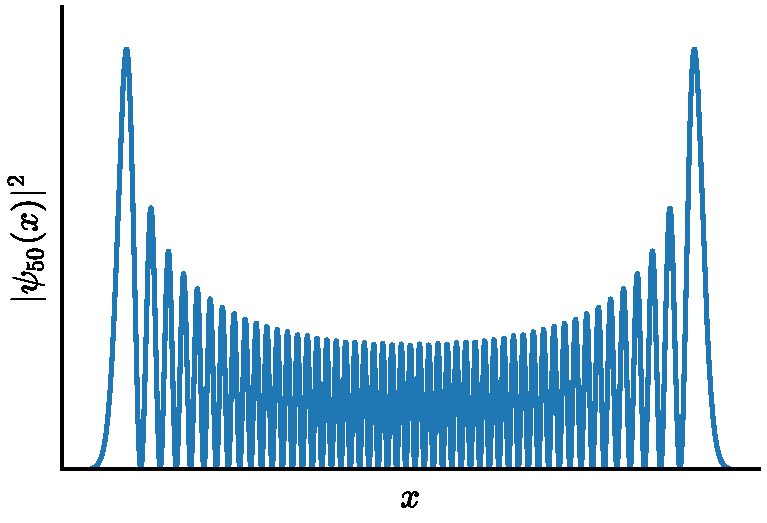
\includegraphics[width=0.5\linewidth]{hermite.pdf}
	\caption{The probability density function of the QHO with $n = 50$ contains nodes where the probability of finding the particle is zero. 
	The general profile also resembles the probability density of a classical harmonic oscillator.}
	\label{fig:qho-50}
\end{figure}

There are two interesting properties of this probability density function. 
First, notice that there are nodes where the probability of finding the particle is zero, just like the particle in a box. 
This is true of all energy states above the ground state. 
Second, we notice that the profile looks very different from the ground state; namely, the regions of largest probability are at the sides instead of the middle. 
This actually corresponds to a classical harmonic oscillator if you think about it---a moving mass on a spring with high elastic potential energy will spend the longest amount of time when it's most stretched out or most compressed (it moves the slowest as it changes direction), whereas it will move the fastest when it passes the equilibrium position (so the probability of finding it there is low, assuming it vibrates continuously without loss). 
Thus we see a nice analogy where the high-energy quantum mechanical system begins to exhibit classical behavior.


% % % % % % % % % % % % % % % % % % % % % % % % % % % % % % % % % % % % % 
% % % % % % % % % % % % % % % % % % % % % % % % % % % % % % % % % % % % % 
% % % % % % % % % % % % % % % % % % % % % % % % % % % % % % % % % % % % %
\section{Summary}

Whew! This was a lengthy chapter that was heavy on operators and bra-ket notation. 
Using ladder operators, we derived the ground state of the quantum harmonic oscillator, from which one can theoretically construct all the stationary states. 
We also discovered zero-point energy and determined that the allowed energies of the QHO are evenly spaced by $\hbar\omega$. 
I hope you found the derivations conducive towards your learning, and please come talk to me in office hours if something is unclear! 
Students find it helpful to try deriving some of these equations on their own to ensure full understanding. 
In the next chapter we will explore quantum field theory as an extension of the concepts presented here.

%} % for doublespacing
%\end{document}	% Quantum harmonic oscillators

% Created: Enze Chen, August 2017
% Updated: Aaron Lindenberg, 2018
% Last edited: Enze Chen, February 2018
%
% Chapter 7 of the MSE 142 coursereader.

% Uncomment the following three lines and last line to individually compile this chapter
%\documentclass[12pt, english]{book}
%\usepackage{142crstyle}
%\begin{document}

\chapter{Quantum Field Theory} \label{ch:qft}
%{ \doublespacing 
One of the greatest challenges facing scientists of the 20th century was using quantum mechanics to accurately model the behavior of subatomic particles, which usually involved painstakingly reconciling quantum mechanics with special relativity. Eventually, they developed the framework of quantum field theory (QFT), which treats particles as excited states (quanta) of the underlying \emph{field} (hence the name).\footnote{For an interesting explanation with helpful diagrams, see \href{https://www.ribbonfarm.com/2015/08/20/qft/}{this post} from Brian Skinner.} We can think of a field as a network of interconnected balls and springs and the strength of the field can be measured by the amount of displacement from rest. In this chapter, we will only scratch the surface of QFT as we explore some of its most surprising and most important results. \par 

\section{Second quantization}
So far, all of the systems we have analyzed fall into the category of \textbf{first quantization}, where we describe a quantum mechanical system by its wavefunction and we describe its surroundings (e.g. the potential well) using classical mechanics. While this formulation is well-defined for a single-particle system, many of its expressions grow combinatorially unwieldy for many-particle systems. In QFT, we are less concerned with the behavior of individual particles (``Which state is particle $i$ in?'') and we're more interested in the overall distribution (``How many particles are in state $\alpha$?''). This calls for \textbf{second quantization}, which places a QHO at each point in space such that the strength of the field is quantized. \par 

\subsection{Occupation number operator}
Recall that for single particles, we used bra-ket notation to represent the quantum state as $\ket{\alpha}$, where $\alpha = 0,\ 1,\ 2,\ \dots$. Now we will define the \textbf{occupation number operator} $\hat{n}_{\alpha}$ to be the number of particles in the single-particle state $\ket{\alpha}$. These occupation numbers label the basis state, which is represented as

\begin{tcolorbox} [title=Basis vector] \vspace{-2ex}
	\begin{equation}
		\ket{\Psi} = \ket{\hat{n}_0,\ \hat{n}_1,\ \hat{n}_2,\ \dots,\ \hat{n}_{\alpha},\ \dots} \label{eq:fock}
	\end{equation}
\end{tcolorbox} 

For bosons, $\hat{n}_{\alpha}$ can be any non-negative integer, while for fermions $\hat{n}_{\alpha}$ must be 0 or 1.\footnote{Bosons are a class of subatomic particles that have integer spins (e.g. photons, gluons, and other force carriers), while fermions are another class of subatomic particles that have non-integer spins (e.g. electrons) and obey the Pauli exclusion principle.} This formalism allows us to treat the quantum system as an ensemble of indistinguishable particles. The total number of particles is then
\begin{equation}
	\hat{N} = \sum_{\alpha} \hat{n}_{\alpha}
\end{equation}
which sums all the particles in all the states. \par 

To get a better understanding of the basis vectors, let's consider some special cases. First, there is a \textbf{vacuum state} with no particles represented as
\begin{equation}
	\ket{0} = \ket{0,\ 0,\ 0,\ \dots}
\end{equation}

The single-particle state that we've previously encountered can be written as
\begin{equation}
	\ket{1_{\alpha}} = \ket{0,\ 0,\ \dots, 1_{\alpha},\ \dots} = \psi_{\alpha}
\end{equation}

From this point, many-particle, many-state bases can be easily deduced, and we'll leave it as an exercise to the reader to find the proper normalization coefficient. \par 

Noticeably, the basis vector we defined in Equation~\ref{eq:fock} does not have a fixed particle number. This allows us to introduce and take away particles from our quantum mechanical system, which is conveniently handled by the creation and annihilation operators. \par 

\subsection{Creation and annihilation operators}

In the previous chapter, we used the creation and annihilation operators to arrive at different energy states of the quantum harmonic oscillator. Here, since we are dealing with an ensemble of many particles in many states, we will have a different $\ad_{\alpha}$ and $a_{\alpha}$ for each state $\ket{\alpha}$. Furthermore, the definition of the operators has changed, and now the creation operator acts as if it's truly ``creating'' another particle and adding it to the system. Formally, we have
\begin{equation}
	\ad_{\alpha} \ket{\hat{n}_1,\ \hat{n}_2,\ \dots,\ \hat{n}_{\alpha},\ \dots} = \sqrt{\hat{n}_{\alpha}+1}\ket{\hat{n}_1,\ \hat{n}_2,\ \dots,\ \hat{n}_{\alpha}+1,\ \dots}
\end{equation} 

Similarly, we define the annihilation operator as
\begin{equation}
a_{\alpha} \ket{\hat{n}_1,\ \hat{n}_2,\ \dots,\ \hat{n}_{\alpha},\ \dots} = \sqrt{\hat{n}_{\alpha}}\ket{\hat{n}_1,\ \hat{n}_2,\ \dots,\ \hat{n}_{\alpha}-1,\ \dots}
\end{equation} 

A simple demonstration of the creation operator would be to apply it to the vacuum state to obtain the single-particle state
\begin{equation}
	\ad_{\alpha} \ket{0} = \ket{1_{\alpha}}
\end{equation}

Likewise, if we apply the annihilation operator to the vacuum state, or any basis vector with zero particles in the particular state, we get zero.
\begin{equation}
	a_{\alpha} \ket{0} = 0, \qquad a_{\alpha} \ket{\hat{n}_1,\ \dots,\ \hat{n}_{\alpha}=0,\ \hat{n}_{\beta},\ \dots} = 0
\end{equation}

If we apply the annihilation operator and creation operator in succession, we obtain
\begin{equation*}
\ad_{\alpha} a_{\alpha} \ket{\hat{n}_1,\ \hat{n}_2,\ \dots,\ \hat{n}_{\alpha},\ \dots} = \hat{n}_{\alpha}\ket{\hat{n}_1,\ \hat{n}_2,\ \dots,\ \hat{n}_{\alpha},\ \dots}
\end{equation*}

which gives the relation
\begin{equation}
	\hat{n}_{\alpha} = \ad_{\alpha}a_{\alpha}
\end{equation}


This is similar to what we saw with the QHO and is another definition for the number operator. We will also state the commutation relations here without proof. Note that these are the same commutation relations as the QHO, and it's perfectly valid in QFT to consider bosons as energy quanta of an underlying field of quantum oscillators.
\begin{equation}
	\left[\ad_{\alpha},\ad_{\beta}\right] = \left[a_{\alpha},a_{\beta}\right] = 0, \qquad \left[a_{\alpha}, \ad_{\beta}\right] = \delta_{\alpha,\beta}
\end{equation}

With the formal definitions of second quantization out of the way, we can proceed to a more interesting analysis. Since we have an operator that gives the number of particles of each state in our system, we can find the total energy of all the particles by a simple sum. The expression for the Hamiltonian becomes
\begin{equation}
	\hat{H} = \sum_{\alpha} \hbar\omega_{\alpha} \left(\hat{n}_{\alpha} + \frac{1}{2} \right) = \sum_{\alpha} \hbar\omega_{\alpha} \left(\ad_{\alpha}a_{\alpha} + \frac{1}{2}\right)
\end{equation}


Here we give each quantum state its individual frequency $\omega_{\alpha}$. Now, as we showed in the last chapter, the Hamiltonian is a Hermitian operator, which means it should return a sensible value for the expectation. If we find the expected total energy of the vacuum state, we get the following:
\begin{align*}
	\mel{0}{\hat{H}}{0} &= \sum_{\alpha} \hbar\omega_{\alpha} \cancelto{0}{\mel{0}{\ad_{\alpha}a_{\alpha}}{0}} + \sum_{\alpha}\hbar\omega_{\alpha}\left(\frac{1}{2}\right) \\
	&= \sum_{\alpha} \frac{\hbar\omega_{\alpha}}{2} \rightarrow \infty
\end{align*}

In the second line, the summation of zero-point energies over an unbounded number of possible states seemingly gives infinite energy from vacuum fluctuations alone. Crazy! One of the early results of QFT was that the underlying field is in constant flux and it has physically relevant consequences. We'll see in the next section how we might resolve this ``infinite energy'' to make it physically interpretable.


%%%%%%%%%%%%%%%%%%%%%%%%%%%%%%%%%%%%%%%%%%%%%%%%%%%%%%%%%%%%%%%%%%%%%%%%%%%%%%%%

\section{Quantum electrodynamics}
One of the crowning achievements of QFT is the construction of \textbf{quantum electrodynamics} (QED), which describes how light and matter interact in the quantized electromagnetic field.\footnote{For a great introduction to QED in layman terms, see R. P. Feynman, \href{https://en.wikipedia.org/wiki/QED:_The_Strange_Theory_of_Light_and_Matter}{\emph{QED: The Strange Theory of Light and Matter}}. 1st ed., Princeton, NJ, Princeton University Press, 1985.} QED was the first theory to reconcile quantum mechanics and special relativity, and it led to extremely accurate calculations for the Lamb shift,\footnote{A good description of the Lamb shift is provided by \href{http://hyperphysics.phy-astr.gsu.edu/hbase/quantum/lamb.html}{Rod Nave}.} spontaneous emission (discussed in the next chapter), and a mysterious phenomenon called the Casimir effect, which we will discuss here. As it turns out, all of these phenomenon can be easily explained by the vacuum fluctuation energy and the way it interacts with matter.

%\subsection{Renormalization}

\begin{figure}[!h]
	\centering
	\subfloat[]{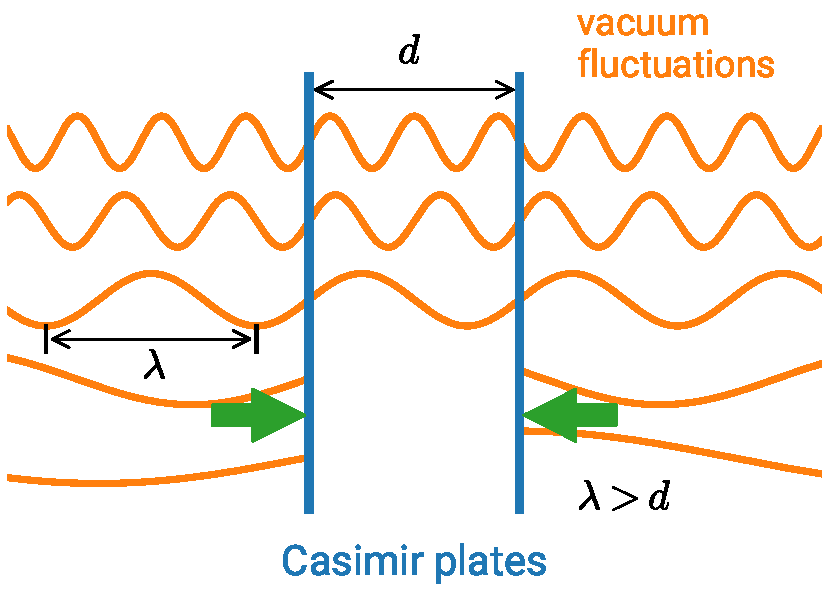
\includegraphics[width=0.5\linewidth]{casimir} \label{casimir-fig}} \hspace{2ex}
	\subfloat[]{\includegraphics[width=0.45\linewidth]{casimir-exp} \label{casimir-exp}}
	\caption{\protect\subref{casimir-fig} A schematic of the Casimir effect observed between two metal plates. The boundary conditions at the plates allow a limited number of standing waves to exist in the middle region, which is fewer than the amount of vacuum fluctuations outside the plates. This creates a pressure difference that forces the plates together. \protect\subref{casimir-exp} An experimental measurement using an atomic force microscope of the Casimir force between an Al-coated sphere and an Al-coated surface. Reproduced from U. Mohideen and A. Roy, \href{https://journals.aps.org/prl/abstract/10.1103/PhysRevLett.81.4549}{\emph{Phys. Rev. Lett.}} \textbf{81}, 4549 (1998).}
	\label{fig:casimir}
\end{figure}

\subsection{Casimir effect}
In 1948, Dutch physicist Hendrik Casimir predicted that the zero-point energy in the QED vacuum could cause a physical force between two neutral conducting plates.\footnote{H. B. G. Casimir, \href{http://www.dwc.knaw.nl/DL/publications/PU00018547.pdf}{\emph{Proc. Kon. Ned. Akad. Wetensch.}} \textbf{51}, 793 (1948)} This phenomenon became known as the \textbf{Casimir effect} (Figure~\ref{fig:casimir}) and can be explained using QED and second quantization. Although there are infinite vacuum fluctuations in the space outside of the plates, the reflective surface of the plates actually exclude virtual photons (manifestations of the underlying field) with wavelengths longer than the interplanar distance. Essentially you can think of the plates as nodes for the wave-like photons, so only wavelengths that line up perfectly will remain in the middle region. This reduces the energy density between the two plates, and much like normal pressure, the Casimir force pushes the two plates closer together. \par 

Since we should not be merely satisfied with a description, let's try to find an analytical argument and really derive the strength of this Casimir force. Since we are working with the QED vacuum, we have to first establish the \textbf{dispersion relation} for photons, which gives the relationship between the frequency and the wave number. Mathematically, this is written as
\begin{tcolorbox}[title=Dispersion relation] \vspace{-2ex}
	\begin{equation}
		\omega_n = ck_n \label{eq:dispersion}
	\end{equation}
\end{tcolorbox}

where $c$ is the speed of light and $k_n = n\pi/d$. We also make use of the subscript $n$ here to index individual solutions, just like we did with the particle in a box. \par 

\subsection{Regularization and renormalization}

Now we will try to find the amount of energy in between the two plates and subtract that quantity from the energy on the outside, and that should give us quantitative information about the Casimir force (its derivative will, anyways). Inside the two conducting plates, we have the following expression for the total energy:
\begin{align*}
	E_{\text{in}} &= \sum_{\alpha} \frac{\hbar\omega_{\alpha}}{2} \\
	&= \sum_{n=0}^{\infty} \frac{\hbar c k_n}{2} \\
	&= \frac{\hbar \pi c}{2d} \sum_{n=1}^{\infty} n \numberthis \label{eq:casimir-in}
\end{align*}

We use a discrete sum for the discrete energy levels of the bound photons, and just like before, we see that the total energy approaches infinity. Now, those of you that have taken complex analysis might see the summation and realize where this is headed---and yes indeed, it is possible to use analytical methods such as \textbf{zeta function regularization} to evaluate the sum of natural numbers by assigning a finite value to an otherwise divergent sum.\footnote{See \href{https://en.wikipedia.org/wiki/1_\%2B_2_\%2B_3_\%2B_4_\%2B_\%E2\%8B\%AF}{Wikipedia} for an interesting discussion about $1+2+3+4+\cdots$.}
\begin{equation}
	 \sum_{n=1}^{\infty} n = 1 + 2 + 3 + 4 + \cdots = -\frac{1}{12}   \label{eq:sumN}
\end{equation}

We will come back to this shortly, and as bizarre as this is, I ask you to trust me for the time being. We still have to find the total energy of the virtual photons \emph{outside} of the metal plates, which is similar to Equation~\ref{eq:casimir-in}, except we will now take an integral (instead of a sum) because the modes are no longer confined to be integers and can be any non-negative real number. Proceeding, we have
\begin{align*}
	E_{\text{out}} &= \frac{\hbar \pi c}{2d} \int_0^{\infty} n \dd{n} \\
	&= \frac{\hbar \pi c}{2d} \lim\limits_{s \rightarrow 0} \int_0^{\infty} ne^{-sn} \dd{n} \\
	&= \frac{\hbar \pi c}{2d} \lim\limits_{s \rightarrow 0} \int_0^{\infty} \dv{s} \int ne^{-sn} \dd{s} \dd{n} \\
	&= -\frac{\hbar \pi c}{2d} \lim\limits_{s \rightarrow 0} \dv{s} \int_0^{\infty} e^{-sn} \dd{n} \\
	&= -\frac{\hbar \pi c}{2d} \lim\limits_{s \rightarrow 0} \dv{s} \left(-\frac{1}{s} e^{-sn} \bigg|_0^{\infty} \right) \\
	&= -\frac{\hbar \pi c}{2d} \lim\limits_{s \rightarrow 0} \dv{s} \left( \frac{1}{s} \right) \\
	E_{\text{out}} &= \frac{\hbar \pi c}{2d} \lim\limits_{s \rightarrow 0} \frac{1}{s^2} \numberthis \label{eq:casimir-out} 
\end{align*}

In going from the first line to the second, we employed \textbf{exponential regularization} to transform the integrand into something more manageable. Regularization is a common trick in QFT for dealing with infinities by employing a ``cutoff'' function to model physics at unobserved length scales. You can check for yourself that by taking the limit as $s$ approaches 0 we get back our original integral. In the third line we insert a derivative and integral with respect to $s$ to cleverly simplify our expression. These are \emph{not} obvious steps, so don't worry if you find yourself asking how you would know to do this on your own. I wish to simply expose you to this technique, and as long as you are able to follow along, it is sufficient for this course. \par 

Of course, the question we \emph{should} be asking is how we could possibly subtract the two expressions we obtained in Equation~\ref{eq:casimir-in} and~\ref{eq:casimir-out}, which both approach infinity, and still get a non-zero result. As you may recall from calculus, some infinities are bigger than other infinities,\footnote{\href{https://en.wikipedia.org/wiki/Cantor\%27s_diagonal_argument}{Cantor's diagonal argument} is one proof of this fact, and \href{https://www.khanacademy.org/math/math-for-fun-and-glory/vi-hart/infinity/v/proof-infinities}{Vi Hart} gives a great explanation in their video.
See also \href{https://www.scientificamerican.com/article/a-deep-math-dive-into-why-some-infinities-are-bigger-than-others/}{this SciAm article}.} so as long as we can quantify \emph{how much} greater one expression is than the other, then we can reach a finite result. This touches upon the concept of \textbf{renormalization}, which is the other technique physicists use to handle infinities in QFT by assigning physical quantities to match observed values, thereby correcting for length-scale differences and self-interaction effects. \par 

Just as we did in the derivation for $E_{\text{out}}$, we will also apply regularization to the expression we obtained for $E_{\text{in}}$. We will move quickly through the derivations here, and leave the details for Appendix~\ref{sec:casimir-deriv}. Proceeding, we have:
\begin{align*}
	E_{\text{in}} &= \frac{\hbar \pi c}{2d} \sum_{n=1}^{\infty} n \\
	&= \frac{\hbar \pi c}{2d} \left( - \lim\limits_{s \rightarrow 0} \dv{s} \sum_{n=0}^{\infty} e^{-sn} \right) \\
	&= \frac{\hbar \pi c}{2d} \left( - \lim\limits_{s \rightarrow 0} \dv{s} \frac{1}{1-e^{-s}} \right)
\end{align*}

where we have used the sum of an infinite geometric series with common ratio $e^{-s}$ to arrive at the last line. Now we can evaluate the derivative to obtain
\begin{equation*}
	E_{\text{in}} = \frac{\hbar \pi c}{2d} \left( \lim\limits_{s \rightarrow 0} \frac{e^{s}}{(e^s-1)^2} \right)
\end{equation*}

Now if we rewrite the last line using the Taylor series expansion around $s=0$, we get
\begin{align*}
	E_{\text{in}} &= \frac{\hbar \pi c}{2d} \lim\limits_{s \rightarrow 0} \left( \frac{1+s+s^2/2 + \cdots}{(s + s^2/2 + s^3/6 + \cdots)^2} \right) \\
	&= \frac{\hbar \pi c}{2d} \lim\limits_{s \rightarrow 0} \left( \frac{1}{s^2} - \frac{1}{12} + \mathcal{O}(s^2) \right) \numberthis \label{eq:casimir-in2}
\end{align*}

As $s$ approaches 0, we can discard the terms of order 2 and greater, and subtract Equation~\ref{eq:casimir-in2} from Equation~\ref{eq:casimir-out}. This leaves us with 
\begin{equation*}
	E_{\text{out}} - E_{\text{in}} = \frac{\hbar \pi c}{2d} \left[ \frac{1}{s^2} - \left( \frac{1}{s^2} - \frac{1}{12} \right) \right] = \frac{\hbar \pi c}{24d}
\end{equation*}

\begin{tcolorbox}[title=Casimir force in one dimension] \vspace{-2ex}
	\begin{equation}
		F_{\text{cas}} = -\dv{E}{d} = -\frac{\hbar \pi c}{24d^2}
	\end{equation}
\end{tcolorbox}

In three dimensions, the Casimir force per unit area (a ``pressure'' quantity) becomes 
\begin{equation*}
	\frac{F_{\text{cas}}}{A} = -\frac{\hbar\pi^2c}{240d^4}
\end{equation*}

The negative sign here signifies an attractive force, which is what we expect if the energy density is larger on the outside of the plates than on the inside. The presence of $\hbar$ also means $F_{\text{cas}}$ is very small and hence only observable on the nanoscale. \par 

The Casimir effect was finally measured experimentally by Steven K. Lamoreaux in 1997,\footnote{S. K. Lamoreaux, \href{https://journals.aps.org/prl/abstract/10.1103/PhysRevLett.78.5}{\emph{Phys. Rev. Lett.}} \textbf{78}, 5 (1997).} and the photo in Figure~\ref{fig:casimir} is another experimental setup by Umar Mohideen that achieved measurement accuracy within 1\% of the theoretical value. The Casimir force significantly dominates the other fundamental forces at nanometer length scales and plays an important role in the performance of nanoelectronics and nanodevices. What's perhaps most surprising about the Casimir effect is that the force can change between attractive and repulsive simply based on the geometry of the conducting plates! \par

%%%%%%%%%%%%%%%%%%%%%%%%%%%%%%%%%%%%%%%%%%%%%%%%%%%%%%%%%%%%%%%%%%%%%%%%%%%%%%%%

\section{Application: Phonons}
Materials scientists typically work with condensed matter (solids and liquids) whose atom centers are analogous to the arrangement of harmonic oscillators in the quantum field. The periodicity of the atom centers in a crystal, much like what we saw in Chapter~\ref{ch:period}, leads to distinct vibrational modes that are quantized as \textbf{phonons} (Figure~\ref{fig:phonons}). Nearest neighbor interactions (electrostatic forces, van der Waals forces, etc) create an energy landscape that is well approximated by a parabolic potential surface, much like the QHO. Analyzed in the framework of second quantization, phonons behave exactly like bosons, with the same Hamiltonian, creation and annihilation operators, and commutation relations. 

\begin{figure}[!h]
	\centering
	\includegraphics[width=0.5\linewidth]{phonons}
	\caption{Collective vibrations in a crystal are quantized as phonons.}
	\label{fig:phonons}
\end{figure}

Phonons play a major role in the electrical conductivity, thermal conductivity, and thermal capacity of condensed matter. One of the most interesting features of phonons is when there are two different atoms vibrating next to each other, which results in two different phonon modes. The dispersion relation is given by the following equation and it is plotted in Figure~\ref{fig:phonon-modes}.
\begin{equation}
	\omega^2 = \frac{C}{m_1m_2} \left(m_1 + m_2 \pm \sqrt{m_1^2 + m_2^2 + 2m_1m_2\cos(kd)}\right)
\end{equation}

\begin{figure}[!h]
	\centering
	\subfloat[]{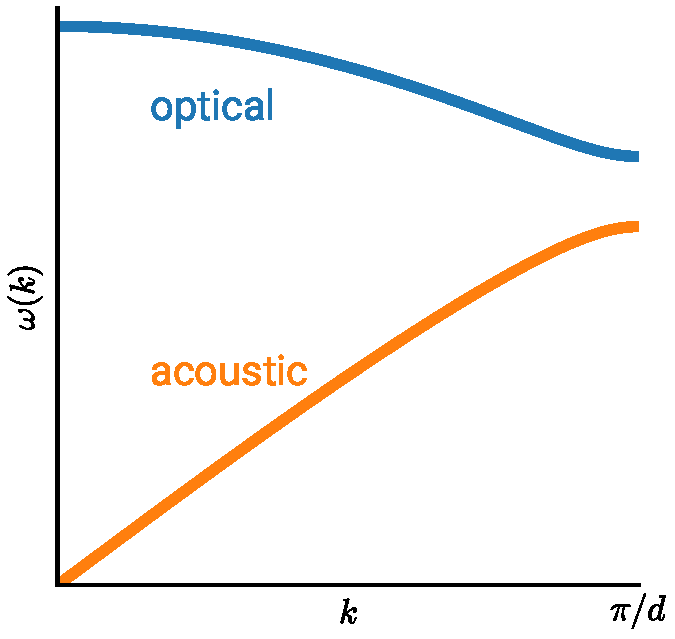
\includegraphics[width=0.5\linewidth]{phonon-modes} \label{phonon-modes}} \hspace{3ex}
	\subfloat[]{\includegraphics[width=0.37\linewidth]{phonon-absorption} \label{phonon-absorption}}
	\caption{\protect\subref{phonon-modes} Dispersion relation for phonons in a solid with two atoms per unit cell. The acoustic mode governs thermomechanical properties while the optical mode governs electronic properties. \protect\subref{phonon-absorption} Transmissivity of a film of RbI at different temperatures, with each minimum at a photon energy equal to that of the long wavelength transverse optical phonon. Reproduced from G. O. Jones \emph{et al.} \href{http://rspa.royalsocietypublishing.org/content/261/1304/10}{\emph{Proc. R. Soc. Lond.}} \textbf{A261}, 10-27, (1961).}
	\label{fig:phonon-modes}
\end{figure}

When atoms are vibrating coherently (in the same direction; corresponding to the minus sign in the above equation), \textbf{acoustic phonons} are produced, named because they regulate the speed of sound in the medium as well as the medium's mechanical and thermal properties.\footnote{See A. A. Balandin \href{https://www.nature.com/nmat/journal/v10/n8/full/nmat3064.html}{\emph{Nature Materials}}, \textbf{10}, 569-581 (2011) for a review of the thermal properties of carbon nanostructures.} On the other hand, atoms vibrating out-of-phase (in opposite directions) will produce \textbf{optical phonons}, which interact with light in absorption and \emph{Raman scattering}. 

%%%%%%%%%%%%%%%%%%%%%%%%%%%%%%%%%%%%%%%%%%%%%%%%%%%%%%%%%%%%%%%%%%%%%%%%%%%%%%%%

\section{Summary}
To recap, this chapter gave us a taste of quantum field theory and some of its important applications. Second quantization provided a suitable framework for interpreting fields with the new occupation number operator and new definitions for the creation and annihilation operators. Then we explored the strange nature of the Casimir effect using regularization and renormalization to handle various infinities. Finally, we related the theoretical framework of QFT to phonons, which are quantized lattice vibrations that govern a lot of material behavior. This chapter was largely enrichment in the context of this course, but you will definitely see more of QFT as you take more advanced courses in quantum mechanics due to its profound implications. Perturbation theory, which we will see in the next chapter, is another subfield of quantum mechanics that shares similarities with QFT.


%} % for doublespacing
%\end{document}	% Quantum field theory

% Created: Enze Chen, July 2017

% Chapter 8 of the MSE 142 coursereader. 
% This chapter discusses time-dependent perturbation theory. 
% The various approximations for the probability amplitudes are discussed, and particular focus is drawn to sinusoidal perturbations. 
% These model electric fields, which can be applied to stimulated emission in lasers.

% Uncomment the following three lines and last line to individually compile this chapter
%\documentclass[12pt, english]{book}
%\usepackage{142crstyle}
%\begin{document}

\chapter[Perturbation Theory]{Time-dependent Perturbation Theory} \label{ch:pert}
%{ \doublespacing 
For the final topic covered in this text, we would like to understand the interaction of light with matter---how materials absorb light, emit light, and the core ideas behind the operation of the laser. 
Much of the phenomenon here can be explained using QED, but for the sake of simplicity we will return to the single-particle wavefunctions used in first quantization. 
However, one of the key differences between these interactions and our previous examples is that our Hamiltonian is now time-dependent, so instead of solving for a stationary state we must now solve for a superposition state. 
This framework allows us to model atomic transitions between energy levels due to the emission or absorption of radiation by an atom.


% % % % % % % % % % % % % % % % % % % % % % % % % % % % % % % % % % % % % 
% % % % % % % % % % % % % % % % % % % % % % % % % % % % % % % % % % % % % 
% % % % % % % % % % % % % % % % % % % % % % % % % % % % % % % % % % % % % 
\section{Before you begin}

This chapter builds on the following concepts, some of which we've already discussed in class, others you will likely have encountered elsewhere.
We include links to resources that may aid your review, as mastery of these concepts will allow you to get the most out of this chapter.

\begin{itemize}
	\item foo
\end{itemize}

\begin{tcolorbox}[colframe=PaloAlto, colbacktitle=PaloAlto!20!white, title=Pre-check quiz]
	We strongly recommend everyone to take \href{TODO}{the autograded quiz} for this chapter \emph{before} you begin.
	It is anonymous and doesn't affect your grade, but it will give you some feedback and situate you for what's about to come.
\end{tcolorbox}


% % % % % % % % % % % % % % % % % % % % % % % % % % % % % % % % % % % % % 
% % % % % % % % % % % % % % % % % % % % % % % % % % % % % % % % % % % % % 
% % % % % % % % % % % % % % % % % % % % % % % % % % % % % % % % % % % % % 
\section{General formalism}
To start off, let's suppose we have a quantum system with known Hamiltonian $H_0(r)$\footnote{We use $r$ here to represent the position vector, which you can view equivalent to $x$.} which we have already solved the \Sch\ equation for, i.e.,

\begin{equation*}
	H_0\Psi_n = i\hbar \pdv{\Psi_n}{t}
\end{equation*}

\noindent with stationary state solutions

\begin{equation*}
	\Psi_n(r,t) = \psi_n(r)e^{-iE_nt/\hbar}
\end{equation*}

We can now apply a small perturbation $H'(r,t)$ of strength $\lambda$ such that the total Hamiltonian becomes 

\begin{tcolorbox}[title = Hamiltonian for small perturbations] \vspace{-2ex}
	\begin{equation}
	\hat{H}(r,t) = H_0(r) + \lambda H'(r,t) \label{eq:ham-pert}
	\end{equation}	
\end{tcolorbox}
	
where all of the time-dependence is accounted for by the second term. 
Here, $\lambda \ll 1$ characterizes the strength of the perturbation. 
As we will see, the problem becomes too difficult to solve in general for arbitrary $\lambda$, but in the case when $\lambda$ is small, we can develop an approximate theory. 
The theory will be quite general---only at the end will we apply it to specific examples associated the interactions between light and matter. 
In any case, the time-dependent \Sch\ equation that we are now trying to solve becomes

\begin{equation}
	\left(H_0 + \lambda H'\right)\Psi = i\hbar \pdv{\Psi}{t} \label{eq:sch-pert}
\end{equation}

Since this general equation is impossible to solve exactly, we will employ the method of \textbf{eigenfunction expansion}, which you've already seen for the particle in a box. 
We expand the general solution $\Psi(r,t)$ we are trying to find in terms of the known solutions of $H_0$:

\begin{equation}
	\Psi(r,t) = \sum_n c_n(t) \Psi_n(r,t) \label{eq:exp-pert}
\end{equation}

\noindent where the individual states $\Psi_n$ are orthonormal basis vectors. 
This again corresponds to a quantum superposition state with $c_n(t)$ the amplitude of each state in the superposition and $\abs{c_n(t)}^2$ the probability that a measurement finds the system in state $n$ at time $t$ (technically that a measurement of the energy will return $E_n$). 
Since we are trying to solve for the case where there is only a slight perturbation to the known Hamiltonian, it's a good guess to try to find solutions which can be expressed in terms of the known solutions of $H_0$. 
Our goal will be to find a general equation for the $c_n$'s, since the probability amplitudes are now changing in time. 
Once we know these, we know the full time-dependent evolution of the wavefunction. 


% % % % % % % % % % % % % % % % % % % % % % % % % % % % % % % % % % % % % 
% % % % % % % % % % % % % % % % % % % % % % % % % % % % % % % % % % % % % 
\subsection{Probability amplitude}

If we substitute the expansion in \autoref{eq:exp-pert} into our time-dependent \Sch\ equation, we find

\begin{align*}
	\left(H_0 + \lambda H'\right)\Psi &= i\hbar \pdv{\Psi}{t} \\
	H_0 \sum_n c_n(t) \Psi_n(r,t) + \lambda H'\sum_n c_n(t) \Psi_n(r,t) &= i\hbar \pdv{t}\sum_n c_n(t) \Psi_n(r,t) \\
	i\hbar\sum_n c_n(t) \pdv{\Psi_n}{t} + \lambda H'\sum_n c_n(t) \Psi_n(r,t) &= i\hbar \sum_n c_n(t) \pdv{\Psi_n}{t} + i\hbar \sum_n \dv{c_n(t)}{t} \Psi_n(r,t) \\
	\lambda H'\sum_n c_n(t) \Psi_n(r,t) &= i\hbar \sum_n \dot{c}_n(t) \Psi_n(r,t)
\end{align*}

In the last line we used dot notation to represent the time derivative of a quantity, such that $\dot{c_n} = \dv{c_n}{t}$. 
We take the last line and multiply both sides on the left with $\bra{\Psi_k}$ to obtain

\begin{equation*}
	\lambda \sum_n c_n \braket{\Psi_k}{H'\Psi_n} = i\hbar \sum_n \dot{c}_n \braket{\Psi_k}{\Psi_n}
\end{equation*}

Why is this useful? 
Because we claimed that the stationary state solutions were orthogonal, this allows us to pick out just one term in the sum on the right hand side, namely the term with $k = n$. 
All the other terms are zero. 
Thus, the final equation we find is

\begin{tcolorbox}[title = Relationship for $c_k$] \vspace{-2ex}
	\begin{equation}
		i\hbar \dot{c}_k = \lambda \sum_n c_n H_{kn}' \label{eq:cdot}
	\end{equation}
\end{tcolorbox}

\noindent where $H_{kn}' = \braket{\Psi_k}{H'\Psi_n}$. 
These are typically called \textbf{matrix elements} because the perturbing Hamiltonian is a matrix operator and we are interested in the element in the $k^{\text{th}}$ row and $n^{\text{th}}$ column of this matrix. 
\autoref{eq:cdot} is an infinite series of coupled differential equations and not so easy to deal with. 
But so far, we have been completely general, i.e., we have not made use of the fact that we are trying to solve for the case of a small perturbation. 
To do this, we guess the solution

\begin{equation}
	\boxed{c_k(t) = c_k^{(0)} + \lambda c_k^{(1)}(t) + \lambda^2 c_k^{(2)}(t) + \cdots} \label{eq:c-pow}
\end{equation}

\noindent which we obtained by expanding $c_k(t)$ in a \textbf{power series in} $\lambda$. 
The superscript in parentheses indicates the order of the approximation for $c_n$. 
Again, this is a reasonable assumption in the limit when $\lambda$ is small.\footnote{This is largely a convergence argument, and a brief explanation is given by \href{http://tutorial.math.lamar.edu/Classes/CalcII/PowerSeriesandFunctions.aspx}{Paul Dawkins}.} 
In the following, what we'll do is find an equation for the first order correction term $c_k^{(1)}$. 
If we substitute the above equation into both sides of \autoref{eq:cdot} and equate powers of $\lambda$ (since $\lambda$ is arbitrary, those terms with the same power must be equal), we obtain the following equations:

\begin{align}
	i\hbar \dot{c}_k^{(0)} &= 0 \label{eq:cdot0} \\
	i\hbar \dot{c}_k^{(1)} &= \sum_n H_{kn}' c_n^{(0)} \label{eq:cdot1} \\
	&\vdots \nonumber \\
	i\hbar \dot{c}_k^{(n)} &= \sum_n H_{kn}' c_n^{(n-1)} \label{eq:cdotn}
\end{align}

So, if we can find $c_k^{(0)}$, we can use this to find $c_k^{(1)}$, then $c_k^{(2)}$, and so on.

As an example, let's assume at time $t = 0$, the system is sitting in a stationary state of $H_0$, say $\Psi_l$, such that

\begin{equation*}
	\Psi(r,t)|_{t=0} = \Psi_l(r,t) = \sum_n c_n(t) \Psi_n(r,t)
\end{equation*}

So what is $c_n^{(0)}$? 
Well, the summation runs over state $l$, so it must be the case that all the $c_n$'s are zero except when $n = l$, in which case $c_l = 1$. 
This can be written in terms of the \textbf{Kronecker delta function} as

\begin{equation}
	c_n^{(0)} = \delta_{n,l}
\end{equation}

\noindent which is 0 if $n\neq l$ and 1 if $n = l$.\footnote{The Kronecker delta function is analogous to the Dirac delta function, just applied to discrete arguments.} 
So now we have $c_k^{(0)}$ as set by the initial conditions and we can solve for the first order correction term. 
Using \autoref{eq:cdot1}, 

\begin{equation}
	i\hbar \dot{c}_k^{(1)} = \sum_n H_{kn}' \delta_{n,l} = H_{kl}'
\end{equation}

\noindent which leads to

\begin{tcolorbox}[title = First order perturbation coefficient] \vspace{-2ex}
	\begin{equation}
		c_k^{(1)}(t) = \frac{1}{i\hbar} \int_{0}^{t_0} H_{kl}'(r,t) \dd{t} \label{eq:c1}
	\end{equation}
\end{tcolorbox}

The square of this quantity gives the probability of making an atomic transition from state $\Psi_l$ to state $\Psi_k$ after some time $t_0$, at least to first order. 
If higher accuracy is required, we can write down the equation for the second-order approximation as follows:

\begin{equation*}
	i\hbar \dot{c}_k^{(2)} = \sum_{m\neq l} H_{km}'c_m^{(1)}
\end{equation*}

Inserting \autoref{eq:c1} into the right hand side and taking the integral, we get

\begin{equation}
	c_k^{(2)} = -\frac{1}{\hbar^2} \sum_{m\neq l} \int_{t'}^{t_0} H_{km}'(r,t) \left[ \int_{0}^{t'} H_{ml}'(r,t) \dd{t} \right] \dd{t}
\end{equation}

Of course, we could theoretically continue doing these successive approximations to get higher-order corrections and more accurate calculations of $c_k(t)$. 
The second-order approximation allows us to model an intermediate transition from $\Psi_l$ to some state $\Psi_m$ and then finally to $\Psi_k$. 
In most cases, of course, the first-order approximation is sufficient, and certainly in our case as a pedagogical example of the theory.\footnote{Now unless otherwise stated, assume $c_k(t)$ refers to the first-order approximation $c_k^{(1)}(t)$ because we set $c^{(0)}_{j \neq l} = 0$.}


% % % % % % % % % % % % % % % % % % % % % % % % % % % % % % % % % % % % % 
% % % % % % % % % % % % % % % % % % % % % % % % % % % % % % % % % % % % % 
\subsection{Separation of variables}

Before we get to the application of this theory, let's take a closer look at \autoref{eq:c1}. 
One can often factor the perturbation Hamiltonian as $H'(r,t) = \bar{H}'(r)f(t)$, in which case the matrix element $H'_{kl}$ can be written as

\begin{align*}
	H'_{kl} &= \braket{\Psi_k}{H'\Psi_l} \\
	&= f(t) \braket{\psi_ke^{-iE_kt/\hbar}}{\bar{H}'\psi_le^{-iE_lt/\hbar}} \\
	&= f(t) \braket{\psi_k}{\bar{H}'\psi_l}e^{i(\omega_k-\omega_l)t} \\
	&= f(t) \bar{H}'_{kl} e^{i\omega_{kl}t} 
\end{align*}

\noindent where we have defined a new matrix element $\bar{H}'_{kl}$ and the quantity $\omega_{kl} = \omega_k - \omega_l = (E_k - E_l)/\hbar$. 
Note that the matrix element can in principle be calculated, at least numerically. 
We know the solutions of the unperturbed Hamiltonian and therefore can calculate this integral for arbitrary $k$ and $l$. 
We then have another form of \autoref{eq:c1} for the time-dependent amplitude:

\begin{equation}
	\boxed{c_k(t) = \frac{\bar{H}'_{kl}}{i\hbar} \int_{0}^{t_0} e^{i\omega_{kl}t} f(t) \dd{t}} \label{eq:c1-sep}
\end{equation}

The first-order approximation of the probability of the system making a transition from an initial state $l$ to state $k$ is therefore

\begin{tcolorbox}[title = Transition probability] \vspace{-2ex}
	\begin{equation}
		P_{l \rightarrow k} = \abs{c_k}^2 = \abs{\frac{\bar{H}'_{kl}}{\hbar}}^2 \abs{\int_{0}^{t} e^{i\omega_{kl}t'} f(t') \dd{t'}}^2
	\end{equation}
\end{tcolorbox}

This is the fundamental result that we will apply in the next section.


% % % % % % % % % % % % % % % % % % % % % % % % % % % % % % % % % % % % % 
% % % % % % % % % % % % % % % % % % % % % % % % % % % % % % % % % % % % % 
% % % % % % % % % % % % % % % % % % % % % % % % % % % % % % % % % % % % % 
\section{Sinusoidal perturbation}

As an application of the previous equation for the transition probability, let's suppose that at time $t < 0$ the atom is in a stationary state $l$. 
Starting at $t = 0$, we apply a monochromatic electromagnetic wave that gives a sinusoidal perturbation $H'(r,t) = 2H'(r)\cos(\omega t)$. 
Substituting this expression into \autoref{eq:c1-sep}, we find

\begin{align*}
	c_k(t) &= \frac{H'_{kl}}{i\hbar} \int_{0}^{t_0} e^{i\omega_{kl}t} \left( 2\cos(\omega t) \right) \dd{t} \\
	&= \frac{H'_{kl}}{i\hbar} \int_{0}^{t_0} e^{i\omega_{kl}t} \left(e^{i\omega t} + e^{-i\omega t} \right) \dd{t} \\
	&= \frac{H'_{kl}}{i\hbar} \int_{0}^{t_0} e^{i(\omega_{kl}+\omega)t} + e^{i(\omega_{kl}-\omega)t} \dd{t} \\
	&= -\frac{H'_{kl}}{\hbar} \left[ \frac{e^{i(\omega_{kl}+\omega)t}}{\omega_{kl}+\omega} + \frac{e^{i(\omega_{kl}-\omega)t}}{\omega_{kl}-\omega} \right]\bigg|_0^{t_0} \\
	\Aboxed{c_k(t) &= -\frac{H'_{kl}}{\hbar} \left[ \frac{e^{i(\omega_{kl} + \omega)t_0} - 1}{\omega_{kl}+\omega} + \frac{e^{i(\omega_{kl} - \omega)t_0} - 1}{\omega_{kl}-\omega} \right]} \numberthis
\end{align*}

To dissect this equation, let's consider the case of absorption, i.e., a transition from state $l$ to a higher energy state $k$ such that $\omega_{kl} > 0$. 
It is clear then from the denominators that for $\omega \approx \omega_{kl}$, the second term on the right-hand side dominates over the first term. 
In addition, we have

\begin{align*}
	\omega &\approx \omega_{kl} = \frac{E_k - E_l}{\hbar} \\
	E_k &= E_l + \hbar \omega 
\end{align*}

\noindent which shows that energy is conserved for the absorption of a quantum of energy $\hbar\omega$. 
We can further simplify the right-hand side using the identity

\begin{equation*}
	e^{i\theta} - 1 = 2ie^{i\theta/2} \sin\left(\frac{\theta}{2}\right)
\end{equation*}

\noindent to obtain a cleaner expression for the transition probability:

\begin{align*}
	c_k(t) &= -\frac{H'_{kl}}{\hbar} \left[ \frac{e^{i(\omega_{kl} - \omega)t} - 1}{\omega_{kl}-\omega} \right] \\
	c_k(t) &= -\frac{H'_{kl}}{\hbar} \left[ \frac{2ie^{i(\omega_{kl} - \omega)t/2} \sin(\omega_{kl}-\omega)t/2}{\omega_{kl}-\omega} \right] \\
	\Aboxed{P_{l\rightarrow k} &= \abs{c_k}^2 = \frac{\abs{H'_{kl}}^2}{\hbar^2} \left[ \frac{\sin (\omega_{kl}-\omega)t/2}{(\omega_{kl}-\omega)/2} \right]^2} \numberthis \label{eq:prob-abs}
\end{align*}

\begin{figure}[!h]
	\centering
	\subfloat[]{\includegraphics[width=0.52\linewidth]{absorption-t.pdf} \label{fig:prob-abs-t}} \hfill 
	\subfloat[]{\includegraphics[width=0.44\linewidth]{absorption-w.pdf} \label{fig:prob-abs-w}}
	\caption{The transition probability from state $l$ to state $k$ plotted as \protect\subref{fig:prob-abs-t} a function of time, which displays oscillatory behavior with nodes at integer multiples of $2\pi / \abs{\omega_{kl} - \omega}$, and 
		\protect\subref{fig:prob-abs-w} a function of frequency, which displays a sharp peak at $\omega = \omega_{kl}$ with width $4\pi / t$.}
	\label{fig:prob-abs}
\end{figure}

This equation is plotted in \autoref{fig:prob-abs} first as a function of $t$ and then as a function of $\omega_{kl} - \omega$. 
Remarkably, when plotted as a function of time, the transition probability oscillates sinusoidally between a maximum value and 0. 
At times that are integer multiples of $2\pi / \abs{\omega_{kl} - \omega}$, the particle is guaranteed to be in the lower-energy state; thus if one wants to maximize their chances of causing a transition, they should only leave the perturbation on for odd multiples of $\pi / \abs{\omega_{kl} - \omega}$, which hopefully finds the system in the higher-energy state. 
This cyclic behavior is called \textbf{Rabi flopping} and is an integral components of nuclear magnetic resonance (NMR) and quantum computing.

On the other hand, we see in Figure~\ref{fig:prob-abs-w} that in order to maximize the transition probability, the driving frequency $\omega$ should match the ``natural" frequency, $\omega_{kl}$. 
The peak has a finite width of $4\pi/t$ and becomes narrower and narrower as time progresses. 
Thus we see the manifestation of the uncertainty principle in the range of photon energies that are able to drive the transition. 
On a practical level, the complementarity between time and energy\footnote{Often expressed as $\Delta E \Delta t \ge \frac{\hbar}{2}$, or $\Delta \omega \Delta t \ge \frac{1}{2}$.} is something that we're probably familiar with. 
If we hear any note (frequency) for a very short amount of time, there is a lot of uncertainty as to what that note is. 
It's only when the note is extended that the true frequency of the sound wave is determined.


% % % % % % % % % % % % % % % % % % % % % % % % % % % % % % % % % % % % % 
% % % % % % % % % % % % % % % % % % % % % % % % % % % % % % % % % % % % % 
% % % % % % % % % % % % % % % % % % % % % % % % % % % % % % % % % % % % % 
\section{Application: Stimulated emission}

The precise control of the driving frequency to drive atomic transitions was leveraged by Charles Townes to construct the first \textbf{maser} (microwave amplification by stimulated emission of radiation) in 1953.\footnote{See this \href{https://physics.aps.org/story/v15/st4}{focus article} from \emph{Physics} about the history surrounding the maser and Townes' \href{https://journals.aps.org/pr/abstract/10.1103/PhysRev.99.1264}{original work}.} 
The maser was the precursor to the \textbf{laser}, which was invented seven years later and operates under the same principles to produce coherent radiation at visible wavelengths.\footnote{See T. H. Maiman \href{https://www.nature.com/articles/187493a0}{\emph{Nature}} 187, 1960.}

\begin{figure}[!h]
	\centering
	\subfloat[]{\includegraphics[width=0.20\linewidth]{absorption} \label{fig:absorption}} \qquad 
	\subfloat[]{\includegraphics[width=0.23\linewidth]{spont-e.pdf} \label{fig:stimu-e}} \qquad 
	\subfloat[]{\includegraphics[width=0.22\linewidth]{stimu-e.pdf} \label{fig:spont-e}}
	\caption{The three ways in which light interacts with atoms include: \protect\subref{fig:absorption} Absorption, where a photon is absorbed by the atom and an electron transitions into an excited state. \protect\subref{fig:stimu-e} Spontaneous emission, where an excited atom emits a photon and an electron transitions to a lower energy state. \protect\subref{fig:spont-e} Stimulated emission, where an incident photon causes an excited atom to emit a coherent photon.}
	\label{fig:laser}
\end{figure}

Both devices operate based on \textbf{stimulated emission}, which was predicted by Einstein back in 1917. 
Einstein knew that when photons of the right frequency strike an atom, the atom can ``absorb" the photon and transition into a higher-energy state (the electrons jump to higher energy levels). 
He then posited that it must be possible for the excited atom to return to a lower-energy state by emitting a photon in a process known as \textbf{spontaneous emission}. 
Einstein, of course, did not stop there. 
He went one step further and postulated that if a photon of the right frequency encountered an excited atom, then there would be a probability that the photon will stimulate the excited atom to release a photon of identical frequency that traveled in the same direction. 
This process is illustrated in \autoref{fig:laser}. 
Since we derived the probability of absorption in the text, we will leave it as an exercise to the reader to show that the probability of emission is in fact equivalent to \autoref{eq:prob-abs}.

Where stimulated emission becomes exciting is when we have a \emph{population inversion} of many atoms in the excited state that all have the possibility of emitting coherent radiation. 
Then we get an \emph{amplification} effect where a single incident photon leads to two resulting photons, which then turn into four photons, and so on in a chain reaction. 
This is the basis for how masers and lasers function, and scientists are getting increasingly creative with these optical resonators. 
In particular, nanowire lasers, pioneered by Peidong Yang at UC Berkeley,\footnote{See M. H. Huang et al. \href{http://science.sciencemag.org/content/292/5523/1897.full}{\emph{Science}} 292, 2001.} have recently attracted a lot of excitement in the world of nano-optics because they have demonstrated near 100\% efficiency---every single photon they absorb is used to produce a photon of laser light.\footnote{See H. Zhu et al. \href{http://www.nature.com/nmat/journal/v14/n6/full/nmat4271.html}{\emph{Nat. Mater.}} 14, 2015.}


% % % % % % % % % % % % % % % % % % % % % % % % % % % % % % % % % % % % % 
% % % % % % % % % % % % % % % % % % % % % % % % % % % % % % % % % % % % % 
% % % % % % % % % % % % % % % % % % % % % % % % % % % % % % % % % % % % % 
\section{Summary}

To recap, in this chapter we analyzed a quantum mechanical system where the Hamiltonian was no longer time-independent, thus exposing us to the framework of time-dependent perturbation theory. 
It turns out, however, that when the perturbation is small, we can employ our friendly eigenfunction expansion to arrive at a very good first order approximation for the exact solution. 
We looked at a particular case when the perturbation term is sinusoidal, which is an appropriate model for an electromagnetic field, and the transition probability we derived was sinusoidal in time as well. 
We finished with an analysis of stimulated emission, which is fundamental to the operation of the laser.
As we approach the end of the course, I hope you are instilled with a deeper appreciation for quantum mechanics and the important role it plays in materials science and engineering.

%} % for doublespacing
%\end{document}	% Perturbation theory

% Created: Enze Chen, July 2017

% Chapter 9 of the MSE 142 coursereader. 
% This chapter summarizes the content of the course, and provides some further topics of exploration. 
% Some other related courses in the materials science curriculum are also discussed.

% Uncomment the following three lines and last line to individually compile this chapter
%\documentclass[12pt, english]{book}
%\usepackage{142crstyle}
%\begin{document}

\chapter{What's Next?} \label{ch:next}
%{ \doublespacing 

\begin{figure}[!h]
	\centering
	\includegraphics[width=0.9\linewidth]{dilbert-quantum.png}
	\caption{Image courtesy of Dilbert.}
\end{figure}

Congratulations! It's been a long quarter, and you should feel proud for everything you've accomplished in this class. 
This short, final chapter is meant to summarize some of the key concepts and learning objectives from this course, and provide motivation for where to go from here. 


% % % % % % % % % % % % % % % % % % % % % % % % % % % % % % % % % % % % % 
% % % % % % % % % % % % % % % % % % % % % % % % % % % % % % % % % % % % % 
% % % % % % % % % % % % % % % % % % % % % % % % % % % % % % % % % % % % %
\section[Recap]{Recap of content and learning objectives}

My goal with this course was to provide an introduction to the world of quantum mechanics, which is an immensely rich, exceedingly vast, and nefariously complicated subject. 
Along the way, I hope you felt sufficiently challenged to think in abstract and quantitative ways that often broke with intuition. 
Recall that we began with the Stern-Gerlach experiment as a shock treatment that led into a narrative of the development of quantum theory. 
Although many of these ideas are almost a century old, they are still hotly debated and continue to feature in scientific discoveries! 

As you've seen, just about every problem in quantum mechanics involves formulating some version of the \Sch\ equation and then solving it, so the \Sch\ equation was a natural place for us to start. 
We introduced the concept of a wavefunction to represent a quantum state and used the statistical interpretation to arrive at the probability density function. 
Then, we saw our first quantum mechanical system: the particle in a box. 
Using this powerful model, we solved the time-independent \Sch\ equation and arrived at the quantization of energy levels, which was just the first of many surprising behaviors at the nanoscale. 

From there, we experimented with different types of rectangular potential barriers, and saw how it was possible for a particle to tunnel through a potential barrier that it could not classically surmount. 
This is another phenomenon that is only observed at the quantum scale, but appears in a wide variety of contexts. 
In particular, we used it to analyze the Kronig-Penney model for periodic potentials, and surprisingly we found entire bands of energies that were forbidden for electrons.

In order to analyze the quantum harmonic oscillator, we went one step further to parabolic potentials and used the formalism of operators to solve this instance of the \Sch\ equation. 
Those concepts provided the foundations for quantum field theory, which we developed to explain second quantization and phonons. 
Finally, we introduced a time-dependent term into the Hamiltonian and developed the framework of time-dependent perturbation theory to model the interaction of matter with electromagnetic fields. 

We have learned \emph{a ton} since this course first started ten weeks ago! 
You now have some fluency in the language of quantum mechanics---which many schools don't teach until the graduate level---and you're now better equipped to solve problems that originate from the nanoscale. 
There was quite a bit of advanced mathematics in this course, and I hope you saw those as tools to facilitate learning rather than barriers to approaching the subject.

In addition to the theory, another major goal of this course was to show the application of quantum mechanics in nanoscale devices and physical systems, many of which you might encounter in your later studies. 
My attempt to match an application to the topic of each chapter was both to demonstrate the utility of the knowledge and strengthen your understanding. 
Quantum mechanics is truly ubiquitous, and focusing only on the theory would miss out on this exciting opportunity to demonstrate its manifestations in the real world, which is important for everyone to understand, especially materials scientists. 
From devices like the laser and the scanning tunneling microscope to particles like quantum dots and phonons, I hope you had as much fun learning about the applications as I had sharing them.


% % % % % % % % % % % % % % % % % % % % % % % % % % % % % % % % % % % % % 
% % % % % % % % % % % % % % % % % % % % % % % % % % % % % % % % % % % % % 
% % % % % % % % % % % % % % % % % % % % % % % % % % % % % % % % % % % % %
\section{Further topics} \label{sec:further}

As I mentioned just now, this course serves only as a brief introduction to quantum mechanics---there's so much more left to explore! 
Because we surveyed a wide variety of topics, you're well-prepared for further studies in this field should you choose to do so. 
A non-exhaustive list of interesting and important topics include:

\begin{itemize}
	\item \textbf{Quantum entanglement}. 
	This physical phenomenon occurs when groups of particles have quantum states that cannot be described independently of the states of other particles.
	We saw this in the case of the quantum eraser (\autoref{sec:eraser}) when knowing the state of one photon allowed us to immediately know the state of the coupled pair. 
	This strange coupling effect that holds across both space and time shocked the physics community when it was first proposed and it was dubbed ``spooky action at a distance" by none other than Einstein himself.\footnote{Check out the following article by L. Sanders, \href{https://www.sciencenews.org/article/everyday-entanglement}{\emph{Science News}} 178, 2010.}
	
	\item \textbf{Hydrogen atom}. 
	The list of quantum mechanical systems with analytical solutions is short,\footnote{See \href{https://en.wikipedia.org/wiki/List_of_quantum-mechanical_systems_with_analytical_solutions}{Wikipedia} for a list of solvable systems.} but it notably features the hydrogen atom, making this a great model for developing quantum theory. 
	Analyzing the hydrogen atom gives one a better understanding of the spin and angular momentum operators, multi-particle behavior, and quantization of energy levels where the spacing gets successively \emph{smaller} with increasing energy.
	
	\item \textbf{Dirac equation}. 
	Some of the finer details regarding the hydrogen atom can only be solved with this equation developed by Paul Dirac, which also implies the existence of antimatter. 
	It combines elements of quantum mechanics and special relativity, and should be approachable after our introduction to QFT.
	
	\item \textbf{Quantum computing}. 
	This field studies the performance of quantum computers by leveraging superposition and entanglement to perform calculations using quantum bits (\emph{qubits}). 
	Unlike regular bits, which have a value of 0 \emph{or} 1, qubits can exist in a superposition state of both 0 \emph{and} 1. 
	Though quantum computers are still in their infancy, they may be able to solve problems that are unfeasible on classical computers and even crack state-of-the-art encryption techniques.\footnote{For some general reading on quantum computing and security, see N. Kobie, \href{http://www.wired.co.uk/article/quantum-computers-quantum-security-encryption}{\emph{Wired}}, 2016.}
	Many companies small and large are now working on quantum computing and high-impact papers are being churned out seemingly by the day.\footnote{Such as: R. Acharya et al. \href{https://www.nature.com/articles/s41586-024-08449-y}{\emph{Nature}} 638, 2025; M. Aghaee et al. \href{https://www.nature.com/articles/s41586-024-08445-2}{\emph{Nature}} 638, 2025; PsiQuantum team, \href{https://www.nature.com/articles/s41586-025-08820-7}{\emph{Nature}} 641, 2025.}
\end{itemize}


% % % % % % % % % % % % % % % % % % % % % % % % % % % % % % % % % % % % % 
% % % % % % % % % % % % % % % % % % % % % % % % % % % % % % % % % % % % % 
% % % % % % % % % % % % % % % % % % % % % % % % % % % % % % % % % % % % %
\section{Coursework}

There are also some really great courses here at Stanford that build on top of this course, covering both theoretical and applied concepts.

\begin{itemize}
	\item \href{https://explorecourses.stanford.edu/search?q=matsci152}{\textbf{MATSCI 152}} (with Kunal Mukherjee) is another undergraduate-level course that applies quantum mechanics to electronic materials. 
	You will learn a lot more about band gaps and semiconductors as well as electron transport through solids. 
	\href{https://explorecourses.stanford.edu/search?q=matsci199}{\textbf{MATSCI 199}} (with Mark Brongersma) is a graduate-level course that covers similar topics as 152 but with greater depth and rigor.
	
	\item \href{https://explorecourses.stanford.edu/search?q=matsci195}{\textbf{MATSCI 195}} (with Felipe Jornada) is a graduate-level course that takes many of the concepts in this course and applies them to waves and diffraction. 
	You will definitely see a lot more of the math surrounding Fourier transforms, dispersion relations, and phonons.
	
	\item \href{https://explorecourses.stanford.edu/search?q=matsci201}{\textbf{MATSCI 201}} (with Joonhee Choi) is a graduate-level course that closely mirrors this one.
	If you want another crack at introductory quantum, but through the lens of electrical engineering, I encourage you to take this course.
	
	\item \href{https://explorecourses.stanford.edu/search?q=matsci331}{\textbf{MATSCI 331}} (with Austin Sendek) is a graduate-level course that focuses on using numerical computation to solve quantum mechanical problems. 
	You will use computational methods to compute the electronic and optical properties of various interfaces and nanostructures.
	
	\item I do not have knowledge of specific offerings in other departments, but the ubiquitous nature of quantum mechanics means that there are plenty of courses in Applied Physics (APPPHYS), Physics (PHYSICS), Electrical Engineering (EE), and Chemistry (CHEM) that touch upon these concepts, and it's good for students to get exposure to different schools of thinking.	
\end{itemize}

%} % for doublespacing	% What's Next?

%% Created: Enze Chen, June 2025
%
% Chapter 10 of the MSE 142 coursereader. This chapter introduces the notion of indistinguishability and exchange (e.g., Pauli exclusion principle), leading to a discussion of topology and group theory.

% Uncomment the following three lines and last line to individually compile this chapter
\documentclass[12pt, english]{book}
\usepackage{142crstyle}
\begin{document}

\chapter[Topology]{Work in Progress:\\Topology and Indistinguishability} \label{ch:topo}
%{ \doublespacing 
As an advanced topic, we'll discuss the distinguishability (or lack thereof) of quantum particles and their topology.
While they sound abstract, these concepts are important for...
We'll just sketch the main ideas here, and encourage you to consult other resources for a more thorough treatment.


% % % % % % % % % % % % % % % % % % % % % % % % % % % % % % % % % % % % % 
% % % % % % % % % % % % % % % % % % % % % % % % % % % % % % % % % % % % % 
% % % % % % % % % % % % % % % % % % % % % % % % % % % % % % % % % % % % % 
\section{Before you begin}

This chapter builds on the following concepts, some of which we've already discussed in class, others you will likely have encountered elsewhere.
We include links to resources that may aid your review, as mastery of these concepts will allow you to get the most out of this chapter.

\begin{itemize}
	\item foo 
	\item bar 
	\item Prerequisite self-check quiz 
\end{itemize}


% % % % % % % % % % % % % % % % % % % % % % % % % % % % % % % % % % % % % 
% % % % % % % % % % % % % % % % % % % % % % % % % % % % % % % % % % % % % 
% % % % % % % % % % % % % % % % % % % % % % % % % % % % % % % % % % % % % 

\section{Fermions and bosons}

To start off, imagine we have a wavefunction for a two-particle system, $\Psi(x_1, x_2)$.
If the two particles are indistinguishable, then their probability densities, given by $\abs{\Psi}^2$, should be \textbf{invariant under exchange}.
That is, if the two particles swapped places, we wouldn't be able to tell the difference.
Mathematically, we would write

\begin{equation}
	\abs{\Psi(x_1, x_2)}^2 = \abs{\Psi(x_2, x_1)}^2  \label{eq:swapped}
\end{equation}

The consequence of Equation~\ref{eq:swapped} is that the two wavefunctions are only off by a multiplicative constant,

\begin{equation}
	\Psi(x_1, x_2) = A \Psi(x_2, x_1)
	\label{eq:swapped_A}
\end{equation}

where $A = e^{i \alpha}$ for some phase $\alpha$.
Now consider further a situation of \emph{double exchange}, where the two particles return to their initial positions. 
If this is true, then we should obtain the original wavefunction.
Now using Equation~\ref{eq:swapped_A}, we get
\begin{align*}
	\Psi(x_1, x_2) &= A \Psi(x_2, x_1) \\
	\Psi(x_1, x_2) &= A^2  \Psi(x_1, x_2) \\
	A^2 &= 1 \\
	A = e^{i \alpha} &= \pm 1   \numberthis \label{eq:swapped_pm}
\end{align*}

Equation~\ref{eq:swapped_pm} gives us two classes of particles:

\begin{tcolorbox}[title = Fermions]
	$e^{i \alpha} = -1$ describes \textbf{fermions}, which are \emph{antisymmetric} under exchange, $\Psi(x_1, x_2) = - \Psi(x_2, x_1)$.
	Electrons are common examples of fermions.
\end{tcolorbox}

\begin{tcolorbox}[title = Bosons]
	$e^{i \alpha} = 1$ describes \textbf{bosons}, which are \emph{symmetric} under exchange, $\Psi(x_1, x_2) = \Psi(x_2, x_1)$.
	Photons and phonons are common examples of bosons.
\end{tcolorbox}

Fermions have a particularly interesting probability with respect to their indistinguishability.
Imagine the two particles are in the same single-particle state, such that $x_1 = x_2$.
Then we have 

\begin{equation}
	\Psi(x_1, x_1) = -\Psi(x_1, x_1) \implies \Psi(x_1, x_1) = 0   \label{eq:pauli}
\end{equation}

If the wavefunction is 0 everywhere, then the probability of this configuration is also 0.
Equation~\ref{eq:pauli} leads to the celebrated Pauli exclusion principle.

\begin{tcolorbox}[title = Pauli exclusion principle]
	It is \textbf{impossible} for two fermions to occupy the same quantum state.
\end{tcolorbox}

For fermions, this sign change upon exchange underlies the origins of semiconductors, metals, atomic structure, neutron stars, the periodic table, etc.
Spin statistics connection: Fermions have half-integer spin (e.g., electrons are spin $\frac{1}{2}$) while bosons have integer spin (e.g., photons).

\begin{figure}[!ht]
	\centering 
	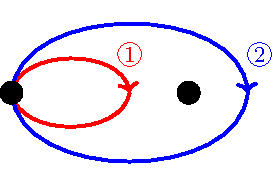
\includegraphics[width=0.35\linewidth]{exchange-paths.pdf}
	\caption{Topological viewpoint of exchange, where Path 1 does not carry out exchange and can be contracted to the pull path, but Path 2 carries out double exchange.}
	\label{fig:exchange}
\end{figure}

Let us now provide a topological picture of exchange, which we'll describe in more detail in the following section.
Consider a system of two indistinguishable electrons arranged as in \autoref{fig:exchange}.
In the figure are also two paths that represent processes that operate on the position of the left particle.
Along Path 1, there is no exchange, as in one sense the particle has not changed its relative position, but more importantly, this path can be contracted (deformed) into the single particle (a null operation, in some sense).

Path 2, on the other hand, corresponds to double exchange, as halfway through, the particles have switched places, and by the end they have switched back.
Moreover, in 3D, it is possible to physically deform path 2 to match path 1 (lift it out of the plane of the paper), so double exchange is equivalent to no exchange.
They have the same topological properties (such paths are called \emph{homotopic}), which admits $e^{2 i \alpha} = 1$, as seen earlier in \autoref{eq:swapped_pm}.

But in 2D, these paths cannot be deformed continuously to match each other, and the paths are knotted!
This means in 2D, double exchange is \emph{not} equivalent to no exchange and that $e^{2 i \alpha}$ does not necessarily equal 1.
This describes a class of particles called \textbf{anyons}, which are the basis for topological quantum computing.\footnote{See the article by V. Lahtinen and J. Pachos, \href{https://arxiv.org/abs/1705.04103}{\emph{SciPost Physics}} 3, 2017, for a lengthier introduction to this topic.}


% % % % % % % % % % % % % % % % % % % % % % % % % % % % % % % % % % % % % 
% % % % % % % % % % % % % % % % % % % % % % % % % % % % % % % % % % % % % 
% % % % % % % % % % % % % % % % % % % % % % % % % % % % % % % % % % % % % 

\section{Topology}

Topology is the study of the \emph{global} properties of geometric objects that don't depend on local features, or are \emph{preserved} under small local deformations.
A canonical example is the topological equivalency of a donut and a mug.
Although the two objects look very different, they are topologically very similar (equivalent, in fact) because both feature a single hole---the donut through the center and the mug through the handle.\footnote{You can read more about topology in \href{https://phys.org/news/2016-10-coffee-donut-topology.html}{this Phys.org article} discussing the \href{https://www.nobelprize.org/prizes/physics/2016/summary/}{2016 Nobel Prize in Physics} on topological phase transitions.}
As a result, it is possible to continuously deform one shape into the other, as seen \href{https://tex.stackexchange.com/questions/210255/torus-to-coffee-mug-homotopy}{in this animation}.
Contrast these two objects with a ball (sphere), which cannot be deformed into either of these shapes without puncturing it, and hence changing its topological properties.
In relation to \autoref{fig:exchange}, we say two objects (or paths) are \textbf{homotopic} to each other if they can be deformed continuously into each other.

How does this apply to the exchange problem we saw in the previous section?
Well, it turns out that if we study fermions from a topological viewpoint, interchanging two objects is topologically like rotating one of them!
This can be seen in an exercise known as \textbf{Dirac's belt trick},\footnote{Also known as \href{https://en.wikipedia.org/wiki/Plate_trick}{Dirac's plate trick}.} in which a belt is straightened so that both ends are the same orientation, e.g., flat.
If we give the buckle end (for easier visualization) a $2\pi$ (\SI{360}{\degree}) twist, there is no way to return the belt to the original orientation as long as both ends remain flat, regardless of how we move the belt in space.
This rotation by $2\pi$ is equivalent to a single exchange.

However, if we rotate the buckle end again by $2\pi$ (we might need a long or soft belt!), so that the total rotation along the length of the belt is $4\pi$, we will find that it is possible to loop the belt once while keeping both ends flat (i.e., a continuous transformation) and return the belt to the original, \emph{untwisted} orientation!
This $4\pi$ rotation is equivalent to double exchange, which we said for indistinguishable particles should result in the same wavefunction, and we see this reflected in the unchanged orientation of the belt.
I encourage you to get a belt (or small object for the plate trick) and try it for yourself!\footnote{This is not just a \emph{Gedankenexperiment}! Take a look at \href{https://www.youtube.com/watch?v=EgsUDby0X1M}{this video} from Trefor Bazett or \href{https://www.gregegan.net/APPLETS/21/21.html}{this applet} for inspiration.}

In the language of topology (advanced!): Rotation through $2\pi$ corresponds to a loop in the group SO(3), but this is not homotopic to the null curve.
On the other hand, the curve associated with a $4\pi$ rotation \emph{is} null-homotopic.

\subsection{Visualization}

\begin{figure}[!ht]
	\centering 
	\includegraphics[width=0.8\linewidth]{topological-shapes.pdf}
	\caption{Visualization of topological shapes. 
	Arrows indicate which edges should be glued together and in which orientation (arrows should be aligned).}
	\label{fig:shapes}
\end{figure}

Here is a visualization I find helpful and it might aid your learning as well.
Imagine we have a rectangular piece of paper that we're trying to transform into a 3D shape.
There are many ways to do this, so to guide the construction, we will draw arrows along opposite edges and their orientation determines how we will join (e.g., glue) the two edges together to turn the 2D paper into a 3D object.
For example, if we only draw upward pointing arrows on the left and right edges of the paper, then joining the two edges will form a cylinder, as illustrated in \autoref{fig:shapes}a.
Closely study the other examples shown to convince yourself that the shapes can be formed as claimed---again, it might be helpful to get some paper and try it!

Left/right $\rightarrow$ cylinder.
Left/right, top/bottom $\rightarrow$ torus.
Left/right with twist $\rightarrow$ M{\"o}bius strip
Left/right, top/bottom, both with twist $\rightarrow$ $\mathbf{RP}^2$, real projective plane.
Hard to visualize!
Yes this is the topological space that defines how indistinguishable particles behave!

We can classify these spaces using something called the \textbf{fundamental group}.\footnote{While long, the \href{https://en.wikipedia.org/wiki/Fundamental_group}{Wikipedia page} on the fundamental group has many nice visuals.}
It classifies the types of curves/paths in a topological space by ``measuring the number of holes" (loosely speaking) in the geometric object.
For example, take the sphere in three dimensions, which we symbolize with $S^2$ (the `2' refers to a 2D surface).

\begin{figure}[!ht]
	\centering 
	\includegraphics[width=0.4\linewidth]{sphere-closed-curve.pdf}
	\caption{Closed curve on sphere.}
	\label{fig:sphere1}
\end{figure}

The blue curve in \autoref{fig:sphere1} (and all closed curves on the sphere) can be contracted to a point on its surface (the null curve).
Therefore, we say that all closed curves are \emph{homotopic} to the null curve, as defined previously.
Using the notation of topology, where the fundamental group is denoted\footnote{`1' for the first homotopy group, $\pi$ likely for its discover, Henri Poincar{\'e}.} by $\pi_1$, we would say 

\begin{equation*}
	\pi_1(S^2) = 0
\end{equation*}

Similarly, if we look at a 2D plane in the Cartesian coordinate system (denoted $R^2$), all closed curves in the plane can also be contracted to a point, and thus there are no holes.
We would denote this in a similar way, 

\begin{equation*}
	\pi_1(R^2) = 0
\end{equation*}

While these examples might not be as tricky, the fundamental group isn't always so trivial.
Consider now the circle in 2D, symbolized by $S^1$, and shown in \autoref{fig:circle1}.

\begin{figure}[!ht]
	\centering 
	\subfloat[]{\includegraphics[width=0.31\linewidth]{circle-null-curve.pdf} \label{fig:circle1a}} \hfill
	\subfloat[]{\includegraphics[width=0.31\linewidth]{circle-1-curve.pdf} \label{fig:circle1b}} \hfill
	\subfloat[]{\includegraphics[width=0.31\linewidth]{circle-2-curve.pdf} \label{fig:circle1c}}
	\caption{Curves on a circle.
	(a) The null curve, which is contractable (homotopic) to a point.
	(b) A knotted curve with a winding number of 1.
	(c) A curve with two loops cannot be contracted to either of the previous two. 
	This path has a winding number of 2.}
	\label{fig:circle1}
\end{figure}

In panel~\ref{fig:circle1a}, we have drawn a small arc that is homotopic to a point when contracted. 
In panel~\ref{fig:circle1b}, we have a single loop around the circle.
This curve is knotted! 
It cannot be contracted to a point, and we quantify its properties using a \emph{winding number} of 1.
Similarly, in panel~\ref{fig:circle1b}, we have two loops around the circle.
This is yet another distinct case, as there's no way to contract this double loop into a single loop or the null curve. 
In fact, we can characterize it with a winding number of 2.

By now you probably see the pattern. 
The \href{https://en.wikipedia.org/wiki/Winding_number}{winding number} can be positive or negative depending on whether the loops are counterclockwise or clockwise around the circle, respectively.
Thus we can have a distinct loop/curve for every positive or negative integer.
We say that $\pi_1(S^2) = \mathbb{Z}$, which is the group of integers.
In this way, the fundamental group is powerful because it lets us classify different topological spaces using an algebraic quantity.

\begin{figure}[!ht]
	\centering 
	\subfloat[]{\includegraphics[width=0.35\linewidth]{sphere-1-hole.pdf} \label{fig:sphere2a}} \hspace{6ex}
	\subfloat[]{\includegraphics[width=0.35\linewidth]{sphere-2-hole.pdf} \label{fig:sphere2b}}
	\caption{(a) A punctured sphere with a single hole, where all loops on the surface are trivial.
	(b) A double-punctured sphere, where the same loop is no longer trivial.}
	\label{fig:sphere2}
\end{figure}

Let's do a few more examples. 
Consider the \emph{punctured} sphere, which is a sphere with a hole cut in it (Figure~\ref{fig:sphere2a}).
All loops, even those which enclose the hole (example shown in blue) are trivial.
Such a loop can be expanded outward and then collapsed on the \emph{other side} of the sphere!
Indeed, the punctured sphere is \emph{homeomorphic}\footnote{This is similar to homotopy equivalence, but \href{https://en.wikipedia.org/wiki/Homotopy\#Homotopy_equivalence_vs._homeomorphism}{slightly stronger}. Sorry for so many terms!} to a disc $D^2$.
There exists a continuous deformation which collapses a punctured sphere to a flat 2D disc.
Note here we use a different notation because a disc includes all the points inside the circle, whereas the circle $S^1$ is just the boundary.

Figure~\ref{fig:sphere2b} is another example, this time a double punctured sphere.
Now a loop around one hole gets caught on the other during the attempted collapse of the loop.
In fact, this space is homeomorphic to a punctured disc, which in turn is just the circle $S^1$!\footnote{Can you picture this? What if you start with an annulus and then make it thinner?} 
Thus the fundamental group of the twice-punctured sphere is also $\mathbb{Z}$.


% % % % % % % % % % % % % % % % % % % % % % % % % % % % % % % % % % % % % 
% % % % % % % % % % % % % % % % % % % % % % % % % % % % % % % % % % % % % 
% % % % % % % % % % % % % % % % % % % % % % % % % % % % % % % % % % % % % 

\section{Back to fermions}

That was exciting! (hopefully)
Time to bring back the science.
In 3D, let's consider the 2-particle configuration space for fermions.
We can define this by the relative coordinate $\vec{r} = \vec{r}_1 - \vec{r}_2$, where $\vec{r}_1$ and $\vec{r}_2$ are vectors pointing at the two particles (i.e., their positions).
By the Pauli exclusion principle, we know that $\vec{r} \neq 0$.

Furthermore, let's consider for simplicity (and without loss of generality\footnote{Theorists use this phrase when constructing an argument that uses a specific example or assumptions, but the result is generally valid, as other possible assumptions are equivalent by symmetry.}) the case where $\abs{\vec{r}}$ is fixed (topology allows for continuous deformations to enable this).
Then we would have a sphere!

\begin{figure}[!ht]
	\centering 
	\subfloat[]{\includegraphics[width=0.4\linewidth]{sphere-antipodes.pdf}} \hspace{5ex} 
	\subfloat[]{\includegraphics[width=0.42\linewidth]{sphere-antipodes-null-curve.pdf}}
	\caption{Antipodes on a sphere.}
	\label{fig:sphere3}
\end{figure}

Now let's look at the setup in \autoref{fig:sphere3}a, where $\vec{r}$ and $-\vec{r}$ are \textbf{antipodal points} on the sphere.
If we let $\vec{r} = \vec{r}_1 - \vec{r}_2$, which again we can always get by manipulating the particles' positions, then exchanging the two particles would produce $-\vec{r}$.

If the particles are indistinguishable, then the topological space we have for this 2-particle system is a sphere with antipodal points identified.\footnote{Which, as alluded to before, is the definition of the space RP$^2$, as explained nicely \href{https://www.popmath.org.uk/sculpmath/pagesm/plane.html}{here}.}

Now we might ask: What is this space?
Let's revisit our original activity by considering paths in this space that represent the motion of the two particles, such as the red path in \autoref{fig:sphere3}b.
We've already seen how such a path is homotopic to the null loop as it can be collapsed to a point.

\begin{figure}[!ht]
	\centering 
	\includegraphics[width=0.4\linewidth]{sphere-single-exchange.pdf}
	\caption{Single exchange on a sphere.}
	\label{fig:sphere-exchange}
\end{figure}

Now consider the path in \autoref{fig:sphere-exchange}, which sends $\vec{r} \rightarrow -\vec{r}$ and corresponds to an exchange.
It is a closed loop in this space!
We travel from $A$ to $B$ along the curve, and then because $B$ is identical to $A$, we go through a portal back to $A$! 
This curve cannot be contracted to a point while keeping the ends fixed.
This is the path associated with an exchange operation, or rotation by $2\pi$.

\begin{figure}[!ht]
	\centering 
	\includegraphics[width=0.4\linewidth]{sphere-double-exchange-top.pdf}
	\caption{Double exchange on a sphere. (top view)}
	\label{fig:sphere-double}
\end{figure}

Next, let's consider double exchange, which we draw in \autoref{fig:sphere-double}. 
Again we begin by traveling from $A$ to $B$, which sends us back to $A$.
This time, we label this new (equivalent) point $C$.
Now we travel from $C$ to $D$, where the latter is equivalent to the original point $B$. 
This is the loop associated with double exchange, or a rotation by $4\pi$.

\begin{figure}[!ht]
	\centering 
	\subfloat[]{\includegraphics[width=0.23\linewidth]{sphere-double-exchange-1.pdf} \label{fig:sphere-double2a}} \hfill
	\subfloat[]{\includegraphics[width=0.23\linewidth]{sphere-double-exchange-2.pdf} \label{fig:sphere-double2b}} \hfill
	\subfloat[]{\includegraphics[width=0.23\linewidth]{sphere-double-exchange-3.pdf} \label{fig:sphere-double2c}} \hfill
	\subfloat[]{\includegraphics[width=0.23\linewidth]{sphere-double-exchange-4.pdf} \label{fig:sphere-double2d}}
	\caption{Double exchange process on a sphere.}
	\label{fig:sphere-double2}
\end{figure}

How might we perform a continuous deformation of this closed double loop from $A$ to $D$?
\autoref{fig:sphere-double2} attempts to illustrate this process.
We start with the configuration in \ref{fig:sphere-double2a} and we move points $B$ and $C$ along the equator in opposite directions, away from $D$ and $A$, respectively (\ref{fig:sphere-double2b}). 
Note that during this process, $B$ and $C$ remain antipodes and $A$ and $D$ are fixed in place, so we have not broken the topology of the system; such a continuous deformation was not possible previously when we only had $A$ and $B$ as endpoints (\ref{fig:sphere-exchange}).
We proceed with this process until $B$ coincides with $A$ and $C$ coincides with $D$, effectively closing two smaller loops on the surface of the sphere (\ref{fig:sphere-double2c}). 
Finally, in a feat of quantum magic, we pull the loop at $A$,$B$ through the antipodal portal to the other side, resulting in panel \ref{fig:sphere-double2d}.
Now we have a trivial, contractable loop $ABCD$ that is homotopic to null.
Thus there are only 2 classes of topologically inequivalent closed paths in 3D, corresponding to fermions and bosons.
In topology notation, we write $\pi_1(\mathrm{RP}^2) = \mathbb{Z}_2$, where $\mathbb{Z}_2$ denotes the cyclic group of order 2.\footnote{Sometimes $\mathbb{Z}_2$ is also written as $\mathbb{Z}/2\mathbb{Z}$.}
This means that the group can be generated using just two elements of its members, $I$ and $X$, with $X^2 = I$.
We have now arrived back to the beginning of the chapter, with a much more complex, topological view of the statement $e^{2i \alpha} = 1$!

\begin{figure}[!ht]
	\centering 
	\subfloat[]{\includegraphics[width=0.4\linewidth]{circle-single-exchange.pdf} \label{fig:circle-exchange-a}} \hspace{6ex}
	\subfloat[]{\includegraphics[width=0.4\linewidth]{circle-double-exchange.pdf} \label{fig:circle-exchange-b}}
	\caption{Antipodes on a circle.}
	\label{fig:circle-exchange}
\end{figure}

Before we wrap up, let's go down a dimension into 2D.
This configuration space is a circle with opposite points identified (RP$^1$).
As illustrated in Figure~\ref{fig:circle-exchange-a}, the path $A \rightarrow B$ is a closed loop (as $A$ and $B$ are antipodes) and corresponds to the exchange operation in 2D.
Performing double exchange takes us all the way around the circle, as shown in panel~\ref{fig:circle-exchange-b}.
Note this is still topologically distinct.

Generalizing, under $n$ exchanges, we just wrap $n$ times around.
The winding number is $n$ and just like above, we can say $\pi_1 (\mathrm{RP}^1) = \mathbb{Z}$.
Thus, if we pick up a phase factor $e^{i\alpha}$ on each exchange, there is no requirement that $e^{2i \alpha} = 1$.
This is the anyon case!


\subsection{Notes on spin statistics}

In the previous discussion, the essence of the argument comes down to the following picture (Figure~\ref{fig:loop-twist-a}).
In 3D, it would seem that the left loop is equivalent to the right.
If we just pull on it, it straightens out, as one might expect with a string.

\begin{figure}[!ht]
	\centering 
	\subfloat[]{\includegraphics[height=2.5in]{twist-thin.pdf} \label{fig:loop-twist-a}} \hspace{8ex} 
	\subfloat[]{\includegraphics[height=2.5in]{twist-thick.pdf} \label{fig:loop-twist-b}}
	\caption{Twisted loops thin and thick.}
	\label{fig:loop-twist}
\end{figure}

In fact, however, these two objects are \emph{not} topologically equivalent.
Imagine a string with finite diameter (Figure~\ref{fig:loop-twist-b}).
If we try to pull this string straight, the loop is gone, yes, but we would also get a double twist along the length of the string.\footnote{A similar thing happens if we try to straighten a garden hose.}
This is the fact that underlies how we get nontrivial phases under exchange.


Our motivation for studying the fundamental group is to prove that the fundamental group of $SO(3)$, the group of rotations, is a cyclic group of order two. 
In physics applications this result is interesting to us because it is associated to spin and spinor representations in quantum mechanics. 
It explains why a rotation body can have a spin of half a quantum and no other fraction.



% % % % % % % % % % % % % % % % % % % % % % % % % % % % % % % % % % % % % 
% % % % % % % % % % % % % % % % % % % % % % % % % % % % % % % % % % % % % 
% % % % % % % % % % % % % % % % % % % % % % % % % % % % % % % % % % % % % 

\section{Application: Topological insulators}

TODO. 
If you've stuck with us all the way to this point, major kudos.

https://www.youtube.com/watch?v=6ebiyOtn7NA knots video applications

Joel Moore, Nature: https://www.nature.com/articles/nature08916
Qi and Zhang, Rev Modern Phys: https://link.aps.org/doi/10.1103/RevModPhys.83.1057
Hasan and Kane, Rev Modern Phys: https://link.aps.org/doi/10.1103/RevModPhys.82.3045
Ando, intro, Japan: https://journals.jps.jp/doi/abs/10.7566/JPSJ.82.102001
Choi, true intro, IEEE Spectrum: https://spectrum.ieee.org/a-beginners-guide-to-topological-materials

Electronic topological insulators: bismuthene.

Photonic topological insulators: Layers of GaAs and AlGaAs.

Topological superconductors: superconducting metal + semiconductor, producing Majorana fermions.

Topological semimetals: TaAs, CoSi, Dirac semimetals, Weyl semimetals, etc.


% % % % % % % % % % % % % % % % % % % % % % % % % % % % % % % % % % % % % 
% % % % % % % % % % % % % % % % % % % % % % % % % % % % % % % % % % % % % 
% % % % % % % % % % % % % % % % % % % % % % % % % % % % % % % % % % % % % 

\section{Summary}
To recap, in this chapter we analyzed...

%} % for doublespacing
\end{document}	% Topology and indistringuishability

%% Created: Enze Chen, June 2025
%
% Chapter 11 of the MSE 142 coursereader. This chapter introduces ideas in quantum computing as an advanced extension of the course themes.

% Uncomment the following three lines and last line to individually compile this chapter
\documentclass[12pt, english]{book}
\usepackage{142crstyle}
\begin{document}

\chapter[Quantum computing]{Work in Progress:\\Quantum Computing} \label{ch:computing}
%{ \doublespacing 
As an advanced topic, we'll discuss the advantages of quantum computing.


For more information, see this article: https://dl.acm.org/doi/10.1145/367701.367709
or this book: https://doi.org/10.1093/oso/9780192857972.001.0001


%%%%%%%%%%%%%%%%%%%%%%%%%%%%%%%%%%%%%%%%%%%%%%%%%%%%%%%%%%%%%%%%%%%%%%%%%%%%%%%%

\section{Before you begin}

This chapter builds on the following concepts, some of which we've already discussed in class, others you will likely have encountered elsewhere.
We include links to resources that may aid your review, as mastery of these concepts will allow you to get the most out of this chapter.

\begin{itemize}
	\item foo 
	\item bar 
	\item Prerequisite self-check quiz 
\end{itemize}


%%%%%%%%%%%%%%%%%%%%%%%%%%%%%%%%%%%%%%%%%%%%%%%%%%%%%%%%%%%%%%%%%%%%%%%%%%%%%%%%


\section{Introduction to formalisms}

Imagine a general two-level system, which could represent spin states or a light-activated system, that we will represent as $\ket{0}$ and $\ket{1}$.
We could write them in a different way, in vector notation, as follows:

\begin{equation*}
	\ket{0} = \begin{pmatrix} 1 \\ 0 \end{pmatrix}, \qquad \ket{1} = \begin{pmatrix} 0 \\ 1 \end{pmatrix} 
\end{equation*}

These are the basis states, similar to our discussion of polarization in Chapter 1.
To help visualize their linear independence, we could even draw them being orthogonally arranged on the page (e.g., aligned with the $x$- and $y$-axis, respectively), but in no sense do these states have any real-space directions!

Given the basis states $\ket{0}$ and $\ket{1}$, we can write the general superposition state as 

\begin{equation*}
	\ket{\psi} = \alpha \ket{0} + \beta \ket{1},
\end{equation*}

where $\alpha$ and $\beta$ are coefficients such that $\abs{\alpha}^2 + \abs{\beta}^2 = 1$.
An example superposition state is $\ket{\psi} = \dfrac{1}{\sqrt{2}} \left( \ket{0} + \ket{1} \right)$, where we note that $\abs{\psi} = 1$.

Now imagine we have a system with two qubits.
We can represent the states of this system as $\ket{q_1 q_2}$, where $q_i$ represents the state of the $i$th qubit.
For example, $\ket{00}$ would represent qubits 1 and 2 both in the \texttt{0} state.
Continuing in the framework of the vector notation from before, we can express all four possible states as

\begin{equation*}
	\ket{00} = \begin{pmatrix} 1 \\ 0 \\ 0 \\ 0 \end{pmatrix}, \qquad 
	\ket{01} = \begin{pmatrix} 0 \\ 1 \\ 0 \\ 0 \end{pmatrix}, \qquad 
	\ket{10} = \begin{pmatrix} 0 \\ 0 \\ 1 \\ 0 \end{pmatrix}, \qquad 
	\ket{11} = \begin{pmatrix} 0 \\ 0 \\ 0 \\ 1 \end{pmatrix}
\end{equation*}

where we have four unit vectors that comprise an orthogonal basis set in a 4-dimensional space.
Thus we can encode using binary notation the equal-weighted two-qubit state and express it as

\begin{equation*}
	\ket{\psi} = \frac{1}{2} \left( \ket{00} + \ket{01} + \ket{10} + \ket{11} \right) = \frac{1}{2} \left( \ket{0} + \ket{1} + \ket{2} + \ket{3} \right)
\end{equation*}

More generally, we could say that $\ket{\psi} = \dfrac{1}{\sqrt{2^n}} \displaystyle\sum_{x=0}^{2^n-1} \alpha_x \ket{x}$.

If we continue in this vein, we will find that for $n$ qubits there are $2^n$ possibilities!
Encodes $2^n$ numbers. 
How large is this? 
Well, for $n \sim 270$, $2^n$ would be larger than the number of atoms in the universe!\footnote{Which current estimates place at $10^{80}$, see the \href{https://en.wikipedia.org/wiki/Eddington_number}{Eddington number}.}
It would be quite remarkable to store all this information in just 200 atoms!
Even a more modest number like $n = 100$ would give us $10^{30}$ bits, which is equal to $\sim 10^{29}$ or 1 billion zettabytes. 
The global datasphere is only 150 zettabytes (but quickly growing)!
If we could implement a function on this superposition state, then the function would be evaluated on all inputs in parallel.

\begin{equation*}
	\ket{\psi} \rightarrow \boxed{f} \rightarrow \dfrac{1}{\sqrt{2^n}} \sum_{x=0}^{2^n-1} \alpha_x \ket{x}
\end{equation*}

where $f$ is a quantum gate.
The assumption here is that we have a linear operator. 
Actually: operators are unitary and reversible.

But there's a problem: If we make a measurement, we get a single number!
The superposition state collapses, as we saw earlier in the course.
There is no obvious way to sample coefficients.

Perhaps... we can try to be clever and make many copies and then measure many times to sample?
Unfortunately not---the quantum no-cloning theorem!

\textbf{Put the definition box for no-cloning theorem here}

We'll sketch the idea for this theorem below.
Suppose there is an operator $U$ that is linear (and unitary) that can clone an arbitrary state $\ket{\psi} = \alpha \ket{0} + \beta \ket{1}$.
We would have the configuration picture in \autoref{fig:no-clone-1}.

\begin{figure}[!ht]
	\centering
	\includegraphics[width=0.6\linewidth]{no-clone-1.pdf}
	\caption{Caption}
	\label{fig:no-clone-1}
\end{figure}

But 
\begin{align*}
	\ket{\psi} \ket{\psi} &= \left( \alpha \ket{0} + \beta \ket{1} \right) \otimes \left( \alpha \ket{0} + \beta \ket{1} \right) \\
	&= \alpha^2 \ket{00} + \alpha \beta \ket{01} + \beta \alpha \ket{10} + \beta^2 \ket{11}
\end{align*}

But on the other hand, 
\begin{align*}
	U \left( \ket{\psi} \ket{0} \right) &= U \left( \alpha \ket{0} + \beta \ket{1} \right) \ket{0} \\ 
	&= \alpha U \ket{00} + \beta U \ket{1} \ket{0} \\
	&= \alpha \ket{00} + \beta \ket{11}
\end{align*}

and the cross terms are missing.
This means cloning is impossible! 

For a different proof, suppose there exists a unitary cloning operator $U$.
This would satisfy 
\[ \ket{\psi 0} \stackrel{U}{\rightarrow} \ket{\psi \psi}\ \text{for all}\ \psi \]

Thus, $U \ket{00} = \ket{00}$ and $U\ket{10} = \ket{11}$.
If we apply this to $H \ket{0} = \frac{1}{\sqrt{2}} \left( \ket{0} + \ket{1} \right)$, we get $U \frac{1}{\sqrt{2}} \left( \ket{0} + \ket{1} \right) \ket{0} = \frac{1}{\sqrt{2}} \left( \ket{00} + \ket{11} \right)$ by linearity.

But this is not successfully cloned, since it should equal
\[ \frac{1}{2} \left( \ket{0} + \ket{1} \right) \left( \ket{0} + \ket{1} \right) = \frac{1}{2} \left( \ket{00} + \ket{01} + \ket{10} + \ket{11} \right) \]
Therefore, $U$ does not exist.


\section{Allowed operators}

So what kind of operators are allowed?
For quantum logic gates, we have
\begin{itemize}
	\item The simplest example is $H$ that satisfies $H \ket{\psi} = i \hbar \pdv{t} \ket{\psi}$ which gives time evolution.
	
	\item \texttt{NOT} (or $X$ gate), which maps $\ket{0} \rightarrow \ket{1}$ and $\ket{1} \rightarrow \ket{0}$.
	The matrix representation of this is $\begin{pmatrix} 0 & 1 \\ 1 & 0 \end{pmatrix}$, so $\begin{pmatrix} 0 & 1 \\ 1 & 0 \end{pmatrix} \begin{pmatrix} 1 \\ 0 \end{pmatrix} = \begin{pmatrix} 0 \\ 1 \end{pmatrix}$.
	
	\item $Z$ gate, which maps $\ket{0} \rightarrow \ket{0}$ but $\ket{1} \rightarrow -\ket{1}$.
	Written out more fully, $Z \left( \alpha \ket{0} + \beta \ket{1} \right) \rightarrow \alpha \ket{0} - \beta \ket{1}$, which induces a phase flip. 
	The matrix representation of this gate is $\begin{pmatrix} 1 & 0 \\ 0 & -1 \end{pmatrix}$.
\end{itemize}


\section{Bloch sphere}

Another way to visualize the qubit state is on a construct called the \textbf{Bloch sphere} (\autoref{fig:bloch-sphere}), which has $\ket{0}$ and $\ket{1}$ on the north and south pole, respectively, and all possible qubit states represented on the surface of the sphere.
Note that classical bits are restricted to exactly $\ket{0}$ or $\ket{1}$, but quantum allows everything in between.

\begin{figure}[!ht]
	\centering
	\subfloat[]{\includegraphics[width=0.3\linewidth]{bloch-sphere-1.pdf}} \hspace{10ex}
	\subfloat[]{\includegraphics[width=0.3\linewidth]{bloch-sphere-2.pdf}}
	\caption{(a) Bloch sphere. (b) explicit $xyz$ coordinates.}
	\label{fig:bloch-sphere}
\end{figure}

As before, a single qubit can be represented by $\ket{\psi} = \alpha \ket{0} + \beta \ket{1}$, where $\abs{\alpha}^2 + \abs{\beta}^2 = 1$.
Note that although $\alpha$, $\beta$ can be imaginary, so it seems like we have four undetermined values, we only care about their relative phase.
So the most general representation for the state is in fact $\ket{\psi} = r_{\alpha} \ket{0} + r_{\beta} e^{i \phi} \ket{1}$.

If we apply the normalization criteria, we find:
\begin{align*}
	\braket{\psi}{\psi} &= 1 \\
	\ket{\psi} &= r_{\alpha} \ket{0} + (x + iy) \ket{1} \\
	\braket{\psi}{\psi} = r_{\alpha}^2 + x^2 + y^2 &= 1 \\
\end{align*}
which returns the equation for the unit sphere.

The usual parameterization for $\psi$ is $\ket{\psi} = \cos \frac{\theta}{2} \ket{0} + \sin \frac{\theta}{2} e^{i \phi} \ket{1}$.
This leads to the following convenient values:

\begin{align*}
	\theta = 0  &\rightarrow  \ket{0} \\
	\theta = \pi  &\rightarrow  \ket{1} \\
	\theta = \frac{\pi}{2}, \phi = 0  &\rightarrow  \ket{X} = \frac{1}{\sqrt{2}} \left( \ket{0} + \ket{1} \right) \\
	\theta = \frac{\pi}{2}, \phi = \frac{\pi}{2}  &\rightarrow  \ket{Y} = \frac{1}{\sqrt{2}} \left( \ket{0} + i\ket{1} \right) \\
\end{align*}

Logic gates represent motion on the surface.
For example, the \texttt{NOT} gate is given by $R(\pi)$ or rotation by $\pi = \SI{180}{\degree}$.

Another allowed quantum gate is the \textbf{Hadamard gate}, $H$, which maps

\begin{align*}
	\ket{0} &\rightarrow \frac{1}{\sqrt{2}} \left( \ket{0} + \ket{1} \right) = \ket{+} \\
	\ket{1} &\rightarrow \frac{1}{\sqrt{2}} \left( \ket{0} - \ket{1} \right) = \ket{-}
\end{align*}

In matrix representation, this is expressed as 

\[ H = \frac{1}{\sqrt{2}} \begin{pmatrix} 1 & 1 \\ 1 & -1 \end{pmatrix}\ \text{so}\ H \begin{pmatrix} 1 \\ 0 \end{pmatrix} = \begin{pmatrix} 1 & 1 \\ 1 & -1 \end{pmatrix} \begin{pmatrix} 1 \\ 0 \end{pmatrix} = \frac{1}{\sqrt{2}} \begin{pmatrix} 1 \\ 1 \end{pmatrix} \]

This generates equally weighted superposition states.
It is visualized as a rotation by $\pi/2$.

\section{2-qubit gates}

Consider the following setup:

\begin{figure}[!ht]
	\centering
	\includegraphics[height=0.8in]{cnot-1.pdf}
	\caption{CNOT gate}
	\label{fig:cnot-1}
\end{figure}

We'll now consider the \texttt{CNOT} operation (\autoref{fig:cnot-1}) which performs \texttt{NOT} on the second qubit only when the first qubit is 1.
That is, we have

\begin{align*}
	\ket{00} &\rightarrow \ket{00} \\
	\ket{01} &\rightarrow \ket{01} \\
	\ket{10} &\rightarrow \ket{11} \\
	\ket{11} &\rightarrow \ket{10} 
\end{align*}

In the matrix representation,

\[ U = \begin{pmatrix} 1 & 0 & 0 & 0 \\ 0 & 1 & 0 & 0 \\ 0 & 0 & 0 & 1 \\ 0 & 0 & 1 & 0 \end{pmatrix} \begin{pmatrix} 0 \\ 0 \\ 0 \\ 1 \end{pmatrix} = \begin{pmatrix} 0 \\ 0 \\ 1 \\ 0 \end{pmatrix} \]

\begin{figure}[!ht]
	\centering
	\includegraphics[height=0.8in]{cnot-2.pdf}
	\caption{Caption}
	\label{fig:cnot-2}
\end{figure}

\autoref{fig:cnot-2} has a simplified example of such a configuration.
On the control side, $\ket{0} \stackrel{H}{\rightarrow} \frac{1}{\sqrt{2}} \left( \ket{0} + \ket{1} \right)$.
For the target, $\ket{0} \rightarrow \frac{1}{\sqrt{2}} \left( \ket{00} + \ket{11} \right)$.
This is a maximally entangled state: If we measure qubit 1 ($Q_1$), we would get 0,1 with \SI{50}{\percent} probability.

Here's a thought experiment that reveals something interesting about this construction.
Suppose Alice takes $Q_1$ and Bob takes $Q_2$ and goes to Mars.
Now if Alice measures $Q_1$ to be $\ket{0}$, she instantly knows what Bob will measure, since the measurements are correlated.

But now suppose Alice first applies $H$ to her qubit, to get

\[ (H \otimes I) \frac{1}{\sqrt{2}} \left( \ket{00} + \ket{11} \right) = \frac{1}{2} \left( \ket{00} + \ket{10} + \ket{01} - \ket{11} \right) \]

Now if Alice measures $\ket{0}$, Bob's qubit collapses to $\frac{1}{\sqrt{2}} \left( \ket{0} + \ket{1} \right) = \ket{+}$.
But if Alice measures $\ket{1}$, Bob's qubit instantly goes to $\frac{1}{\sqrt{2}} \left( \ket{0} - \ket{1} \right) = \ket{-}$.
This is the signature of the famous EPR paradox.\footnote{Named after its formulators: Einstein, Podolsky, and Rosen, \href{https://link.aps.org/doi/10.1103/PhysRev.47.777}{\emph{Phys. Rev. Lett.}} 47, 1935.}

What is the quantum parallelism? 
Imagine we have a black box that takes input $x$ and outputs $f(x)$.
$x$ can take on values 0 and 1, as can $f(x)$.
We want to know if $f(0) = f(1)$ (constant) or $f(0) \neq f(1)$ (balanced).
Classically, we would need to measure both $f(0)$ and $f(1)$, but our box is so slow that each computation takes \SI{24}{\hour}. 
Instead, consider the following quantum gate (\texttt{CNOT}) in \autoref{fig:cnot-3}:

\begin{figure}[!ht]
	\centering
	\includegraphics[width=0.4\linewidth]{cnot-3.pdf}
	\caption{Caption}
	\label{fig:cnot-3}
\end{figure}

where the $\oplus$ symbol represents addition modulo 2, and the result is that the second bit is flipped only if $f$ acting on the first qubit is 1 (otherwise does nothing).
Written out, this is 

\[ U: \ket{x,y} \rightarrow \ket{x, y \oplus f(x)} \]

To this machine we input the superposition state for the second qubit, $\frac{1}{\sqrt{2}}\left( \ket{0} - \ket{1} \right)$.
This would return:

\[ U: \ket{x, \frac{1}{\sqrt{2}} (\ket{0} - \ket{1})} \rightarrow \ket{x} \frac{1}{\sqrt{2}} (\ket{f(x)} - \ket{1 \oplus f(x)}) = \ket{x} (-1)^{f(x)} \frac{1}{\sqrt{2}} ( \ket{0} - \ket{1} )\]

and so $f$ determines the phase of the output! 

OK, so now let's consider making the first qubit also a superposition:

\begin{align*}
	U: \ket{\frac{1}{\sqrt{2}} (\ket{0} - \ket{1}), \frac{1}{\sqrt{2}} (\ket{0} - \ket{1})} &\rightarrow 
	\frac{1}{2} \left( U \ket{0} (\ket{0} - \ket{1}) + U \ket{1} (\ket{0} - \ket{1}) \right) \\
	&= \frac{1}{2} \left[ (-1)^{f(0)} \ket{0} + (-1)^{f(1)} \ket{1} \right]  (\ket{0} - \ket{1}) \\
\end{align*}

\begin{figure}[!ht]
	\centering
	\subfloat[]{\includegraphics[height=0.7in]{epr-1.pdf}} \hspace{10ex}
	\subfloat[]{\includegraphics[height=1.8in]{epr-2.pdf}}
	\caption{EPR paradox}
	\label{fig:epr}
\end{figure}

We illustrate this in \autoref{fig:epr}.
Now we apply the Hadamard operator on the first qubit:

\begin{align*}
	H \left[ (-1)^{f(0)} \ket{0} + (-1)^{f(1)} \ket{1} \right] &\rightarrow
	(-1)^{f(0)} (\ket{0} + \ket{1}) + (-1)^{f(1)} (\ket{0} - \ket{1}) \\
	&= \left( (-1)^{f(0)} + (-1)^{f(1)} \right) \ket{0} + \left( (-1)^{f(0)} - (-1)^{f(1)} \right) \ket{1}
\end{align*}

And now we try to make a measurement in the $\ket{0}$, $\ket{1}$ basis. 
If $f(0) = f(1)$ (constant), then we always measure $\ket{0}$ with a \SI{100}{\percent} probability.
On the other hand, if $f(0) \neq f(1)$ (balanced), then we always measure $\ket{1}$.
This is the quantum parallelism, and it shows how one can manipulate states to determine measurement outcomes. 

\section{Quantum teleportation}

Now let's see how we can take advantage of entanglement. 
We'll start with a EPR pair: $\frac{1}{\sqrt{2}} (\ket{00} + \ket{11})$.
Recall we can generate this using the protocol in \autoref{fig:cnot-2}.
Alice takes the first qubit, while Bob takes the 2nd one and travels.
Now Alice wants to deliver a qubit $\ket{\psi}$ to Bob, where $\ket{\psi} = \alpha \ket{0} + \beta \ket{1}$.
Note the following:

\begin{itemize}
	\item Alice doesn't know the state of the qubit she wants to send!
	
	\item If she measured it, she would just measure one state, which is not enough to reconstruct the wavefunction.
	
	\item Even if she did know $\ket{\psi}$, it would take infinite information to send! 
	(recall $\alpha$ and $\beta$ are continuous)
	
	\item Yet we will show she can teleport quantum state with 2 bits of information!
	
	\item If an observer intercepts the qubit, the information is useless.
	We need the second qubit as a key to decode.
	Thus Alice doesn't need to know where Bob is! 
	She just has to broadcast the information.
\end{itemize}

\begin{figure}[!ht]
	\centering
	\includegraphics[width=\linewidth]{three-qubit.pdf}
	\caption{Three-qubit problem.}
	\label{fig:three-qubit}
\end{figure}

\autoref{fig:three-qubit} presents the 3-qubit problem, where Alice has two of them.
The input ``s a $\ket{\psi_o}$" equals

\[ \ket{\psi} \ket{\beta_{00}} = \left( \alpha \ket{0} + \beta \ket{1} \right) \otimes \frac{1}{\sqrt{2}} \left( \ket{00} + \ket{11} \right) = \frac{1}{\sqrt{2}} \left( \alpha \ket{000} + \alpha \ket{011} + \beta \ket{100} + \beta \ket{111} \right) \]

After \texttt{CNOT}, $\ket{\psi_1} = \frac{1}{\sqrt{2}} \left( \alpha \ket{000} + \alpha \ket{011} + \beta \ket{110} + \beta \ket{101} \right)$.

After $H$, $\ket{\psi_2} = \frac{1}{2} \left( \alpha \ket{000} + \alpha \ket{100} + \alpha \ket{011} + \alpha \ket{111} + \beta \ket{01} - \beta \ket{110} + \beta \ket{001} - \beta \ket{101} \right)$.

Now Alice measures her qubit and send the result to Bob.
The outcomes are summarized in \autoref{tab:three-qubit}.

\begin{table}[!ht]
	\centering
	\begin{tabular}{cc}
		If Alice sees: & Then Bob's qubit is: \\
		\toprule 
		$\ket{00}$ & $\alpha \ket{0} + \beta \ket{1}$ \\
		$\ket{1}$ $\ket{10}$ & $\alpha \ket{1}$ $\beta \ket{0}$ $\alpha \ket{0} - \beta \ket{1}$ \\
		$\ket{11}$ & $\alpha \ket{1} - \beta \ket{0}$
	\end{tabular}
	\caption{Caption}
	\label{tab:three-qubit}
\end{table}

Teleportation is complete if $\ket{00}$ is measured.
If $\ket{01}$ is measured, Bob just applies $X$ gate.
If $\ket{10}$ is measured, apply $Z$ gate.
If $\ket{11}$ is measured, apply both $X$ and $Z$.

\section[General comments]{General comments on entanglement}

For a single spin, the basis is $\ket{\uparrow}$ and $\ket{\downarrow}$.
A superposition state is composed of $c_{\uparrow} \ket{\uparrow} + c_{\downarrow} \ket{\downarrow}$.

For two spins, the basis is $\ket{\uparrow} \ket{\uparrow}$, $\ket{\uparrow} \ket{\downarrow}$, $\ket{\downarrow} \ket{\uparrow}$, and $\ket{\downarrow} \ket{\downarrow}$.
In this case, the general superposition state would be $a \ket{\uparrow \uparrow} + b \ket{\uparrow \downarrow} + c \ket{\downarrow \uparrow} + d \ket{\downarrow \downarrow}$.

The Key point: This general superposition state of two qubits cannot generally be written as the product $\left( c_{\uparrow}^1 \ket{\uparrow} + c_{\downarrow}^1 \ket{\downarrow} \right) \left( c_{\uparrow}^2 \ket{\uparrow} + c_{\downarrow}^2 \ket{\downarrow} \right)$.
In other words, one cannot say spin 1 is in one state and spin 2 is in another.
Rather, they are \textbf{entangled}.

For example, the product $\ket{\uparrow} \ket{\downarrow}$ is \emph{entangled}.
This is because $\ket{\uparrow \downarrow} + \ket{\downarrow \downarrow} = \left( \ket{\uparrow} + \ket{\downarrow} \right) \ket{\downarrow}$ is not entangled.
Here, the second spin is definitely down.

But $\ket{\uparrow \uparrow} + \ket{\downarrow \downarrow}$ or $\ket{\uparrow \downarrow} - \ket{\downarrow \uparrow}$ are. 
We can't say what state spin 1 is in.
A measurement gives up or down with \SI{50}{\percent} probability, but there are hidden correlations.

Black hole entanglement: Ads/LET: Linkage between entanglement and gravity.

ER : EPR : Wormhole = 2 entangled black holes.

Can we test quantum gravity in the laboratory via the creation of entangled states?


%%%%%%%%%%%%%%%%%%%%%%%%%%%%%%%%%%%%%%%%%%%%%%%%%%%%%%%%%%%%%%%%%%%%%%%%%%%%%%%%

\section[Applications]{Application: Superconducting qubits or spin qubits in Si}

Superconducting Qubits: Superconducting materials are among the most widely used implementations of qubits. You can explore how materials such as niobium and aluminum are employed to create Josephson junctions, essential for superconducting qubits. Discuss the quantum coherence of these materials and how their superconducting properties enable low-resistance pathways, crucial for creating stable qubit states that elevate the performance of quantum processors.

Spin Qubits in Silicon: Highlight how silicon, a well-known semiconductor, is being explored for encoding qubits using the spin of electrons or nuclei. You can cover topics on how impurities in silicon can be utilized to create qubit systems and the ongoing research to integrate quantum computing with classical silicon-based technology. Discussing the material's advantages (like the existing fabrication infrastructure from classical computing) could also resonate well with students.

N-V centers in diamond?


%%%%%%%%%%%%%%%%%%%%%%%%%%%%%%%%%%%%%%%%%%%%%%%%%%%%%%%%%%%%%%%%%%%%%%%%%%%%%%%%

\section{Summary}
To recap, in this chapter we analyzed...

%} % for doublespacing
\end{document}	% Quantum computing

% % % % % % % % % % % % % % % % % % % % % % % % % % % % % % % % % % % % % 
% % % % % % % % % % % % % % % % % % % % % % % % % % % % % % % % % % % % % 

\appendix

% Created: Enze Chen, May 2017

% Appendix A of the MSE 142 coursereader. 
% This chapter serves as a reference sheet for physical constants, SI prefixes, the Schrodinger equation, and other useful formulas. 

% Uncomment the following three lines and last line to individually compile this chapter
%\documentclass[12pt, english]{book}
%\usepackage{142crstyle}
%\begin{document}

\chapter{Reference} \label{ch:ref}
%{ \doublespacing
Here are some fundamental constants and equations that you might need to refer to. 

\section{Fundamental constants}

\begin{table}[!h]
	\centering
	\begin{tabular}{lll}
	\textbf{Name} & \textbf{Symbol} & \textbf{Value} \\ \toprule
	Planck's constant & $h$ & \SI{6.626070e-34}{\joule \second} \\ 
	Reduced Planck's constant & $\hbar = h/2\pi$ & \SI{1.054572e-34}{\joule\second} \\
	Speed of light & $c$ & \SI{2.997925e8}{\meter/\second} \\
	Mass of an electron & $m_e$ & \SI{9.109384e-31}{\kilogram} \\
	Mass of a proton & $m_p$ & \SI{1.672622e-27}{\kilogram} \\
	Charge of an electron & $e$ & \SI{1.602177e-19}{\coulomb} \\
	Boltzmann's constant & $k_B$ & \SI{1.380649e-23}{\joule/\kelvin} \\
	Permittivity of free space & $\varepsilon_0$ & \SI{8.854188e-12}{\farad/\meter}
	\end{tabular}
\end{table}

Since you'll be working with numbers spanning many orders of magnitude, it is helpful to be familiar with SI (\emph{Syst{\`e}me international d'unit{\'e}s}) prefixes.

\begin{table}[!h]
	\centering 
	\begin{tabular}{lccccc|cccccc}
	\textbf{Prefix}: & peta & tera & giga & mega & kilo & milli & micro & nano & pico & femto & atto \\ \midrule
	\textbf{Value}: & $10^{15}$ & $10^{12}$ & $10^{9}$ & $10^{6}$ & $10^{3}$ & $10^{-3}$ & $10^{-6}$ & $10^{-9}$ & $10^{-12}$ & $10^{-15}$ & $10^{-18}$ 
	\end{tabular}
\end{table}


% % % % % % % % % % % % % % % % % % % % % % % % % % % % % % % % % % % % % 
% % % % % % % % % % % % % % % % % % % % % % % % % % % % % % % % % % % % % 
% % % % % % % % % % % % % % % % % % % % % % % % % % % % % % % % % % % % % 
\section{The \Sch\ equation}

In its most general form, the \textbf{time-dependent} \Sch\ equation is given by 

\begin{tcolorbox}[title=Time-dependent \Sch\ equation] \vspace{-2ex}
\begin{equation*}
	i\hbar \pdv{t} \Psi(\textbf{r}, t) = \hat{H}\Psi(\textbf{r}, t)
\end{equation*}
\end{tcolorbox}

\noindent where $i$ is the imaginary number $i=\sqrt{-1}$, $\hbar$ is the reduced Planck's constant, $\pdv{t}$ is the partial derivative with respect to time, $\Psi$ is the wavefunction, $\mathbf{r}$ is the position vector, $t$ is time, and $\hat{H}$ is the Hamiltonian operator. 
Oftentimes, we make the simplification to obtain the \textbf{time-independent} \Sch\ equation for stationary states. 
It is given generally by

\begin{equation*}
	\hat{H}\Psi = E\Psi
\end{equation*}

\noindent where $E$ is a proportionality constant equal to the energy of state $\Psi$. 
For a non-relativistic particle, the time-independent \Sch\ equation in three-dimensional space is given by 

\begin{equation*}
	\left[ -\dfrac{\hbar^2}{2m} \nabla^2 + V(\mathbf{r}) \right]\Psi(\mathbf{r}) = E\Psi(\mathbf{r})
\end{equation*}

\noindent where $\nabla^2$ is the Laplacian operator and $V$ is the potential. 
In just one dimension, say along the $x$ direction, this expression simplifies down to the canonical

\begin{tcolorbox}[title=Time-independent \Sch\ equation] \vspace{-2ex}
	\[ -\dfrac{\hbar^2}{2m} \dv[2]{\psi(x)}{x} + V(x)\psi(x) = E\psi(x) \]
\end{tcolorbox}

%}
%\end{document}

% Created: Enze Chen, May 2017

% Appendix B of the MSE 142 coursereader. 
% This chapter reviews the math and physics a student ought to know when starting this course.
% Math: Differentiation, integration, and differential equations. 
% Physics: Forces, potential, simple harmonic motion.

% Uncomment the following three lines and last line to individually compile this chapter
%\documentclass[12pt, english]{book}
%\usepackage{142crstyle}
%\begin{document}

\chapter{Prerequisites} \label{ch:prereq}
%{ \doublespacing

Ideally, you should find most of the material in this section to be review---but it's absolutely OK if not!
More advanced concepts will be developed as we go along, but just to make sure we are all starting on the same page, I have listed the major concepts that I expect students to be familiar with coming into this course. 
\textbf{We strongly recommend for everyone to skim these sections} and take some more time with concepts you might not be as familiar with---nailing those will allow you to get a lot more out of this course! 
If any of the following topics are confusing, please stop by office hours and I'd be happy to walk you through it.


% % % % % % % % % % % % % % % % % % % % % % % % % % % % % % % % % % % % % 
% % % % % % % % % % % % % % % % % % % % % % % % % % % % % % % % % % % % % 
% % % % % % % % % % % % % % % % % % % % % % % % % % % % % % % % % % % % % 
\section{Math review} \label{sec:math}

There will be quite a bit of math in this course, as I believe some of the derivations and constructions are \emph{instructive in and of themselves}, while others are \textbf{necessary to understand the science}.
However, most students encountering advanced topics in quantum mechanics for the first time (understandably) get stuck on some of the math-heavy steps and miss the connection to materials science (the latter being the focus of this course).
To help you reduce the cognitive load during the class and focus on the materials science applications, especially in-class derivations, we have included here some fundamental math concepts that will be leveraged in this course.
These will also be highlighted at the start of each chapter in the main text.


\subsection{Complex numbers} \label{sec:complex}

Quantum mechanics lives in complex space, and you will find yourself manipulating complex numbers quite frequently. 
This is because we will be working a lot with waves, and the equations used to model waves are most naturally expressed using complex numbers, as you'll see shortly.

A complex number is a number that can be expressed in the form 

\begin{tcolorbox}[title=Complex numbers]
	$a + bi$, where $i = \sqrt{-1}$ and $a,b \in \mathbb{R}$ (set of real numbers)
\end{tcolorbox}

The set of complex numbers is denoted by $\mathbb{C}$.
Next, we will look at some powers of $i$. 
Namely,

\begin{alignat*}{2}
	i^1 &= \sqrt{-1} &&=  i \\
	i^2 &= i \cdot i &&= -1 \\
	i^3 &= (i^2)i    &&= -i \\
	i^4 &= (i^3)i    &&=  1 \\
	i^5 &= (i^4)i    &&=  i \tag{same as $i^1$}\\
	& \vdots &&
\end{alignat*}

\noindent and so on, where we begin to see it repeating in the exponent modulo 4. 
When we look at negative exponents, the same pattern holds:

\begin{alignat*}{2}
	i^1 &= \sqrt{-1} &&= i \\
	i^0 & &&= 1 \\
	i^{-1} &= \dfrac{1}{i} = \dfrac{i}{i\cdot i} &&= -i \tag{same as $i^{3}$} \\
	i^{-2} &= \dfrac{i^{-1}}{i} = \dfrac{-i}{i} &&= -1 \tag{same as $i^2$} \\
	& \vdots &&
\end{alignat*}

Whenever we want to eliminate complex numbers and work with real numbers instead, we multiply the complex number $a+bi$ by its \textbf{complex conjugate} $a-bi$, which has the opposite (negative) imaginary part. 
When we do so, we obtain 

\begin{equation*} 
	(a+bi)(a-bi) = a(a) + a(-bi) + bi(a) + bi(-bi) = a^2 - \cancel{abi} + \cancel{abi} + b^2(-i^2) = a^2+b^2
\end{equation*}

Two common situations in which you'll be using this technique are:

\begin{itemize}
	\item Removing complex numbers from the denominator of a fraction (``rationalizing the denominator," in a sense).
	
	\item Computing the \textbf{modulus} (also \emph{magnitude} or \emph{absolute value}) of a complex number, $\abs{a + bi}$, which represents the distance from the origin to the point corresponding to the complex number in the complex plane.
\end{itemize}

Notation wise, if we have a complex number $\zeta = a + bi$, we denote its complex conjugate using an \textbf{asterisk}, such that $\zeta^* = a - bi$.
Consequently, $\abs{a + bi} = \sqrt{\zeta \zeta^*} = \sqrt{a^2 + b^2}$.

One of the most amazing results in complex analysis is \textbf{Euler's formula},~\footnote{See \href{https://en.wikipedia.org/wiki/Euler\%27s\_formula}{Wikipedia} for details and a proof.} which states that 

\begin{tcolorbox}[title=Euler's formula]
	$e^{ix} = \cos(x) + i\sin(x), \quad \forall x \in \mathbb{R}$
\end{tcolorbox}

When this formula is evaluated at $x=\pi$, we arrive at the identity $e^{i\pi} = \cos(\pi) + i\sin(\pi) = -1$. 
Euler's formula will be extremely useful in our analysis of waves, because the sinusoidal behavior of cosine and sine are all encompassed neatly in the complex exponential term. 
Though it may not have been communicated to you in previous courses, \textbf{the complex exponential formalism makes it easier to discuss phase differences and superposition of waves}; it would be much, \emph{much} more difficult to do with real numbers alone.
We'll give two final comments about Euler's formula here:

\begin{itemize}
	\item Though it's written in a slightly different form, $e^{ix}$ is \emph{still a complex number}, with $a = \cos(x)$ and $b = \sin(x)$. 
	Therefore, it has a complex conjugate equal to $e^{-ix}=\cos(x) -i\sin(x)$. 
	Let's apply what we did above and multiply $e^{ix}$ and $e^{-ix}$.
	
	\begin{align*}
	e^{ix} \cdot e^{-ix} &= (\cos(x) + i\sin(x))(\cos(x)-i\sin(x)) \\
	e^{ix} \cdot e^{-ix} &= \cos^2(x) -i\cos(x)\sin(x) + i\sin(x)\cos(x) -i^2\sin^2(x) \\
	e^{ix} \cdot e^{-ix} &= \cos^2(x) + \sin^2(x) \\
	\Aboxed{e^{ix} \cdot e^{-ix} &= 1} \tag{$\cos^2(x) + \sin^2(x) = 1$ is a well-known identity}
	\end{align*}
	
	We could have also arrived at this result by using the identity $e^a \cdot e^b = e^{a+b}$. 
	Proceeding, $e^{ix} \cdot e^{-ix} = e^{ix - ix} = e^0 = 1$.
	
	\item With the complex conjugate on hand, we can now easily extract the individual cosine and sine terms. 
	Notice what happens if we \emph{add} $e^{ix}$ to $e^{-ix}$:
	
	\begin{align*}
	e^{ix} + e^{-ix} &= (\cos(x) + \cancel{i\sin(x)}) + (\cos(x) - \cancel{i\sin(x)}) \\
	e^{ix} + e^{-ix} &= 2\cos(x) \\
	\Aboxed{ \dfrac{e^{ix} + e^{-ix}}{2}&= \cos(x) }
	\end{align*}
	
	In a similar vein, we (you!) can show that $\boxed{\dfrac{e^{ix} - e^{-ix}}{2i} = \sin(x)}$ (note the $i$ in the denominator).
	
\end{itemize}


% % % % % % % % % % % % % % % % % % % % % % % % % % % % % % % % % % % % % 
% % % % % % % % % % % % % % % % % % % % % % % % % % % % % % % % % % % % % 
% % % % % % % % % % % % % % % % % % % % % % % % % % % % % % % % % % % % % 
\subsection{Differentiation} \label{sec:calculus-diff}

No matter which form it takes, the \Sch\ equation is inherently a differential equation, so we should be prepared to work with derivatives in this course. 
Before jumping into the math, it's important to understand at a high level what a derivative represents.

\begin{itemize}
	\item Namely, the \textbf{first derivative} represents the slope of a tangent line to the function, or \textbf{the instantaneous rate of change}.
	
	\item The \textbf{second derivative} tells us the \textbf{concavity} of the function, where a positive value symbolizes concave up (like a cup) and a negative value for concave down (like an umbrella).	
\end{itemize} 

\textbf{Note}: We will be using both $\dv{x} f$ and $f'$ notation for derivatives, so I kindly ask for your patience and flexibility. 
This might also be the first time you see the notation $\pdv{x} f$, which represents a \emph{partial} derivative of $f$ with respect to the variable $x$. 
We won't be working with them too much, but know that it behaves exactly the same way as a normal derivative would. 
It's written this way to clarify that the function $f$ depends on more variables than just $x$, and we would only like to know how it changes with respect to changes in $x$ (the other variables are treated as constants). 

The three main types of functions you will need to differentiate are:

\begin{itemize}
	\item Polynomial: We apply the power rule, $\dv{x} x^n = nx^{n-1}$.
	
	\item Exponential: The derivative $ \dv{x} e^{f(x)} = f'(x)e^{f(x)}$.
	
	\item Trigonometric: $\dv{x} \cos(x) = -\sin(x)$ and $\dv{x} \sin(x) = \cos(x)$. 
\end{itemize}

In every case, watch out for 

\begin{itemize}
	\item Product rule: $\dv{x} [f(x)\cdot g(x)] = f(x)\cdot g'(x) + f'(x)\cdot g(x)$.
	
	\item Chain rule: $\dv{x} [f(g(x))] = f'(g(x)) \cdot g'(x)$.
\end{itemize}


% % % % % % % % % % % % % % % % % % % % % % % % % % % % % % % % % % % % % 
% % % % % % % % % % % % % % % % % % % % % % % % % % % % % % % % % % % % % 
% % % % % % % % % % % % % % % % % % % % % % % % % % % % % % % % % % % % % 

\subsection{Taylor series}

Derivatives involve infinitesimals, and one technique that we will apply (and you will master!) is taking \textbf{Taylor series}~\footnote{See \href{http://tutorial.math.lamar.edu/Classes/CalcII/TaylorSeries.aspx}{Paul Dawkins' page} for more information.} expansions of functions. 
We will rely on Taylor series heavily to make approximations of functions when the argument approaches 0.  
The Taylor series of a function $f(x)$ at a point $x=a$ is given by the infinite power series:

\begin{tcolorbox}[title=Taylor series formula]
	$f(x)|_{x=a} = f(a) + f'(a)(x-a) + \dfrac{f''(a)}{2!}(x-a)^2 + \dots = \displaystyle\sum_{n=0}^{\infty} \dfrac{f^{(n)}(a)}{n!}(x-a)^n$
\end{tcolorbox}

The \emph{order} of a Taylor series is the largest degree polynomial in the series expansion that we write out explicitly. 
Everything above the highest-order term is typically discarded or abbreviated using $\text{big O}$ notation. 
As an example, the Taylor series for cosine about $x = 0$ can be expressed as 

\[ \cos(x)|_{x=0} = 1 - \dfrac{x^2}{2!} + \order{x^4} \] 

\noindent where we lumped together everything after the second order term because those values are small enough that they won't affect the final answer and can be safely discarded. 
There's no requirement to memorize any specific Taylor series expansions for this class; you should just look them up in a table or derive the first few terms (we generally don't go beyond second order terms).


% % % % % % % % % % % % % % % % % % % % % % % % % % % % % % % % % % % % % 
% % % % % % % % % % % % % % % % % % % % % % % % % % % % % % % % % % % % % 
% % % % % % % % % % % % % % % % % % % % % % % % % % % % % % % % % % % % % 
\subsection{Integration} \label{sec:calculus-int}

This course will feature plenty of integrals, not all of which are intuitive, but we will walk through all of them in lecture. 
As long as you have solid fundamentals, and are able to keep track of signs, integration limits, etc., then they shouldn't present a problem.

One thing to keep in mind for integration, differentiation, and this course in general is the idea of \emph{linear} operations/operators. 
What this essentially means is that we can distribute the operation across a sum, with integration being an example:

\begin{tcolorbox}[title=Linear operations---integration example]
	$\displaystyle\int \left[ f(x) + g(x) + h(x) \right]\dd{x} = \displaystyle\int f(x)\dd{x} + \displaystyle\int g(x)\dd{x} + \displaystyle\int h(x)\dd{x}$
\end{tcolorbox}



% % % % % % % % % % % % % % % % % % % % % % % % % % % % % % % % % % % % % 
% % % % % % % % % % % % % % % % % % % % % % % % % % % % % % % % % % % % % 
% % % % % % % % % % % % % % % % % % % % % % % % % % % % % % % % % % % % % 
\subsection{Differential equations}

Knowledge of basic differential equations will be very helpful for this course, but we will be sure to cover all the bases. 
Just know that a differential equation such as the \Sch\ equation combines all the fun of differentiation with the fun of integration! 
A differential equation always features some combination of derivatives, variables, and constants, an example of which is given by 

\[ \dv{y}{x} + f(x)y = 0 \] 

\noindent where $f(x)$ is some arbitrary function that only depends on $x$. 
To cover some basic terminology, the above equation is a \textbf{linear}, \textbf{first-order} differential equation because:

\begin{itemize}
	\item linear: the derivatives of $y$ (our dependent variable) are not multiplied together, only added.
	
	\item first-order: the highest-order derivative of $y$ is the first derivative. 
\end{itemize}

This equation is also \textbf{separable} because we are able to rearrange the equation to have all variables of the same type on each side of the equation.

\begin{align*}
	\dv{y}{x} + f(x)y &= 0 \\
	\dv{y}{x} &= -f(x)y \\
	\frac{1}{y}\dd{y} &= -f(x)\dd{x}
\end{align*}

Separable differential equations are nice for many reasons, one of which is that they can be solved by straightforward integration. 
We proceed to get

\begin{align*}
	\int\frac{1}{y}\dd{y} &= \int-f(x)\dd{x} \\
	\ln y &= -\int f(x)\dd{x} + C \\
	y &= y_0\exp\left(-\int f(x)\dd{x}\right)
\end{align*}

\noindent where $y_0$ appears as the integration constant depending on initial conditions. 
This example aims to give you a general idea for the procedure, which is something you will practice in depth in a class like CME 102 and MATH 53.
While we're working with differential equations that \emph{appear} similar to flavor to examples from these other classes, we will be focused on the physical intuition and materials science applications.



% % % % % % % % % % % % % % % % % % % % % % % % % % % % % % % % % % % % % 
% % % % % % % % % % % % % % % % % % % % % % % % % % % % % % % % % % % % % 
% % % % % % % % % % % % % % % % % % % % % % % % % % % % % % % % % % % % % 
\section{Physics review}

Oftentimes, it helps to reframe the abstract nature of quantum mechanics in a classical mechanics context, so this section will highlight some key points in classical mechanics and electromagnetism.


\subsection{Forces and potentials}

Newton's laws of motion are fundamentally important, and you should be familiar in particular with the Second law, which says that force equals mass times acceleration.

\begin{tcolorbox}[title=Newton's Second law] \vspace{-2ex}
	\[ F = ma = m \dv{v}{t} = m\dv[2]{x}{t} \]
\end{tcolorbox} 

This expression can be rearranged to obtain 

\begin{equation*}
	F = m\dv{v}{t} \implies \int F\dd{t} = \int m\dd{v} \implies \boxed{p = mv}
\end{equation*}

\noindent where $p$ is the symbol for (linear) \textbf{momentum}.

We can also find the work done (energy) by multiplying together force and distance, such that $\Delta U = -W = -F \Delta x$. 
In differential terms, this is commonly expressed as 

\begin{equation}
	\boxed{F = -\dv{U}{x}} \label{eq:FdU}
\end{equation}

\noindent where the direction of the force is opposite the energy gradient (e.g. a hill slopes upwards, but pushes a ball downwards).

You should already know the expressions for the different forms of energy, shown in the table below.

\begin{table}[!h]
	\renewcommand{\arraystretch}{1.2}
	\centering 
	\begin{tabular}{ll}
		\textbf{Form} & \textbf{Expression} \\ \midrule 
		Gravitational potential energy & $U_g = mgh$ \\ 
		Elastic potential energy & $U_e = \frac{1}{2}kx^2$ \\ 
		Kinetic energy & $K = \frac{1}{2}mv^2$
	\end{tabular}
\end{table} 


% % % % % % % % % % % % % % % % % % % % % % % % % % % % % % % % % % % % % 
% % % % % % % % % % % % % % % % % % % % % % % % % % % % % % % % % % % % % 
% % % % % % % % % % % % % % % % % % % % % % % % % % % % % % % % % % % % % 
\subsection{Simple harmonic motion} \label{sec:shm}

The behavior of atoms and subatomic particles can often be modeled using harmonic oscillators, so it's important to start with a solid understanding of simple harmonic motion (SHM) and the simple harmonic oscillator (SHO). 

\begin{figure}[!h]
	\centering
	\includegraphics[width=0.45\linewidth]{mass-spring.pdf}
	\caption{Model of a simple harmonic oscillator as a mass on a spring.
	Assume the surface is frictionless.}
	\label{fig:SHO-model}
\end{figure} 

We can think of an SHO as a mass on a spring (\autoref{fig:SHO-model}). 
In equilibrium, everything is stationary; but when the mass is perturbed slightly, it feels a restoring force from the spring given by \textbf{Hooke's Law}: $F=-kx$, where $k$ is the spring constant and $x$ is the amount of displacement from equilibrium. 
The elastic potential energy stored in the spring is given by $U_e=\frac{1}{2}kx^2$, which can be derived by integrating Hooke's Law according to \autoref{eq:FdU}.

With SHM, we typically like to think of cycles in terms of angle traversed, which makes it easier to model using trigonometric functions. 
This leads to \textbf{angular frequency}, $\omega$, which has units of radians per second (\si{\radian\per\second}). 
In terms of the cycle frequency $f$, we have $\omega = 2\pi f$. 
Since period is the inverse of frequency, this also leads to $\omega = \frac{2\pi}{T}$. 
Perhaps most importantly, we can relate the angular frequency to the spring constant and mass by 

\begin{tcolorbox}[title=Key Relationship] \vspace*{-2ex}
	\begin{equation}
	\omega=\sqrt{\frac{k}{m}} \label{eq:wkm}
	\end{equation}
\end{tcolorbox}

We will not derive \autoref{eq:wkm} here, but we will apply the result often when analyzing the quantum harmonic oscillator.



% % % % % % % % % % % % % % % % % % % % % % % % % % % % % % % % % % % % % 
% % % % % % % % % % % % % % % % % % % % % % % % % % % % % % % % % % % % % 
% % % % % % % % % % % % % % % % % % % % % % % % % % % % % % % % % % % % % 
\subsection{Electromagnetism}

Then we have the electromagnetic analog to mechanics. 
As we analyze the behavior of electrons, we will treat them as point charges $q$ that experience a force given by 

\begin{equation*}
	F = qE = -q\dv{V}{x}
\end{equation*}

where $E$ is the electric field and $V$ is the electric potential. 
Similar to the gravitational context, the force is related to the electric potential energy by $F = -\dv{U}{x}$, and an electron with mass $m_e$ experiences an acceleration according to Newton's Second law, $F = m_ea$. 
When dealing with two point charges, the force is also given by \textbf{Coulomb's law}, an inverse-square law which states that

\begin{equation*}
	F = \frac{1}{4\pi \varepsilon_0} \frac{q_1q_2}{r^2}
\end{equation*}

\noindent where $\varepsilon_0$ is the permittivity of free space, $q_1$ and $q_2$ are the charges of the particles, and $r$ is the distance between them.

It may also be helpful to know that light is one form of electromagnetic radiation, and the force carrier for the electromagnetic force is called the \textbf{photon}. 
Traveling electromagnetic radiation has both an electric field and magnetic field that are orthogonal (perpendicular) to each other (\autoref{fig:EB-field}). 
The \emph{frequency} of light is directly proportional to its energy and the range of frequencies of electromagnetic radiation make up the \textbf{electromagnetic spectrum} (\autoref{fig:EM-spec}).

\begin{figure}[!h]
	\centering
	\includegraphics[width=0.75\linewidth]{EB-field.png}
	\caption{Electromagnetic radiation contains orthogonal electric and magnetic fields. Image courtesy of \href{http://www.schoolphysics.co.uk/age16-19/Wave\%20properties/Polarisation/text/Polarisation_/images/2.png}{schoolphysics}.}
	\label{fig:EB-field}
\end{figure}

\begin{figure}[!h]
	\centering
	\includegraphics[width=\linewidth]{EM-spectrum.jpg}
	\caption{The electromagnetic spectrum. Image courtesy of \href{https://sites.google.com/site/chempendix/em-spectrum}{Sapling Learning}.}
	\label{fig:EM-spec}
\end{figure}

%}
%\end{document}

% Created: Enze Chen, June 2017

% Appendix C of the MSE 142 coursereader. 
% This chapter steps through some of the trickier derivations that were left out of the main body for clarity. 
% Also a place for Enze to jot notes down.

% Uncomment the following three lines and last line to individually compile this chapter
%\documentclass[12pt, english]{book}
%\usepackage{142crstyle}
%\begin{document}

\chapter{Derivations} \label{ch:deriv}
\section{Tunneling probability}  \label{sec:tunnel-deriv}
In \autoref{sec:tunnel-barrier}, we derived the tunneling probability for the finite potential barrier, but left out the more tedious steps. 
Here, we will derive the tunneling probability in its entirety for the case $E < V_0$. 

To start, recall that we have the following three wavefunction solutions:

\begin{align}
	\Psi_{\text{I}} &= Ae^{ikx} + Be^{-ikx} \label{der:twf-1} \\
	\Psi_{\text{II}} &= Ce^{k'x} + De^{-k'x} \label{der:twf-2} \\
	\Psi_{\text{III}} &= Fe^{ikx} \label{der:twf-3}
\end{align}

By the continuity of the wavefunction and its first derivative at $x=0$, we can use \autoref{der:twf-1} and \ref{der:twf-2} to obtain
\begin{align}
	A + B &= C + D \label{der:tb-1} \\
	A - B &= (C - D)\frac{k'}{ik} \label{der:tb-2}
\end{align}

Similarly, we can use \autoref{der:twf-2} and \ref{der:twf-3} to obtain two more equations thanks to the continuity condition at $x=L$.

\begin{align}
	Ce^{k'L} + De^{k'L} &= Fe^{ikL} \label{der:tb-3} \\
	Ce^{k'L} - De^{k'L} &= Fe^{ikL}\frac{ik}{k'} \label{der:tb-4}
\end{align}

Now we add \autoref{der:tb-1} and \ref{der:tb-2} to eliminate $B$ as follows:

\begin{align}
	2A &= C \left(1 + \frac{k'}{ik}\right) + D\left(1 - \frac{k'}{ik}\right) \nonumber \\ 
	&= C \left(1 - \frac{ik'}{k}\right) + D\left(1 + \frac{ik'}{k}\right) \label{der:ta}
\end{align}

Next, we add and subtract \autoref{der:tb-3} and \ref{der:tb-4} to isolate $C$ and $D$:

\begin{align}
	\text{Add:}\quad 2Ce^{k'L} &= F \left(1 + \frac{ik}{k'}\right)e^{ikL} \nonumber \\
	C &= \frac{F}{2}\left(1 + \frac{ik}{k'}\right)e^{ikL}e^{-k'L} \label{der:tc} \\
	\text{Subtract:}\quad 2De^{-k'L} &= F \left(1 - \frac{ik}{k'}\right)e^{ikL} \nonumber \\
	D &= \frac{F}{2} \left(1 - \frac{ik}{k'}\right)e^{ikL}e^{k'L} \label{der:td}
\end{align}

This allows us to plug \autoref{der:tc} and \ref{der:td} into \autoref{der:ta} to obtain

\begin{align*}
	2A &= C \left(1 - \frac{ik'}{k}\right) + D  \\
	2A &= \frac{F}{2}\left(1 - \frac{ik'}{k}\right)\left(1 + \frac{ik}{k'}\right)e^{ikL}e^{-k'L} + \frac{F}{2} \left(1 + \frac{ik'}{k}\right)\left(1 - \frac{ik}{k'}\right)e^{ikL}e^{k'L} \\
	4Akk' &= F(k-ik')(k'+ik)e^{ikL}e^{-k'L} + F(k+ik')(k'-ik)e^{ikL}e^{k'L} \\
	4Aikk' &= F(ik-i^2k')(k'+ik)e^{ikL}e^{-k'L} + F(ik+i^2k')(k'-ik)e^{ikL}e^{k'L} \\
	4Aikk' &= F(ik+k')(k'+ik)e^{ikL}e^{-k'L} + F(ik-k')(k'-ik)e^{ikL}e^{k'L} \\
	4Aikk' &= F(ik+k')^2e^{ikL}e^{-k'L} - F(ik-k')^2e^{ikL}e^{k'L} \\
	4Aikk'e^{-ikL} &= F \left[(ik+k')^2e^{-k'L} - (ik-k')^2e^{k'L}\right] \numberthis \label{der:taf}
\end{align*}

\noindent which is how we arrived at \autoref{eq:tunnel-fa} in \autoref{sec:tunnel-barrier}. 
To solve for the tunneling probability $T = \abs{\dfrac{F}{A}}^2$, we'll actually solve for $\abs{\dfrac{A}{F}}^2$ first using \autoref{der:taf} and then invert the result.

\begin{align*}
	4Aikk'e^{-ikL} &= F \left[(ik+k')^2e^{-k'L} - (ik-k')^2e^{k'L}\right] \\
	\frac{Ae^{-ikL}}{F} &= \frac{(ik+k')^2e^{-k'L} - (ik-k')^2e^{k'L}}{4ikk'} \\
	\frac{Ae^{-ikL}}{F} &= \frac{(k^{\prime 2}-k^2 + 2ikk')e^{-k'L} - (k^{\prime 2} - k^2 - 2ikk')e^{k'L}}{4ikk'} \\
	\frac{Ae^{-ikL}}{F} &= \frac{2ikk'e^{-k'L} - (-2ikk'e^{k'L}) + (k^{\prime 2}-k^2)e^{-k'L} - (k^{\prime 2} - k^2)e^{k'L}}{4ikk'} \\
	\frac{Ae^{-ikL}}{F} &= \frac{e^{-k'L} + e^{k'L}}{2} + \frac{k^{\prime 2}-k^2}{2kk'}\frac{e^{k'L} - e^{-k'L}}{2}i \\
	\frac{Ae^{-ikL}}{F} &= \cosh(k'L) + \left(\frac{k^{\prime 2}-k^2}{2kk'}\right)i\sinh(k'L) \\
	\abs{\frac{Ae^{-ikL}}{F}}^2 &= \abs{\cosh(k'L) + \left(\frac{k^{\prime 2}-k^2}{2kk'}\right)i\sinh(k'L)}^2 \\
	\abs{\frac{A}{F}}^2 &= \cosh^2(k'L) + \left(\frac{k^{\prime 2}-k^2}{2kk'}\right)^2\sinh^2(k'L) \\
	\abs{\frac{A}{F}}^2 &= 1 + \sinh^2(k'L) + \left(\frac{k^{\prime 2}-k^2}{2kk'}\right)^2\sinh^2(k'L) \\
	\abs{\frac{A}{F}}^2 &= 1 + \left[ \frac{(2kk')^2}{(2kk')^2} + \left(\frac{k^{\prime 2}-k^2}{2kk'}\right)^2\right]\sinh^2(k'L) \\
	\abs{\frac{A}{F}}^2 &= 1 + \left(\frac{k^{\prime 2}+k^2}{2kk'}\right)^2\sinh^2(k'L) 
\end{align*}

Inverting this gives us our final result,

\begin{equation}
	T = \abs{\frac{F}{A}}^2  = \frac{1}{1 + \left(\dfrac{k^2+k^{\prime 2}}{2kk'}\right)^2 \sinh^2(k'L)}
\end{equation}

\noindent which matches what we claimed in \autoref{eq:tunnel-prob-full}.


% % % % % % % % % % % % % % % % % % % % % % % % % % % % % % % % % % % % % 
% % % % % % % % % % % % % % % % % % % % % % % % % % % % % % % % % % % % % 
% % % % % % % % % % % % % % % % % % % % % % % % % % % % % % % % % % % % % 
\section{Casimir Force} \label{sec:casimir-deriv}

We already showed in \autoref{ch:qft} that the energy on the outside of two conducting plates is given by

\begin{equation}
	E_{\text{out}} = \frac{\hbar \pi c}{2d} \lim\limits_{s \rightarrow 0} \frac{1}{s^2}  \label{eq:casimir-out-app}
\end{equation}

Here we will walk through the derivation for $E_{\text{in}}$ as the quantum confinement makes the math a little more tricky. 
Just as we did in the derivation for $E_{\text{out}}$, we will also apply regularization to the expression we obtained for $E_{\text{in}}$. 
Starting from the summation in \autoref{eq:casimir-in}, we proceed as follows:

\begin{align*}
	E_{\text{in}} &= \frac{\hbar \pi c}{2d} \sum_{n=1}^{\infty} n \\
	&= \frac{\hbar \pi c}{2d} \sum_{n=0}^{\infty} n \tag{adding 0 doesn't matter} \\
	&= \frac{\hbar \pi c}{2d} \sum_{n=0}^{\infty} \lim\limits_{s \rightarrow 0} ne^{-sn} \tag{regularization} \\
	&= \frac{\hbar \pi c}{2d} \sum_{n=0}^{\infty} \dv{s} \int \lim\limits_{s \rightarrow 0} ne^{-sn} \dd{s} \\
	&= \frac{\hbar \pi c}{2d} \left( - \lim\limits_{s \rightarrow 0} \dv{s} \sum_{n=0}^{\infty} e^{-sn} \right)
\end{align*}

In the last line, we evaluate the integral with respect to $s$ first and then swap the order of the derivative and summation since they are both linear operators. 
We then expand the summation as follows:

\begin{align*} 
	E_{\text{in}} &= \frac{\hbar \pi c}{2d} \left( - \lim\limits_{s \rightarrow 0} \dv{s} \sum_{n=0}^{\infty} e^{-sn} \right) \\
	&= \frac{\hbar \pi c}{2d} \left( - \lim\limits_{s \rightarrow 0} \dv{s} \left[ 1 + e^{-s} + e^{-2s} + \cdots \right] \right) \\
	&= \frac{\hbar \pi c}{2d} \left( - \lim\limits_{s \rightarrow 0} \dv{s} \frac{1}{1-e^{-s}} \right)
\end{align*}

In the last line above, we used the formula for the sum of an infinite geometric series: 

\begin{equation*}
	a + ar + ar^2 + ar^3 + \cdots = \frac{a}{1-r},\quad \text{for}\ \abs{r} < 1
\end{equation*}

Now we can evaluate the derivative to obtain

\begin{align*}
	E_{\text{in}} &= \frac{\hbar \pi c}{2d} \left( - \lim\limits_{s \rightarrow 0} \dv{s} \frac{1}{1-e^{-s}} \right) \\
	&= \frac{\hbar \pi c}{2d} \left( \lim\limits_{s \rightarrow 0} \frac{1}{(1-e^{-s})^2} \cdot \dv{s} (1-e^{-s}) \right) \\
	&= \frac{\hbar \pi c}{2d} \left( \lim\limits_{s \rightarrow 0} \frac{e^{-s}}{(1-e^{-s})^2} \right) \\
	&= \frac{\hbar \pi c}{2d} \left( \lim\limits_{s \rightarrow 0} \frac{e^{-s}}{(1-e^{-s})^2} \cdot \frac{e^{2s}}{e^{2s}} \right) \\
	&= \frac{\hbar \pi c}{2d} \left( \lim\limits_{s \rightarrow 0} \frac{e^{s}}{[e^s(1-e^{-s})]^2} \right) \\
	&= \frac{\hbar \pi c}{2d} \left( \lim\limits_{s \rightarrow 0} \frac{e^{s}}{(e^s-1)^2} \right)
\end{align*}

Now if we rewrite the last line using the Taylor series expansion around $s=0$, we get
\begin{align*}
	E_{\text{in}} &= \frac{\hbar \pi c}{2d} \lim\limits_{s \rightarrow 0} \left( \frac{1 + s + s^2/2 + s^3/6 + \cdots}{(s + s^2/2 + s^3/6 + \cdots)^2} \right) \\
	&= \frac{\hbar \pi c}{2d} \lim\limits_{s \rightarrow 0} \left( \frac{1 + s + s^2/2 + s^3/6 + \cdots}{s^2 (1 + s/2 + s^2/6 + \cdots)^2} \right) \\
	&= \frac{\hbar \pi c}{2d} \lim\limits_{s \rightarrow 0} \left( \frac{1 + s + s^2/2 + s^3/6 + \cdots}{s^2 (1 + s + 7s^2/12 + 3s^3/12 + \cdots )} \right) 
\end{align*}

Here, we employ a clever factorization of the sum in the denominator as follows:

\begin{align*}
	1 + s + \frac{7s^2}{12} + \frac{3s^3}{12} + \cdots &= \left( 1 + s + \frac{6s^2}{12} + \frac{2s^3}{12} + \cdots \right) + \left( \frac{s^2}{12} + \frac{s^3}{12} + \cdots \right) + \cdots \\
	&= \left( 1 + s + \frac{s^2}{2} + \frac{s^3}{6} + \cdots \right) + \frac{1}{12}s^2 \bigg( 1 + s + \cdots \bigg) + \cdots \\
\end{align*}

Now the large sum has been divided into separate chunks that each contain a multiple of the numerator! 
I used ellipses here for brevity, but if you fully expand the Taylor series you will find that this pattern continues ad infinitum. 
This means we can take our previous expression for $E_{\text{in}}$ and divide through by the numerator to obtain:

\begin{align*}
	E_{\text{in}} &= \frac{\hbar \pi c}{2d} \lim\limits_{s \rightarrow 0} \left( \frac{\overbrace{1 + s + s^2/2 + s^3/6 + \cdots}^{\phi}}{s^2 (1 + s + 7s^2/12 + 3s^3/12 + \cdots )} \right) \\
	&= \frac{\hbar \pi c}{2d} \lim\limits_{s \rightarrow 0} \left( \frac{\phi}{s^2 (\phi + \phi \cdot s^2/12 - \phi \cdot s^4/240 + \cdots)} \right) \\
	&= \frac{\hbar \pi c}{2d} \lim\limits_{s \rightarrow 0} \left( \frac{1}{s^2 \left(1 + s^2/12 - s^4/240 + \cdots \right)} \right) \\
	&= \frac{\hbar \pi c}{2d} \lim\limits_{s \rightarrow 0} \bigg( s^{-2} \left(1 + \frac{s^2}{12} + \mathcal{O}(s^4) \right)^{-1}  \bigg)
\end{align*}

Finally, we use the approximation

\begin{equation*}
	(1 \pm k)^p \approx 1 \pm pk + \frac{p(p-1)}{2} k^2 + \cdots \quad \text{for small } k
\end{equation*}

\noindent in order to obtain the final result:

\begin{align*}
	E_{\text{in}} &= \frac{\hbar \pi c}{2d} \lim\limits_{s \rightarrow 0} \left( \frac{1}{s^2} \left(1 - \frac{s^2}{12} + \mathcal{O}(s^4) \right) \right) \\
	&= \frac{\hbar \pi c}{2d} \lim\limits_{s \rightarrow 0} \left( \frac{1}{s^2} - \frac{1}{12} + \mathcal{O}(s^2) \right) \numberthis 
\end{align*}

\noindent which matches our expression in \autoref{eq:casimir-in2}.

%\end{document}

% Created: Enze Chen, June 2017

% Appendix D of the MSE 142 coursereader.
% Notes and request for feedback

% Uncomment the following three lines and last line to individually compile this chapter
%\documentclass[12pt, english]{book}
%\usepackage{142crstyle}
%\begin{document}

\chapter{Feedback} \label{ch:feedback}
%{ \doublespacing 
\setlength{\parskip}{10pt}

This course reader is still in its early stages, and we would like to hear your feedback for how we can improve. 
From small typos to egregious errors; from things you like to things you don't---tell us!
You can let \href{mailto:enze@stanford.edu}{Enze} know by email or file an issue \href{https://github.com/Enze-Chen/mse_142_cr}{on GitHub}.

We are particularly interested in other student contributions, so let us know if there are paragraphs, sections, figures, etc. that you would like to add.

Thank you for your help in improving this course!


% % % % % % % % % % % % % % % % % % % % % % % % % % % % % % % % % % % % % 
% % % % % % % % % % % % % % % % % % % % % % % % % % % % % % % % % % % % % 
% % % % % % % % % % % % % % % % % % % % % % % % % % % % % % % % % % % % % 
\section{Notes}

The first edition of the course reader was used in Spring 2018.

\noindent You're reading the PDF version compiled using \LaTeX (MikTeX 4.12) on \today.

\noindent You can always find the latest version with updates at our GitHub repository linked above.

%}
%\end{document}

\end{document}